\documentclass{article}
\usepackage[utf8]{inputenc}
\usepackage{preamble} 
\usepackage{svg}
\usepackage{caption,subcaption}
\usepackage{morefloats}

%---------------------------------------------------------------------------------------------------------------------------
%% TODO statements
%---------------------------------------------------------------------------------------------------------------------------
\setlength{\marginparwidth}{2.5cm}
\usepackage[colorinlistoftodos]{todonotes}
%\usepackage[disable]{todonotes} % This will disable viewing Todos
\setuptodonotes{size=\scriptsize,backgroundcolor=red!15!white} 
\newcommandx{\colin}[2][1=]{\todo[linecolor=green,backgroundcolor=green!25,bordercolor=green,#1]{\tiny Colin: #2}}
%---------------------------------------------------------------------------------------------------------------------------


%---------------------------------------------------------------------------------------------------------------------------
%% Document Info
%---------------------------------------------------------------------------------------------------------------------------
\title{Cohomology in AC/DC RLC Circuits and Measurement}
\author{Colin Roberts}
\affil{autoparallel.xyz}
%---------------------------------------------------------------------------------------------------------------------------



%---------------------------------------------------------------------------------------------------------------------------
%% Document Start
%---------------------------------------------------------------------------------------------------------------------------
\begin{document}

\maketitle
\begin{abstract}
The equations of electromagnetism can be understood understood almost entirely from de Rham cohomology. 
We can do computations such as the cap and cup products (maybe other products). 
This includes the long exact sequences of relative (co)homology, Poincar\'e-Lefschetz duality, Alexander duality, and the Kunneth theorem. 
We will find that all of these theorems are grounded deeply in physics and they may be insightful for engineers and physicists. 
We also provide a new insights on Ohmic conductors in terms of more general functions called spinors. 
In essence, Ohmic conductors couple the scalar potential and magnetic bivector field into a monogenic spinor.
We can define AC/DC RLC circuits in a topological manner.
\end{abstract}


\newpage

\section*{Comments}
\begin{itemize}
    
    \item I'm pretty sure everything about them comes out of the idea of an idealized capacitor being a nontrivial zeroth cohomology class
    and an inductor being a nontrivial first cohomology class
    then when you expand out everything via the kunneth formula you get the character of the solutions
    that would be kinda cool to show
    \item Basically you can just realize a circuit as an (almost) manifold, gets its cohomology, then consider a product with a circle (AC) or product with a line (DC) and you should get out cohomologies as tensor products or whatever
    And since its tensors in R or whatever it’s just multiplication
    So you’ll get solutions like sin and cosine
    We should probably not restrict to manifolds and consider cell complexes or something probably
    We need adjunctions of wires and higher dimensional things like cavities
    Should make for some pretty pictures
    Then by choosing an element in the cohomology classes on the complex (the circuit) you can see they’ll be scalars if the class is 1d and that scalar will be something like the capacitance and it should show you how you get leading/lagging on signals
    \item It would also be really interesting to see how harmonics of the signals play out. We should be able to see them get damped or whatever
    \item I’m thinking there’s kinda two parts: manifold part for talking about components and measurement devices since these are REAL objects. Then the second is taking the manifold things and putting them together into a circuit in just thinking of them in terms of their cohomology
    And we should be able to retrieve all the stuff Baez wrote plus LC
    \item You’d probably find the representative of the cohomology class (the winding number of the circle for the rep) appears in the tensor product on some exponential (rep of cohomology class due to Alexander duality)
    Or something weird like that
    Resonance or something maybe
    \item I wonder what happens if we do cohomology for this stuff with a Clifford algebra as the base ring
    \item Also when we get to measurement devices it will be cool to see them as homology classes and measurement via pairing
\end{itemize}


\begin{itemize}
    \item \url{https://arxiv.org/pdf/1404.1932.pdf}
    \item Topology of waveguides and monogenic fields on spacetime manifolds?
    \item Multipole expansions and monogenics?
    \item Is the Kunneth formula like a generalized way of looking at separation of variables?
    \item \url{https://www.newton.ac.uk/files/seminar/20121025113012301-153414.pdf} seems cool and so does \url{https://wakespace.lib.wfu.edu/bitstream/handle/10339/90751/McConkey_wfu_0248M_11221.pdf}
    \item Sullivan's paper on fluid algebras could be very very interesting. Here is a picture of the idea:
    \begin{figure}[H]
        \centering
        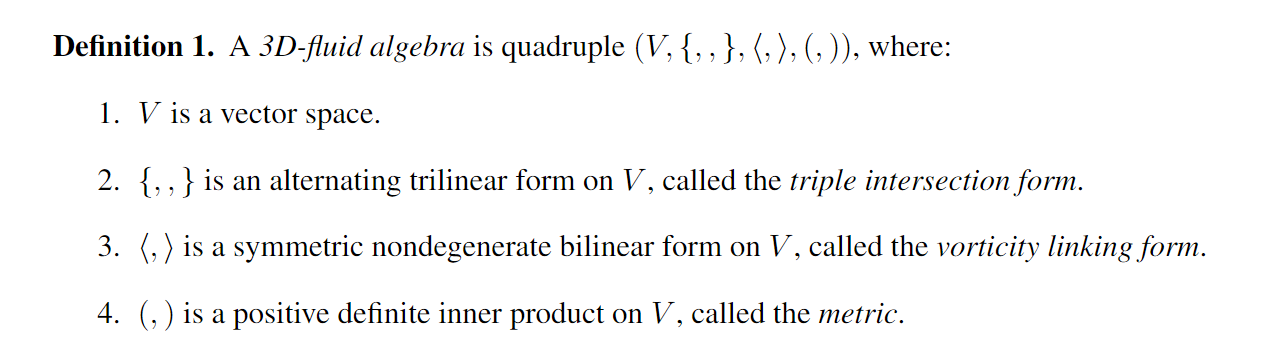
\includegraphics{figures/fluid_algebra.png}
    \end{figure}
    Maybe solenoidal beltrami fields on a compact manifold form a fluid algebra?
\end{itemize}
\begin{figure}
    \centering
    \includegraphics[width=.8\textwidth]{figures/plasma_ball.png}
    \caption{I think this would be a good thing to mention with the periodic cavity example. Pretty obvious relative homology classes.}
\end{figure}
\begin{itemize}
    \item Colin: It is probably worth reading Gross--Kotiuga \cite{gross_electromagnetic_2004}, specifically starting at page 99 and seeing what more we can do then they do. They mention Greenberg--Harper \url{http://aix1.uottawa.ca/~rblute/COURSE2/Greenberg-Harper.pdf} for Alexander duality. Gross--Kotiuga really don't think about 4 dimensional topology at all though. I think that is where we have room to do quite a bit more. All the duality theorems are still readily usable. We should be able to extract anything they do from the 4d theory. Likewise, their work doesn't really seem to \emph{do} anything as far as circuits/measurement go with the topology. So that's actually still useful. They do get into FEM methods which could maybe be useful some day for plasma related problems.
    \item Colin: I think we should reach out to Kotiuga.
    \item Colin: I've also written some stuff about Ohmic materials that may be interesting here.
    \item Colin: In 4d, are there any interesting monogenic spinor fields?
    \item The LES is physical.
    \item Kunneth theorem may also be physical.
    \item What the heck... what about excision, mayer vietoris? 
    \item Alexander duality and image charges. I think alexander duality would let you study the fields outside of conductors. For example in 3d, electric fields are relative first homology classes on the complement of a conductor. A magnetic field induces a "dual" current in the conductor. Are these somehow absolute first homology classes? Also, we tend to take the physical postulate that charges sit on the boundary of currents.
    \item What about stratified spaces? There, the homology/cohomology may not be as "symmetric"
    \item Survey of cohomological physics -- Stasheff. Reach out to him?
    \item Colin: Does taking the homotopy class of the support of a field give a map from closed fields to cycles?
\end{itemize}

\begin{itemize}
    \item Who is the intended audience? How much detail? 
    \item Measurement devices and how they work in certain ways. Volt meter (0 current?), current meter (1 current?), ohm meter is some kind of combination of both (a pairing?)
    \item "on the mathematical foundations of electrical circuit theory"  \url{https://projecteuclid.org/journals/journal-of-differential-geometry/volume-7/issue-1-2/On-the-mathematical-foundations-of-electrical-circuit-theory/10.4310/jdg/1214430827.full}
    \item permeability and permitivity play the same role as resistance in the duality?
    \item Different coefficient rings?
    \item only access to $\partial M$. What can this tell you in the LES?
    \item \url{https://ncatlab.org/johnbaez/show/Circuit+theory}
    \item interesting 4-manifolds? Interesting 3 manifold $\times S^1$. List of ones that physicists use. Ideally with some boundary. Black hole/worm hole schwarzchild metric.
    \item \url{https://www.sciencedirect.com/science/article/abs/pii/0003491657900490}
    \item Foliations. Reeb foliation (can't be level surfaces to a charge distribution but it could for a magnetic potential?? I am lost on this one) and potential fields?
    \item Hodge star is the only place where geometry shows up.
\end{itemize}

\tableofcontents

\section{Introduction}
Electromagnetism is fundamentally topological \cite{gross_electromagnetic_2004}. 
This has been understood nearly since inception. 
Maxwell, for example, was aware of the topological nature of the electromagnetic fields and referred to a measure of ``cyclosis" which is akin to the Betti numbers of a manifold. 
He knew that the topology of the domain was intimately related to the existence of certain types of functions.
 For example, \cite[theorem 1]{maxwell_treatise_1873} implies that the vanishing of the first homology class $H_1(M)$ of the body $M$ implies the existence of potentials. 
 It was not long after that de Rham \colin{cite}, Poincar\'e, and Lefschetz related the homology of a manifold to the cohomology of the forms supported on the manifold.

It would be wonderful to make this theory more approachable and intuitive. 
This means collecting all the disparate information in one place and providing the practicioner with real computational tools. 
For example, we can provide new ways for more theoretical computations like the cap product and extend this to Poincar\'e--Lefschetz duality. 
Similarly, from a unified perspective we, much of the pedogogy can be simplified. 
Certain intuitions engineers may have about electrical components can be extracted purely using topology.


When working with the homology and cohomology of manifolds there one can choose to work with the notions of simplicial, singular, and de Rham theories. 
They all end up equivalent so long as the underlying ring is a field. 
Each just with their own interpretation. 
Working with simplicial theories leads you to a realm of discrete exterior calculus \colin{cite marsden and also krane}. 
This is immensely powerful since all the features are easily computed. 
We will not focus on the simplicial theory in this paper, but will mention that \cite{hatcher_algebraic_2002} proves their equivalence. 
Singular theories lay the foundation of the theoretical tools and are the bridge for equivalence between the three choices. 
Finally, the de Rham theories are deeply analytical. 
This concerns the existence and uniqueness of fields that satisfy partial differential equations and boundary constraints.

The singular theory builds up the topological theory of spaces by continuous maps of chains. 
We can think of the image of these chains $C$ as submanifolds of a larger manifold $M$. 
Each chain is parameterized by their tangent or, equivalently, normal spaces inside of the tangent space to $M$. 
Given a chain $C_k$ of dimension $k$, we can measure the amount of a $k$-vector field $A^k$ lies tangent to $C_k$. 
This pairing amounts to integration. 

The de Rham theory uses exterior calculus and is the link to partial differential equations. 
Most commonly studied is the de Rham cohomology of differential forms, but there is also the lesser known de Rham homology of currents. 
Differential forms are a typical way to generalize the vector calculus of Heaviside and Helmholtz \colin{cite} to manifolds of arbitrary dimension. 
The measurements of differential forms are what de Rham referred to as currents. 

The most important theorem with differential forms is Stokes' theorem. 
It explains the the duality between taking the derivative of a form and the boundary of a chain. 
It is seen in many guises including the fundamental theorem of calculus, the divergence theorem, and Stokes' theorem for curves and surfaces, but it is a far more general fact. 
It also gives rise to the ever important integration-by-parts formula which we refer to a Green's formula. 
Stokes' theorem is the essential link to boundary value problems.

When studying boundary value problems, another tool is Hodge theory. 
This arises for Riemannian manifolds, that is, manifolds with a distance metric. 
This is the most analytical regime we consider. 
Here, spaces of forms are decomposed by their analytical properties. 
Remarkably, these properties align with the topological properties of the space the forms are defined on. 
That association is only possible due to both Hodge and de Rham. 
More or less, the pairing by integration mentioned previously is shown to be nondegenerate. 
This provides us an definite inner product of forms that allows for a weakening of the partial differential equations. 
This relies firmly on the manifold having a true distance measure.

Not all manifolds are lucky enough to be provided with a distance metric, but have something close. 
The predominant example are spacetime manifolds. 
In this case, there are leaves of the manifold with a spatial structure, but the manifold as a whole does not carry such a metric. 
Hence, we lose Hodge theory on the entirety of the manifold, but retain it on the leaves. 
Fortunately, there are tools to use to mitigate this issue as best as possible.

It was Grassmann who first extended vector spaces to their exterior algebra\colin{cite}. 
Not long after, Clifford added a new relation to Grassman's exterior algebra in the form of an interior multiplication. 
This small change allows for a much richer geometric algebra. 
For us, it is fortunate since it encapsulates exterior differential forms and more. 
For example, both the complex and quaternion algebras are sub-Clifford algebras in an intuitive way. 
They are actually sums of multiple graded elements.

% talk about relative stuff and why poincare duality should be true via flux and work


\subsection{Integration and Relation to Forms}

Integration on manifolds requires differential forms. In essence, a differential form consists of a $k$-vector fields with an attached coordinate measure. Let the measures be $dx^i$ in local coordinates and let $\blade{e}^i$ be the corresponding reciprocal vectors. The \emph{basic directed measures} are $d\blade{x}^i = \blade{e}^i dx^i$ (no summation implied) and they determine the \emph{$k$-dimensional directed measures}
\begin{equation}
    dX_k \coloneqq \frac{1}{k!} \sum_{i_1 < \cdots < i_k} d\blade{x}^{i_1}\wedge \cdots \wedge d\blade{x}^{i_k} = \frac{1}{k!} \sum_{\mathcal{I}} \blade{E}_{\mathcal{I}} dx^{\mathcal{I}}
\end{equation}
An arbitrary differential $k$-form $\alpha_k$ is given by taking a corresponding $k$-vector $A_k$ and contracting along the $k$-dimensional directed measure
\begin{equation}
\alpha_k = A_k \contract dX_k^\dagger.
\end{equation}
Specifically, $A_k = \sum_{\mathcal{I}} \alpha_{\mathcal{I}} \blade{E}^{\mathcal{I}}$ is called the \emph{multivector equivalent of $\alpha_k$}. This is a realization of the isomorphism between $\G(M)$ and $\Omega(M)$ as $C^\infty(M)$-modules and it can be viewed as an extension of the musical isomorphisms \cite[chapter 13]{lee_introduction_2012}. 

Since our manifold carries a nonsingular $g$, we have a volume form $\mu$ which has the multivector equivalent $\pseudoscalar^{-1 \dagger}$ which we can see by referencing \cref{eq:volume_scaling} and in this case we get the volume scale factor $\sqrt{|\det g|}$. We can note as well $\blade{I}(x)$ represents the tangent space $T_x M$. When $\partial M \neq \emptyset$, we have the \emph{boundary pseuodoscalar} $\blade{I}_\partial$ and dual to this the boundary normal field $\normal = \pseudoscalar_\partial^\perp$. As on $M$, $\blade{I}_\partial^{-1 \dagger}$ is the multivector equivalent of the boundary area form $\mu_\partial$. From this point forward, we work solely with multivector fields and contract with directed measures to integrate. 

For smooth $k$-forms $\alpha_k$ and $\beta_k$, we have an $L^2$-inner product 
\begin{equation}
\int_M \alpha_k \wedge \star \beta_k 
\end{equation}
where $\star$ is the Hodge star. By definition, the Hodge star acts on $k$-forms by returning a Hodge dual $n-k$-form so that on the multivector equivalents we have
\begin{equation}
\alpha_k \wedge \star \beta_k  = (A_k,B_k)\mu
\end{equation}
as well as
\begin{equation}
    \alpha_k \wedge \star \alpha_k = |A_k|^2\mu.
\end{equation}
For the action of $\star$ on the multivector equivalents we will put $B_k^\star$ for which we have
\begin{equation}
B_k^\star = (\pseudoscalar^{-1} B_k)^\dagger
\end{equation}
and we can quickly verify that
\begin{align}
\alpha_k \wedge \star \beta_k = (A_k \wedge B_k^\star)\contract dX_n^\dagger  =(A_k\contract B_k^\dagger) \pseudoscalar^{-1 \dagger} \contract dX_n^\dagger = (A_k,B_k)\mu.
\end{align}
If we compute $d$ and $\delta$ on forms, then we see that on the multivector equivalents
\begin{align}
\label{eq:hodge_star}
d \alpha_k &= (\grad \wedge A_k) \contract dX_{k+1}^\dagger, & \delta \alpha_k &= (-\grad \contract A_k)\contract dX_{k-1}^\dagger,
\end{align}
since, by definition, $\delta = (-1)^{n(k+1)+1+p}\star d \star$. 

The Hodge star allows us to define can now define an $L^2$ inner product forms and we can do so on multivector fields as well.
\begin{definition}
\label{def:multivector_field_inner_product}
Let $A$ and $B$ be multivector fields. Then the \emph{multivector field inner product} is defined by
\begin{equation}
\label{eq:multivecinnerproduct}
\multivecinnerproduct{A}{B} \coloneqq \int_M (A,B) \mu.
\end{equation}
If $\multivecinnerproduct{A}{B} = 0$, then we say the fields $A$ and $B$ are \emph{orthogonal}.
\end{definition}
It is clear from \cref{eq:hodge_star} that \cref{eq:multivecinnerproduct} on multivector equivalents is equal to the $L^2$ product on forms. We note that the multivector field inner product is only definite when $g$ is definite. The orthogonal direct sum with respect to the $L^2$ multivector inner product agrees with the grade based direct sum. It will suffice to use the symbol $\oplus$ for both. One should view this as a slight extension to the $r$-form inner product that garners the ability to consider the inner product of elements that are not necessarily homogeneous in grade. 

\begin{remark}
It may seem like it takes a bit of finesse to retrieve what the Hodge star does for forms, but we can see a bit more of the details of what the star does in this format. It's also worth noting that the inner product of multivector fields is notationally a bit more convenient and relates to the inner product on $\G$ more naturally.
\end{remark}

\subsection{Stokes' and Green's Formula}

\colin{I think it would be much easier to redo this little section in terms of chains and integrating $k$-vectors on $k$-chains}

\subsubsection{Arbitrary Submanifolds}
Let $K$ be a $k$-dimensional submanifold of $K$, $\pseudoscalar_K$ be the unit pseudoscalar field on $K$, and let $\mu_K$ be the volume measure. Given $K$ is a submanifold of $M$, for any $x \in K$ we have tangent space $T_x K$ which is a subspace of $T_x K$. There is also the normal space $N_x K$ that is everywhere orthogonal to $T_x K$ with respect to $g$ on $M$. This is a orthogonal subspace decomposition $T_x M = T_x K \oplus N_x K$. As in \cref{eq:dual_motivation}, we get $\normal_K = \pseudoscalar_K^\perp$ that represents the subspace $N_x K$ and $\pseudoscalar_k \wedge \normal_K = \pseudoscalar$.

We can put $\blade{I}_K(x)^{-1 \dagger}$ to be the multivector equivalent of $\mu_K$ by
\begin{equation}
\label{eq:submanifold_volume_form}
\mu_K = \blade{I}_K^{-1 \dagger} \cdot dX_r^\dagger = \blade{I}_K^{-1} \cdot dX_k.
\end{equation}
Please do note that implicit in this definition is the support of $\pseudoscalar_K$ is $K$. If one would like, you can attach the indicator function $\chi_K$ to the fields and measures, but in our notation we assume $\chi_K \pseudoscalar_K = \pseudoscalar$ as well as $\chi_k \mu_K = \mu_K$. 

\colin{I am concerned about this a bit. But the restriction I was defining seems to coincide with \url{https://physics.stackexchange.com/questions/446404/what-is-the-length-of-null-geodesic}}
\begin{remark}
Note that if $K$ is a null submanifold, then $K$ has no intrinsic volume. Take for instance a light-like curve.
\end{remark}

\begin{definition}
An $\ell$-vector field $A_\ell$ is \empph{tangent to a submanifold $K$} if
\begin{equation}
    \projection_{\pseudoscalar_K}(A_\ell)=A_\ell.
\end{equation}
\end{definition}
The notion of being tangent coincides with the pullback of inclusion of the submanifold $K\hookrightarrow M$ in the following sense.
\begin{proposition}
Let $\alpha_\ell$ be an $\ell$-form with multivector equivalent $A_\ell$ defined on $M$ and let $\iota \colon K \to M$ be the inclusion of the submanifold $K$ into $M$. Then the pullback $\iota^*$ on $\alpha_\ell$ corresponds to 
\begin{equation}
\iota^* \alpha_\ell = \projection_{\pseudoscalar_K}(A_\ell) \cdot dX_\ell^\dagger
\end{equation}
on the multivector equivalent. Furthermore, if $\ell=k$, then
\begin{equation}
\label{eq:pullback_of_k_form}
    \iota^* \alpha_k = (A_k, \pseudoscalar_K) \mu_K.
\end{equation}
\end{proposition}
\begin{proof}
Let $\blade{v}_1,\dots,\blade{v}_\ell \in T_x M$ and note that by definition of the pullback we have
\begin{equation}
    (\iota^* \alpha_\ell)_x (\blade{v}_1,\dots,\blade{v}_\ell) = (\alpha_s)_x(d\iota_x\blade{v}_1,\dots, d\iota_x\blade{v}_\ell ),
\end{equation}
Then, since $\iota$ is inclusion, we have $d\iota_x = \projection_{\pseudoscalar_K(x)}$ at each point $x \in K$ and hence $\iota^* \alpha_\ell = \alpha_\ell \circ \projection_{\pseudoscalar_K}$. For all $\blade{v}_i$ we can put
\begin{equation}
    \blade{v}_i = \projection_{\pseudoscalar_K}(\blade{v}_i) + \projection_{\normal_K}(\blade{v}_i),
\end{equation}
and note for the multivector equivalent
\begin{align}
(\projection_{\pseudoscalar_K}(A_\ell) \contract dX_\ell^\dagger)(\blade{v}_1,\dots,\blade{v}_\ell) &= (\projection_{\pseudoscalar_K}(A_\ell) \contract dX_\ell^\dagger)(\projection_{\pseudoscalar_K}(\blade{v}_1) + \projection_{\normal_K}(\blade{v}_1),\dots,\projection_{\pseudoscalar_K}(\blade{v}_\ell) + \projection_{\normal_K}(\blade{v}_\ell))\\
&= (\projection_{\pseudoscalar_K}(A_\ell) \contract dX_\ell^\dagger)(\projection_{\pseudoscalar_K}(\blade{v}_1),\dots,\projection_{\pseudoscalar_K}(\blade{v}_\ell))\\
&= (A_\ell \contract dX_\ell^\dagger)(\projection_{\pseudoscalar_K}(\blade{v}_1),\dots,\projection_{\pseudoscalar_K}(\blade{v}_\ell))
\end{align}
since $\projection_{\pseudoscalar_K}(A_\ell)$ is supported only on $K$. If $\ell > k$ we see that $\iota^* \alpha_\ell = 0 = \projection_{\pseudoscalar_K}(A_\ell)$. Finally, if $\ell = k$, we can note that 
\begin{equation}
    \projection_{\pseudoscalar_K}(A_k)\contract dX_k^\dagger = (A_k \contract \pseudoscalar_K)\pseudoscalar_K^{-1} \contract dX_k^\dagger =  (A_k \contract \pseudoscalar_K^\dagger)\pseudoscalar_K^{-1}^\dagger \contract dX_k^\dagger = (A_k,\pseudoscalar_K)\mu_K
\end{equation}
which finishes the proposition.
\end{proof}

\begin{remark}
If however the metric $g$ degenerates on a chain $K$, $K$ still has a well defined pseudoscalar $\pseudoscalar_K$ volume measure $\mu_K$ and we still get the action pullback of a $k$-form on the multivector equivalent by \cref{eq:pullback_of_k_form}. All that definition requires is a notion of a volume element. For example, if $\pseudoscalar_K=\blade{E}_{\mathcal{I}}$ then 
\begin{equation}
    \iota^* \alpha_k = (a_k,\pseudoscalar_K)\mu_K = a^{\mathcal{I}} \mu_K.
\end{equation}
\end{remark}


The above proposition motivates us to define the following.
\begin{definition}
Let $A\in \G(M)$ be a multivector field and $K\subset M$ a submanifold. We define the \emph{tangent part of $A$} by
\begin{equation}
    \tangentpart(A) = \projection_{\pseudoscalar_K}(A)
\end{equation}
and the \emph{normal part of $A$} by
\begin{equation}
\label{eq:normalpart_def}
    \normalpart(A) = A - \tangentpart(A).
\end{equation}
\end{definition}
These are used throughout the text \cite{schwarz_hodge_1995} and we will need them here.

\subsubsection{Boundary Submanifold}

The most natural submanifold for a manifold $M$ is the boundary $\partial M$. In this case, the boundary is codimension 1 inside $M$ and some of the computations become clearer. Let $\pseudoscalar_\boundary$ denote the tangent $n-1$-blade on $\partial M$ and build boundary measure via
\begin{equation}
\mu_\partial \coloneqq \pseudoscalar_\boundary^{-1} \cdot dX_{n-1}.
\end{equation}
The normal space is 1-dimensional and we put $\normal\coloneqq \pseudoscalar_\boundary^\perp $ to refer to the boundary normal space. 

Let us put $\G(\partial M)\coloneqq \G(M)\vert_\boundary$ to represent the space of fields defined on $\partial M$ that are restrictions of fields on $M$. This space contains field not just tangent to $\boundary$, but fields that have a normal component as well. Hence, we will need to know whether components of field is tangent or normal to the boundary $\partial M$ and this decomposition will be especially useful for studying homology and cohomology. To work this out, let $\normal,\blade{e}_1,\dots,\blade{e}_{n-1}$ be an orthornormal vector basis for $\G_xM$ for $x\in \partial M$ and let $\blade{E}_\mathcal{I}$ be the associated orthornormal basis versors. Then, for any multivector $A\in \G_xM$ we have
\begin{equation}
\label{eq:tangent_normal_decomposition}
A = \sum_{\normal \in \mathcal{I}} A^{\normal \in \mathcal{I}} \blade{E}_{\normal \in \mathcal{I}} + \sum_{{\normal \notin \mathcal{I}} } A^{{\normal \notin \mathcal{I}}} \blade{E}_{\normal \notin \mathcal{I}} 
\end{equation}
where the notation $\normal \in \mathcal{I}$ means to consider only versors who have $\normal$ appear and $\normal \notin \mathcal{I}$ takes only those where $\normal$ does not appear. It is clear that $\pseudoscalar_\boundary = \blade{e}_{1}\blade{e}_{2}\cdots \blade{e}_{n-1}$ and therefore
\begin{equation}
\label{eq:tangentpart}
\tangentpart(A) = \projection_{\pseudoscalar_\boundary}(A) = \sum_{{\normal \notin \mathcal{I}} } A^{{\normal \notin \mathcal{I}}} \blade{E}_{\normal \notin \mathcal{I}}.
\end{equation}
and hence the normal part is clear
\begin{equation}
\label{eq:normalpart}
\normalpart(A) = \sum_{\normal \in \mathcal{I}} A^{\normal \in \mathcal{I}} \blade{E}_{\normal \in \mathcal{I}}
\end{equation}
Of course, this is all done pointwise, but it extends nicely to a field $A\in \G(\partial M)$. In particular, the act of extracting the tangent and normal parts is captured by geometric multiplication. One can also think of it as a check for if characters exist in a collection of words.

\begin{proposition}
\label{prop:tangent_normal_proposition}
Let $\phi \in \G(\boundary)$, then 
\begin{enumerate}[i.]
\item $\phi \in \ker \tangentpart$ if and only if $\normal \contract \phi = 0$.
\item $\phi \in \ker \normalpart$ if and only if $\normal \wedge \phi = 0$.
\end{enumerate}
\end{proposition}
\begin{proof}
The proof is immediate given \cref{eq:tangentpart,eq:normalpart}. First, if $\phi \in \ker \tangentpart$ then $\phi = \normalpart \phi$ by \cref{eq:tangent_normal_decomposition}. Hence,
\begin{equation}
\normal \contract \phi = \sum_{{\normal \notin \mathcal{I}} } \phi^{{\normal \notin \mathcal{I}}} \normal \contract \blade{E}_{\normal \notin \mathcal{I}}
\end{equation}
but $\normal \contract \blade{E}_{\normal \notin \mathcal{I}} = 0$ and thus we have the first direction. On the other hand, if $\normal \contract \phi = 0$ then every $\phi^{\normal \in \mathcal{I}}=0$ which finishes the proof for (i). The proof for (ii) is done \emph{mutatis mutandis}.
\end{proof}

With the above work taken care of, we can now report one of the most important theorems that will underlie nearly everything we do here. We will not provide a proof for this theorem directly, but one can see \cite{schwarz_hodge_1995} for version using differential forms. We will just convert this to forms in the proof to realize this. 

\begin{theorem}[Stokes' Theorem]
Let $M$ be a manifold with boundary $\boundary$ and let $A_{n-1} \in \G(M)$ be a pseudovector field. Then,
\begin{equation}
    \label{eq:stokes_theorem}
    \int_M (\grad \wedge A_{n-1}, \pseudoscalar) \mu = \int_\boundary (A_{n-1},\pseudoscalar_\boundary)\mu_\boundary.
\end{equation}
\end{theorem}
\begin{proof}
We will work with both sides simultaneously starting with the equations for forms. Let $\alpha_{n-1}=A_{n-1}\contract dX_{n-1}$ be a $n-1$-form then we have
\begin{align}
    \int_M d\alpha_{n-1} &= \int_\boundary \iota^* \alpha_{n-1}\\
 \iff \qquad   \int_M (\grad \wedge A_{n-1})\contract dX_n^\dagger &= \int_\boundary \projection_{\pseudoscalar_\boundary}(A_{n-1})\contract dX_{n}^\dagger\\
 \iff \qquad  \int_M (\grad \wedge A_{n-1})\pseudoscalar^{\dagger} \pseudoscalar^{{-1} \dagger} dX_{n-1}^\dagger &= \int_\boundary (A_{n-1},\pseudoscalar_\boundary)\mu_\boundary\\
 \iff \qquad \int_M (\grad \wedge A_{n-1},\pseudoscalar) \mu &= \int_\boundary (A_{n-1},\pseudoscalar_\boundary)\mu_\boundary.
\end{align}
\end{proof}

The above version of Stokes' theorem decouples the geometry of the manifold and boundary in $\mu$ and $\mu_\boundary$ from the fields $\grad \wedge A_{n-1}$ and $A_{n-1}$. This, for example, becomes of use if $M$ is embedded in a higher dimensional $\R^m$ with $m>n$ or if we applied the above to a submanifold $K\subset M$. In this case
\begin{equation}
    \int_K (\grad \wedge A_{k-1},\pseudoscalar_K)\mu_K = \int_{\partial K} (A_{k-1},\pseudoscalar_{\partial K})\mu_{\partial K}.
\end{equation}
The latter fact will also be more important when we are doing homology and cohomology. Note that we could also put
\begin{equation}
    \int_K (\grad \wedge A_{k-1}, \pseudoscalar_K)\mu_K = \int_{\partial K} (\normal \wedge A_{k-1}, \pseudoscalar_K)\mu_{\partial K}.
\end{equation}
In essence, the operatation with $\grad \wedge$ on a manifold can be exchanged with operation $\normal \wedge$ on the boundary.

A dual notion of Stokes' theorem exist for vector fields. Let $\blade{v} \in \G^1(M)$ be a vector field, then $\blade{v}^\perp$ is a pseudoscalar field and $\grad \wedge \blade{v}^\perp = (\grad \contract \blade{v})^\perp$. Hence, it follows that
\begin{equation}
\label{eq:divergence_theorem}
    \int_M \grad \contract \blade{v} \mu = \int_\boundary \normal \contract \blade{v} \mu_\boundary,
\end{equation}
which is the typical form of the divergence theorem. In this sense, the operation $\grad \contract$ on the manifold is replaced by $\normal \contract$ on the boundary. It is also worth noting that more general versions of Stokes' theorem exist for multivector fields. For example, see \cite{doran_geometric_2003}. Next, we will show the Green's formula which follows directly from Stokes' theorem.

\begin{proposition}[Green's Formula]
Let $A_{k-1}, B_k \in \G(M)$, then we have Green's formula
\begin{equation}
\multivecinnerproduct{\grad \wedge A_{k-1}}{B_r} = -\multivecinnerproduct{A_{k-1}}{\grad \contract B_k} + \multivecinnerproduct{\normal \wedge A_{k-1}}{B_k}_\boundary.
\end{equation}
\end{proposition}
\begin{proof}
We have
\begin{align}
    \int_M (\grad \wedge [(A_{k-1}\contract B_k)^\perp],\pseudoscalar)\mu &= \int_M (\grad \wedge (A_{k-1} \wedge B_k^\perp),I)\mu\\
    &= \int_\boundary (A_{k-1} \wedge B_k^\perp, \pseudoscalar_\boundary) \mu_\boundary\\
    &= \int_\boundary ((A_{k-1} \contract B_k) \pseudoscalar^{-1} \pseudoscalar^\dagger,\normal) \mu_\boundary &&\textrm{since $\normal = \pseudoscalar_\boundary^\perp$ and $\dagger$ is the adjoint}\\
    &= (-1)^{\frac{n(n-1)}{2}} \int_\boundary (A_{k-1} \contract B_r, \normal)\mu\\
    &= (-1)^{\frac{n(n-1)}{2}} \int_\boundary (\normal \wedge A_{k-1}, B_r)\mu
\end{align}
since $\pseudoscalar^\dagger = (-1)^{\frac{n(n-1)}{2}} \pseudoscalar$. On the other hand,
\begin{align}
    \int_M (\grad \wedge (A_{k-1} \wedge B_k^\perp),\pseudoscalar)\mu &= \int_M \left( (\grad \wedge A_{k-1})\wedge B_r^\perp + (-1)^{k-1} A_{k-1} \wedge (\grad \wedge B_k^\perp),\pseudoscalar \right) \mu\\
    &= \int_M \left( [(\grad \wedge A_{k-1}) \contract B_{k}]^\perp , \pseudoscalar \right)\mu + (-1)^{k-1} \int_M \left( [A_{k-1} \contract (\grad \contract B_k)]^\perp, \pseudoscalar \right)\mu \\
    &=(-1)^{\frac{n(n-1)}{2}} \int_M \proj{}{(\grad \wedge A_{k-1})  B_{k}}\mu + (-1)^{k-1 + \frac{n(n-1)}{2}} \int_M \proj{}{ A_{k-1} (\grad \contract B_k)}\mu\\
    &=(-1)^{\frac{n(n-1)}{2} + \frac{k(k-1)}{2}} \multivecinnerproduct{\grad \wedge A_{k-1}}{B_k} + (-1)^{\frac{n(n-1)}{2} + \frac{k(k-1)}{2}} \multivecinnerproduct{A_{k-1}}{\grad \contract B_r}.
\end{align}
Hence, we have our proof by moving the $\dagger$ to $B_k$.
\end{proof}

Finally, it is worth noting that from the Green's formula, we get the special case:
\begin{equation}
    \label{eq:special_greens_formula}
\multivecinnerproduct{\grad \wedge A_{k}}{\grad \wedge A_{k}}_M + \multivecinnerproduct{\grad \contract A_{k}}{\grad \contract A_{k}}_M = \multivecinnerproduct{-\grad^2 A_k }{A_k}_M  +  \multivecinnerproduct{\normal \wedge A_k}{\grad \wedge A_k}_\boundary + \multivecinnerproduct{\grad \contract A_k}{\normal \contract A_k}_\boundary.
\end{equation}
The fact that $-\grad^2$ is positive definite when $g$ is positive definite is of utmost importance in Hodge theory. 
\colin{I think this equation basically captures everything about cohomology at once.}

%---------------------------------------------------------------------------------------------------------------------------

%---------------------------------------------------------------------------------------------------------------------------
\subsection{Currents}
\label{sec:fields_and_currents}
%---------------------------------------------------------------------------------------------------------------------------

Currents were introduced by de Rham in \colin{add a citation to the OG de Rham paper} as dual objects to (i.e., functionals on) the space of differential forms. Physically, we should think of currents as a means of measuring fields. Take for instance a smooth field $f\in \G(M)$; there are many questions we can ask about this field, e.g., at any $x\in M$ we can ask for any order derivative of $f$ or point value for $f$. For example, asking for the point value corresponds to the Dirac mass current $\delta_x$ defined by evaluation $\delta_x(f)=f(x)$. We could find the flux of $f$ through some object or the flow of $f$ along another object and in some circumstances these answers are the same. 

Of course, we can string together multiple such measurements together to produce a more involved measurement. The space of measurements far larger than just the space of fields we are measuring. We can see that the currents contain the fields themselves since we imagine we know some field $g$ and use it a means to measure the field $f$. However, the current $\delta_x$ is not a smooth field and this is a valid measurement.

Let us examine the classical examples of flux and circulation. Let $\blade{v}\in \G^1(M)$ be a vector field and $\gamma$ a 1-dimensional piecewise continuous curve, i.e., we have the tangent pseudoscalar $\pseudoscalar_C$ which is a piecwise continuous vector field supported on $\gamma$. The \emph{current of circulation} is
\begin{equation}
\label{eq:circulation_current}
    \mathrm{Circulation}_C(\blade{v}) = \int_C (\blade{E}, \pseudoscalar_\gamma) \mu_\gamma.
\end{equation}
The possible corners in $\gamma$ do not factor into the integral since they are a set of measure zero. The current of circulation is maximized when $\blade{v}$ is tangent to $\gamma$ and maintains the same orientation over $\gamma$. That is exactly what this current seeks to measure, after all. For a physicist, this current could be a means to measure work done on a particle that traverses the path $\gamma$ and $\blade{v}$ would represent a force vector field.

If we move up a dimension, we can take $\blade{b}\in \G^2(M)$ and a piecewise continuous surface $S$ with tangent pseudoscalar $\pseudoscalar_S$. The \emph{current of flux} is
\begin{equation}
\label{eq:flux_motivation}
    \mathrm{Flux}_S(\blade{b}) = \int_S (\blade{b},\pseudoscalar_S) \mu_S
\end{equation}
This current is again maximal when $\blade{b}$ lies tangent and oriented with $S$. 

A discussion is in order. A physicist likely thinks of flux as the amount of a field that passes through a surface. So what is the deal here? The deal is that our eyes view this problem in 3-dimensions and that we are taught to picture vector fields and not bivector fields. Also, this has never been a problem in 3-dimensions, so why bring it up?

It turns out that every bivector in 3-dimensions is a 2-blade. Hence, every bivector $\blade{b}$ both determines a unique vector $\blade{b}^\perp$ and vice versa. We have never had to work to visualize bivectors because there is no scenario that requires it in 3-dimensions. This is not true in 4-dimensions! At any rate, we can see what a bivector field looks like in 3-dimensions. We visualize it as a plane field like \cref{fig:plane_field} and see its dual field by \cref{fig:vector_field}. 
\begin{figure}[H]
\centering
\begin{subfigure}[b]{0.49\textwidth}
    \centering
    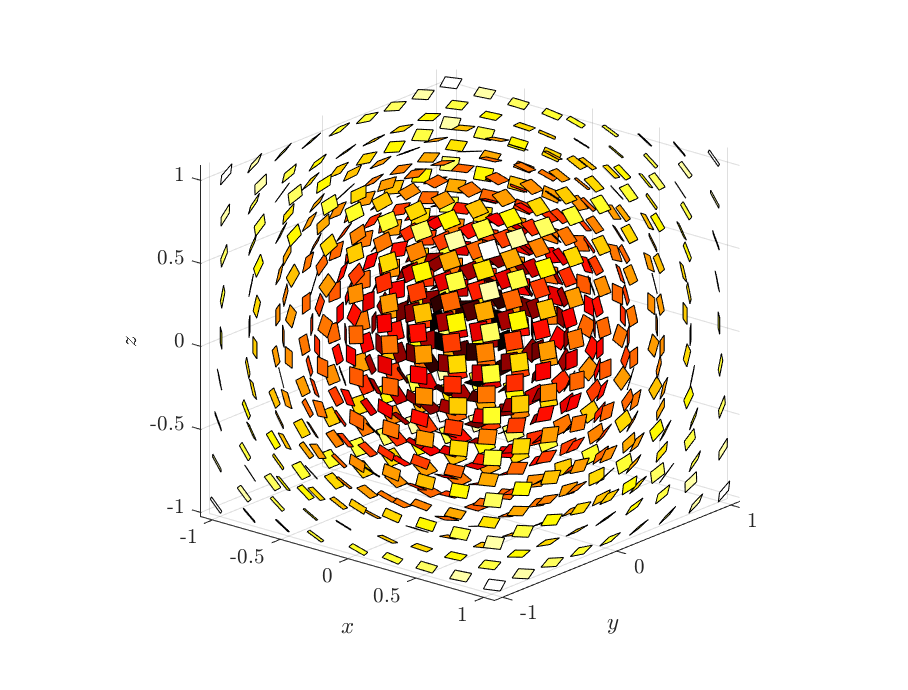
\includegraphics[width=\textwidth]{figures/plane_field}
    \caption{A bivector field corresponding to $\blade{b}=x \blade{E}_{23} + y\blade{E}_{31} + z\blade{E}_{12}$}
    \label{fig:plane_field}
\end{subfigure}
\begin{subfigure}[b]{0.49\textwidth}
    \centering
    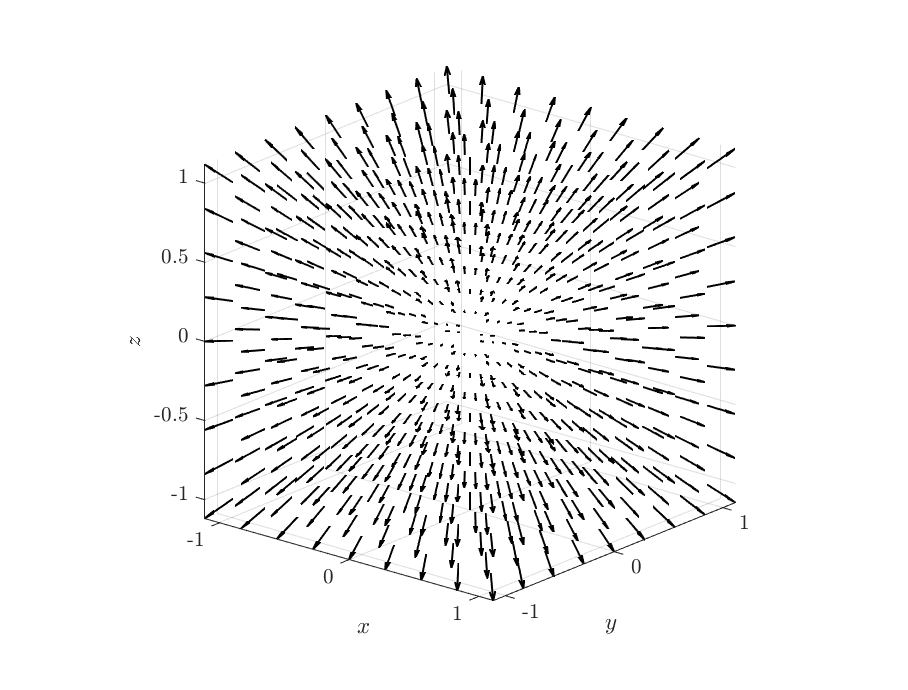
\includegraphics[width=\textwidth]{figures/vector_field}
    \caption{The dual vector field corresponding to $\blade{b}^\perp =x \blade{e}_{1} + y\blade{e}_{2} + z\blade{e}_{3}$}
    \label{fig:vector_field}
\end{subfigure}
\end{figure}
The color of the planes represents the magnitude of the bivector. If we look at all the planes with the same color, we see that these constitute the area elements of a 2-sphere of a constant radius! This goes to show that while a 2-sphere may not have a nowhere vanishing tangent vector field (Hairy ball theorem), it does have a nowhere vanishing bivector field. This is not exactly surprising since this is really the area element and it is also dual (intrinsically) to the scalar fields on the sphere.

What can we glean from Stokes' theorem? First, if $C$ bounds some surface $S$, then we say $C=\partial S$. Then it must be that
\begin{equation}
    \mathrm{Circulation}_{C}(\blade{v}) = \mathrm{Flux}_{S}(\grad \wedge \blade{v}).
\end{equation}
But, if $C$ bounds no surface $S$, the above cannot be true! This fact will come back as the notion of a \emph{period} and it is essential in understanding the role of (co)homology will play for us. We could also have supposed that $\blade{b}=\grad \wedge \blade{v}$ from the outright in which we must have
\begin{equation}
    \mathrm{Flux}_S (\blade{b})=\mathrm{Circulation}_{\partial S}(\blade{v}).
\end{equation}
As you can see, moving from $\grad \wedge$ on a field necessitates we can apply $\partial$ to the region in which we integrate. However, the other way is not true. Not all curves bound a surface.  

A similar argument of course can be done for the divergence theorem. In that case $\grad \wedge \blade{b}$ is a measure of divergence. One will come to the realization that not all surfaces in $\R^3$ bound a volume and so not all divergence free bivector fields are curls of vector fields.

As a last point, in 4-dimensions, e.g., Minkowski space, there are bivectors that are not 2-blades. For instance the the most general bivector
\begin{equation}
    F =  E^1 \blade{e}_0 \blade{e}_1 + E^2 \blade{e}_0 \blade{e}_2 + E^3 \blade{e}_0 \blade{e}_3 + B^{3} \blade{e}_1 \blade{e}_2 + B^{2} \blade{e}_3 \blade{e}_1 + B^{1} \blade{e}_2 \blade{e}_3.
\end{equation}
cannot in general be written as the exterior product of two vectors. This has immense physical ramifications that we discuss later. \textcolor{red}{A reasonable question would be if a bivector field $\blade{b}$ can be written as a product of two vector fields (even locally) $\blade{v}\wedge \blade{w} = \blade{b}$. Is it true that if $\grad \blade{b}=0$ then this is true? This seems like an integrability condition. It could also be with the helicity $\blade{b} \wedge (\grad \wedge \blade{b})=0$ (or actually $\blade{b} \wedge (\grad \contract \blade{b})$. Non-example would be the standard contact structure. Globally, there would also be issues with spheres, but if we just care about locally then this is fine. It's probably just worth writing this out}


\subsubsection{Definitions and Examples}
Since we have captured differential forms in terms of multivectors, we can also capture \emph{de Rham currents} $\Omega(M)^*$ as functionals on $\G(M)$. Specifically, this is because $\G(M)\cong \Omega(M)$ as $C^\infty$-modules by \cref{eq:musical_iso_generalization}. The space of linear maps $\G(M) \to \R$ which we write as $\G(M)^*$ is thus isomorphic to $\Omega(M)^*$ as modules.
\begin{definition}
A \emph{current} is a linear functional $\G(M) \to \R$ and we put $\G^*(M)$ to represent the space of currents. An \emph{$k$-current} is a linear functional $\G^k(M) \to \R$ and we put $\G^{k}(M)^*$ to represent the space of $k$-currents.
\end{definition}
By linearity, it follows that
\begin{equation}
\G^*(M) = \bigoplus_{k = 1}^n \G^{k*}(M).
\end{equation}
\colin{Should probably preface this with the fact that we just want normal currents.\url{https://www.jstor.org/stable/pdf/1970227.pdf}}

Given a $k$-current $B^k \in \G^k(M)^*$ we denote the pairing with a $k$-vector $A_k \in \G^k(M)$ by $B^k(A_k)$. We will use superscripts for currents to distinguish the duality. There are two canonical ways we could define a $k$-current. We will show that, at least up to homology, they are interchangeable.

\begin{enumerate}[i.]
    \item Given a $k$-vector $B_{k}$ we can define the \emph{current of the $k$-vector field} $B^k\in \G^k(M)^*$ by
\begin{equation}
\label{eq:multivector_current}
    B^k(A_k) \coloneqq \int_M (A_k,B_k) \mu.
\end{equation}

    \item We can take an continuous $k$-chain $\chain{C}^k$ and note that the \emph{current of the $k$-chain} $C^k \in \G^k(M)^*$ is given by
\begin{equation}
\label{eq:chain_current}
    C^k(A_k) \coloneqq \int_{\mathscr{C}^k} (A_k, \pseudoscalar_{\chain{C}^k}) \mu_{\chain{C}^k}
\end{equation}
\end{enumerate}
Given that $\chain{C}^k$ is continuous, its tangent pseudoscalar $\pseudoscalar_{\chain{C}^k}$ can be thought of as a limit of smooth $k$-blades defined in a neighborhood of $\chain{C}^k$. In this sense, the current of the $k$-chain $C^k$ is really just a current of a $k$-vector $\pseudoscalar_{\chain{C}^k}\in \overline{\G^k(M)}$. 

We mentioned another example of a current of a chain before: take a point $x$, then the 0-current $\delta_x$ is the Dirac mass
\begin{equation}
\delta_x[A_0] = A_0(x).
\end{equation}
But of course, we may want to measure other parts of a general multivector $A$. For instance, we have the current $\delta_{\blade{E}_\mathcal{I},x}$
\begin{equation}
    \delta_{\blade{E}_\mathcal{I},x}(A) = (A(x),\blade{E}_\mathcal{I}) = A^\mathcal{I}(x).
\end{equation}
It is possible to define currents that take value in $\G$. This study is fruitful. For example, see \colin{cite my paper}.

\begin{example}[Helicity]
As a final example, let us consider helicity. Helicity is a measure of the twist of a vector field relative to a corresponding bivector field. In particular, Let $\blade{v}$ be a vector field and $\chain{C}^3$ be a 3-chain, then the \emph{helicity current on $\chain{C}^3$} is
\begin{equation}
    \mathrm{Helicity}_{\chain{C}^3}(\blade{v}) = \int_{\chain{C}^3}(\blade{v} \wedge (\grad \wedge \blade{v}), \pseudoscalar_{\chain{C}^3})\mu_{\chain{C}^3}.
\end{equation}
This is a wonderful measurement of magnetic fields that measures the intersection of flow lines of the field $\blade{v}$ with the plane $\grad \wedge\blade{v}$ on a 3-dimensional body. Equivalently, it is a linking between integral curves of $\blade{v}$ and integral curves of $(\grad \wedge \blade{v})^\perp$. We can retrieve this as a topological property later.\colin{It would be amazing to show this is computing linking using intersection/alexander duality. The $\perp$ duality should make for nice pictures too. Now, are there more general currents that could correspond to Massey products that may be really really interesting.}
\end{example}

The point of introducing currents is to bring in the idea of measurements of fields in geometry and topology. It turns out that the space of currents is rather unwieldy. So we will find ourselves reducing to currents built from continuous chains and fields. For a far more in depth journey into currents, please see \cite{giaquinta_cartesian_1998}.


%---------------------------------------------------------------------------------------------------------------------------
\section{Homology and Cohomology}\label{sec:homology_and_cohomology}
%---------------------------------------------------------------------------------------------------------------------------

One reason to care about manifolds $M$ as a whole is to consider physics constrained to geometries beyond $\R^n$. Much of physics cares about the local geometric structure, for example, the flow of electrical current at a point in $M$ depends on the conductivity neighboring that point. Electric current follows the path of least resistance and geometrically this is akin to following local geodesics. In fact, the conductivity matrix is related to a Riemannian metric very explicitly. This idea gave rise to the Calder\'on problem for manifolds and more can be found in \colin{cite uhlmann}.

At a more coarse scale, we know current flows from regions of higher voltage to lower voltage or is induced by a magnetic field, both can be attributed to the Lorentz force. We do not need access to metric information to get the big picture. As it turns out, the topology of the domain is intimately related to the existence of physical phenomena of fields. Hence, topological laws of nature are very qualitative and extremely robust to deformation. This is not only useful for intuitive computation, but it is ripe for pedagogy. Homology and cohomology will prove to be what we want to work with at first.

Think of a physics problem cast as a Partial Differential Equation (PDE). In $\R^3$ one can ask if the PDE for a potential $\grad \wedge \phi = \blade{v}$ is uniquely solvable for the scalar field $\phi$ for any any given vector field $\blade{v}$. A classical fact is that if $\blade{v}$ is curl-free, $\grad \wedge \blade{v}=0$, then $\phi$ exists but is not unique, as $\phi$ is determined up to a constant. The constant $c$, of course, satisfies $\grad \wedge c=0$, hence we can only find an equivalence class of $\phi$ uniquely. Of course, we know $(\grad \wedge)^2  =0$ is inherent to $\grad \wedge$ for any field, but if we change the topology of the underlying space this turns out to not be so easy.

If our space $M$ is not simply connected, then there is a loop in $M$ that cannot be contracted to a point. In that case, we can build a vector field $\blade{v}$ tangent to the loop with $\grad \wedge \blade{v}=0$, but there is no way that $\blade{v}=\grad \wedge \phi$ for any scalar $\phi$. There is no real Escher's staircase after all \colin{cite keenan crane and probably use his picture}! \colin{Okay but you could build a field on the universal cover of the loop and map this down. Since the curve is an image of a Lie group $S^1$, this map from the cover $\R$ to $S^1$ is a homomorphism. Does this do anything for us? Also, this could be sheafy. There would be a multivalued potential. Kotiuga uses this in his book/thesis}

\colin{Terry Tao: de Rham cohomology is a measure of the failure of the fundamental theorem of calculus}

\subsection{Homology}
\label{subsec:homology}

\subsubsection{Homology Theory}
 \colin{I can probably shorten this by quite a bit. I'm just not sure what level of expertise we want to assume here.}
Homology measures the connected components, holes, cavities, and generalizations thereof inside of spaces. Our spaces are manifolds $M$ and are sufficiently nice to think about. Homology is also defined in a handful of ways! 
\begin{enumerate}
    \item \emph{Simplicial homology} $H_{k,\Delta}(X)$ is a way to compute homology on simplicial complexes $X$ which are built from simplices. Simplices are, intuitively speaking, a triangular mesh of an $n$-dimensional object. A simplicial chain $C_{k,\Delta}$ is a complex built only out of $k$-dimensional simplices.
    \item \emph{Singular homology} $H_{k,\textrm{sing}}(X)$ computes homology of $X$ by mapping simplicial $k$-chains into $X$ and we call these maps the \emph{singular $k$-chains} and put $C_{k,\textrm{sing}}(X)$. If $X=M$ is a smooth manifold, then the singular chains are the chains we have previously integrated over.
    \item \emph{de Rham homology} $H_{k,\textrm{dR}}(X)$ measures the homology of $X$ using $k$-currents.
\end{enumerate}
In each theory, we have a map $\partial$ called the \emph{boundary map} that acts on chains $C_k(X)$ by $\partial_k\colon C_k(X) \to C_{k-1}(X)$ and we use the subscript to denote which space $\partial$ is acting on. On simplicial and singular homology, $\partial$ gives you back the boundary you would expect. Chains form a free $R$-module so if $\chain{C}^k, \chain{D}^k \in C_k(X)$ and $r,q\in R$ then $r\chain{C}^k+q\chain{D}^k\in C_k(X)$ and this addition is abelian. By the universal coefficient theorem \cite{hatcher_algebraic_2002} we can always just take $R=\Z$ and tensor with other rings when necessary. For notation, we put $C_k(X;\Z)$ to distinguish the ring of the module. 

\begin{remark}
We use $X$ in place of $M$ or perhaps the pair $(M,\boundary)$ when a statement is true for either. The pair $(M,\boundary)$ appears in the relative homology and cohomology. 
\end{remark}

Moreover, we have that $\partial$ is a homomorphism and $\partial^2=0$. Hence, we have a \emph{chain complex} $(\boundary, C_\bullet(X;R))$
\begin{equation}
\cdots \to C_{k+1}(X;\Z) \xrightarrow{\partial} C_k(X;\Z) \xrightarrow{\partial} C_{k-1}(X;\Z) \to \cdots.
\end{equation}
We define the \emph{$k$-cycles} $Z_k(X;\Z)=\ker \partial_k$ and the \emph{$k$-boundaries} $B_k(X;\Z) = \im \partial_{k+1}$. Since $\partial^2=0$, $B_k(X;\Z)\subset Z_k(X;\Z)$. The purpose of homology is to measure exactly how many kinds of $k$-cycles $Z_k(X;\Z)$ are not $k$-boundaries $B_k$. 
\begin{definition}
The $k$th homology of $X$ is the free $\Z$-module
\begin{equation}
    H_k(X;R) \coloneqq Z_k(X;\Z)/B_k(X;\Z).
\end{equation}
\end{definition}
Hence elements of $H_k(X;\Z)$ are equivalence classes $[A]$ and $[B]$ of cycles $A$ and $B$ whose difference between them is a boundary: 
\begin{equation}
[A]=[B] ~ \iff ~ A=B+\partial C.
\end{equation}

For topological spaces, the notion of a boundary is well defined and this is what we take as $\partial$. Furthermore, it is a fact that the singular and simplicial homology theories are equivalent (see \cite{hatcher_algebraic_2002}). It would be nice to realize the same is true for the de Rham homology.

\colin{Compact with boundary or mention that currents are compactly supported}
On currents we build the de Rham homology \cite{iversen_cauchy_1989,lekhyananda_homology_nodate, giaquinta_cartesian_1998} by defining the boundary operator $\partial$ on $k$-currents $B^k \in \G^{k*}(M)$ by passing to the smooth fields in the following way. Let $A_{k-1}\in \G^{k-1}(M)$ be a $(k-1)$-vector field, then
\begin{equation}
\partial B^{k}[A_{k-1}] \coloneqq B^{k}[\grad \wedge A_{k-1}].
\end{equation}
Since we can always depend on the smoothness of fields that currents are applied to, the boundary map is well defined and it is also clear that $\partial^2 = 0$ from the fact that $(\grad \wedge)^2=0$. We use the same notation for cycles and boundaries but with the added dR tag. That is, we have the \emph{de Rham $k$-cycles} $Z_{k,\mathrm{dR}}(M)$ and the \emph{de Rham $k$-boundaries} $B_{k, \mathrm{dR}}(M)$. The ring in our case is fixed to be the real field $\R$. 


\colin{I should probably use mathcal fonts or something since I Have fields $B_k$}

Let us see how this translates to the two canonical examples of currents we mentioned earlier. 

\begin{example}
\label{ex:boundaries_of_currents}
\begin{enumerate}[i.]
    \item Let $B^{k}\in \G^k(M)^*$ be a current of the $k$-vector field $B_{k}$, then 
\begin{align}
    \partial B^k[A_{k-1}]&= B^k(\grad \wedge A_{k-1})\\
    &= \multivecinnerproduct{\grad \wedge A_{k-1}}{B_k}\\
    &=-\multivecinnerproduct{A_{k-1}}{\grad \contract B_k}_M + \multivecinnerproduct{A_{k-1}}{\normal \contract B_k^\dagger}_\boundary && \textrm{by Green's formula.}
\end{align}
We see that we can pass to the interior derivative on the corresponding field, but must account for boundary behavior of $B_k$ as well. In particular, if is true that $\grad \contract B_k = 0$ and $\normal \contract B_k = 0$, then $\partial B^k=0$. \colin{But this is NOT the only way this can be true if the metric has signature!}

\item Let $C^k \in \G^k(M)^*$ be the current of the $k$-chain $\chain{C}^k$ then 
    \begin{align}
        \partial C^k (B_k)&= C^k(\grad \wedge A_{k-1})\\
            &= \int_{\chain{C}^k} (\grad \wedge A_{k-1},\pseudoscalar_{\chain{C}^k})\mu_{\chain{C}^k}\\
            &= \int_{\partial \chain{C}^k} (A_{k-1},\pseudoscalar_{\partial \chain{C}^k}) \mu__{\partial \chain{C}^k} && \textrm{by Stokes' theorem.}
    \end{align}
    Hence, the boundary of the current $\partial C^k$ is the current of the $k-1$-chain $\partial \mathscr{C}^k$.
\end{enumerate}

Then the \emph{$k^\textrm{th}$ de Rham homology} is vector space of the quotient
\begin{equation}
    H_k^{dR}(M) \coloneqq Z_{k,\mathrm{dR}}(M)/B_{k, \mathrm{dR}}(M).
\end{equation}
\end{example}
\colin{These are really normal currents \url{https://www.jstor.org/stable/pdf/1970227.pdf} IS helicity a normal current? Should be if the 3 chain is compact for sure, but we may want non compact helicities?}

\begin{example}[Helicity and Beltrami Fields]\label{ex:helicity_and_beltrami}
Consider the helicity current on some 3-chain $\chain{C}^3$. Recall that this is a 1-current, so its boundary is a 0-current. Given a scalar field $\phi$ we have
\begin{align}
    \partial \mathrm{Helicity}_{\chain{C}^3}(\phi) &= \mathrm{Helicity}_{\chain{C}^3}(\grad \wedge \phi)\\
    &= \int_{\chain{C}^3}([\grad \wedge \phi] \wedge [\grad \wedge \grad \wedge \phi], \pseudoscalar_{\chain{C}^3})\mu_{\chain{C}^3}\\
    &=0 &&\textrm{since $\grad \wedge^2=0$}.
\end{align}
Hence, for any 3-chain, $\mathrm{Helicity}\in Z_{1,\mathrm{dR}}(M;\R)$ (so long as $M$ is at least 3-dimensional that is). \textcolor{red}{It is also confirming the fact that no gradient field has curl by confirming they cant have helical integral curves. It is a valid question to wonder if helicity is a boundary!}

Let us search for what $2$-current helicity would bound. We can call this PreHelicity we define it on a bivector $a_2$ by
\begin{equation}
    \mathrm{PreHelicity}_{\chain{C}^3}(a_2) \coloneqq \int_{\chain{C}^3} ([\grad \contract a_2]\wedge a_2, \pseudoscalar_{\chain{C}^3})\mu_{\chain{C}^3}.
\end{equation}
Then the boundary is defined on vector fields $\blade{v}$ and
\begin{align}
    \partial \mathrm{PreHelicity}_{\chain{C}^3}(\blade{v}) &= \mathrm{PreHelicity}(\grad \wedge \blade{v})\\
        &= \int_{\chain{C}^3} ([\grad \contract \grad \wedge \blade{v}]\wedge [\grad \wedge \blade{v}],\pseudoscalar_{\chain{C}^3})\mu_{\chain{C}^3}.
\end{align}
We see that helicity is not quite a boundary, but if $\blade{v}$ is a \emph{solenoidal Beltrami field}, then $\grad \contract \grad \wedge \blade{v} = -\lambda^2 \blade{v}$ for some $\lambda$. A Beltrami field is a field which align with their own curl or, equivalently, are perpendicular to the plane of rotation so $\blade{v} \contract (\grad \wedge \blade{v})=0$ and solenoidal implies $\grad \contract \blade{v}=0$\colin{So $\blade{v}$ is a 1st homology class and is absolute or relative depending on boundary conditions. This actually becomes a product on homologies now.}. In fact, both these facts imply $\nabla_{\blade{v}}\blade{v}=0$ and $-\grad^2 = \lambda \blade{v}$. \textcolor{red}{So Beltrami fields are autoparallel and their integral curves are locally geodesics on a cylinder and moreover the vector field is a harmonic of the vector laplacian. Of course, this is all intrinsic to $\chain{C}^3$.}
\end{example}



\subsubsection{Relative Homology}

On manifolds $M$ with boundary $\boundary$, there is another important homology to discuss. Namely, the \emph{relative homology} $H_k(M,\boundary;\Z)$. We define the \emph{relative $k$-chains} $C_k(M,\boundary;R)$ as a quotient group $C_k(M)/C_k(\boundary)$. Hence, chains in $\boundary$ are trivial in $C_k(M,\boundary)$. The boundary map $\partial \colon C_k(M)\to C_{k-1}(M)$ induces a map on the quotient $\partial \colon C_k(M;\boundary) \to C_{k-1}(M;\boundary)$ and $\partial^2=0$ still holds. The \emph{relative $k$-cycles} $Z_k(M;\boundary)$ are elements in $C_k(M;\boundary)$ that are also in the kernel of $\partial_k$ and the \emph{relative $k$-boundaries} are elements in $C_k(M;\boundary)$ that are in the image of $\partial_{k+1}$.

\begin{definition}
The \emph{relative $k$th homology group} is the quotient group
\begin{equation}
    H_k(M,\partial M;\Z) \coloneqq Z_k(M,\boundary;\Z)/B_k(M;\boundary;\Z).
\end{equation}
\end{definition}

Let us think about relative cycles and boundaries intuitively.
\begin{itemize}
    \item A relative cycle is an $k$-chain $\chain{C}^k \in C_k(M)$ such that $\partial \chain{C}^k \in C_{k-1}(\boundary)$. That is, the boundary of the relative cycle must lie in the boundary of $M$.
    \item A relative boundary is an element $\chain{C} = \partial \chain{A} + \chain{B}$ where $\chain{A} \in C_{k+1}(M)$ and $\chain{B} \in C_k(\boundary)$.
\end{itemize}

This is formalized in the \emph{long exact sequence of relative homology}. First, let us note we have maps
\[
% https://tikzcd.yichuanshen.de/#N4Igdg9gJgpgziAXAbVABwnAlgFyxMJZABgBpiBdUkANwEMAbAVxiRGJAF9T1Nd9CKAIzkqtRizYBhAPoBrABQAdJQCMITMFDoAnAJ4BKLjxAZseAkQBMo6vWatEIWYoCyR7r3MCiAZlviDtLyCq6kKuqa2voeJmb8ligALAH2kk4cnqZ8FoIkpEJiaY7sxl4JeSKFdhIlssByALRCnMpqGlq6hmXZ3onINtWB6c4yDc2t7j3xuX4FRbXBbuHtUV2x5bPJ8zVBGVxiMFAA5vBEoABmOhAAtkhkIDgQSCIgDHSqMAwACjk+TgwYBccD0rrcXtQnkgbMMSip8Dg6KDrndEDCoYh-LC2CoAFY3Og4AAWyPBiAArJDnogAGxZMGomlUpAAdl2I3hEERpNRbMe1IAHOy4Up8YSSfSUUgsRikpKyUL+UgAJzy1EywXCnFKNC6PCMHnQ5mIPnFbW6nT6hiGxCvDFM7FOFQWq0HThAA
\begin{tikzcd}
0 \arrow[r] & C_k(\boundary) \arrow[r, "\iota"] \arrow[d, "\partial"] & C_k(M) \arrow[r, "\jmath"] \arrow[d, "\partial"] & {C_k(M,\boundary)} \arrow[r] \arrow[d, "\partial"] & 0 \\
0 \arrow[r] & C_{k-1}(\boundary) \arrow[r, "\iota"]                   & C_{k-1}(M) \arrow[r, "\jmath"]                   & {C_k(M,\boundary)} \arrow[r]                       & 0
\end{tikzcd}
\]
where $\iota$ is the \emph{inclusion map} and $\jmath$ is the \emph{quotient map}. This sequence of spaces is \emph{exact} and hence $\ker \jmath = \im \iota$. From this we get the long exact sequence
\[
% https://tikzcd.yichuanshen.de/#N4Igdg9gJgpgziAXAbVABwnAlgFyxMJZARgBoAGAXVJADcBDAGwFcYkQAJAfQGsAKADoCARhGZgo9AE4BPAJQgAvqXSZc+QinIVqdJq3ZCAxlAg4Ey1djwEiAJh00GLNok5dgPRXwCyCyyAY1hpEAMyOei7s3Pw+pEKi4pKy-iqBajaayAAsEc4GbtyeALTE3gliEtLySmlB6rYoAKx5+q4gxqbmSrowUADm8ESgAGZSEAC2SGQgOBBI2pEFHQJo0nhMtaPjU4iLc0gOS+1C+Dj0XABUWyBjk4c0B4jhx4YCAFYT9DgAFlc3d12LyeuVebiEaykG0YAJ2SFBTxaYJWZwu10UlEUQA
\begin{tikzcd}
\cdots \arrow[r, "\partial"] & H_k(\boundary) \arrow[r, "\iota_*"] & H_{k}(M) \arrow[r, "\jmath_*"] & {H_k(M,\boundary)} \arrow[r, "\partial"] & H_{k-1}(\boundary) \arrow[r, "\iota_*"] & \cdots
\end{tikzcd}
\]
and by exactness $\im \iota_* \subset \ker \jmath_*$, $\im \jmath_* \subset \ker \partial$, and $\im \partial \subset \ker \iota_*$.

\begin{itemize}
    \item The inclusion map $\iota \colon C_k(\boundary) \to C_k(M)$ and its induced map $\iota_* \colon H_k(\boundary) \to H_k(M)$ on homology are clear. Given a chain on the boundary we can always include this as a chain in $M$ as an injection and pass this map to homology.
    \item The quotient map $\jmath \colon C_k(M) \to C_k(M,\boundary)$ is a bit less obvious. We take a chain on $M$ and map it to its class in the quotient group $C_k(M)/C_k(\boundary)$ as a surjection. That is, for a chain $\chain{C} \in C_k(M)$ we have the equivalence class $\jmath (\chain{C})$ up to some chain in $C_k(\boundary)$
    \item The boundary map $\partial \colon C_k(M,\boundary) \to C_{k-1}(\boundary)$ maps a relative chain to its boundary since its boundary must be in $C_{k-1}(\boundary)$ by construction. Its induced map $\partial \colon H_k(M) \to H_{k-1}(\boundary)$ extracts the homology class of the boundary of the class in $H_k(M)$.
\end{itemize}

\begin{theorem}[de Rham's Theorem for Homology]
The homologies $H_{\bullet,\textrm{sing}}(X;\R)$, and $H_{\bullet,\textrm{dR}}(X)$ are isomorphic.
\end{theorem}

The proof for the above theorem is involved, but the fact $H_{sing}\cong H_{simp}$ can be found in $\cite{hatcher_algebraic_2002}$ as this is a classical result. Intuitively, a singular chain can be well approximated by a simplicial chain (triangulation). The isomorphism $H_{dR}\cong H_{sing}$ can be found in \cite{giaquinta_cartesian_1998} and, intuitively we can think of taking a continuous chain and integrating along this chain gives us a current. In essence, this is just an application of Stokes' theorem. For the remainder, we solely put $H_k(M)$ and $H_k(M,\boundary)$ when and we may refer to any of the homology theories at will and assume the underlying ring is $\R$. The universal coefficient theorem lets us see that
\begin{equation}
    H_{k,dR}(X) \cong H_k(X,\R) \cong H_k(X,\Z) \otimes_{\Z} \R.
\end{equation}
This tensor with $\R$ removes torsion in homology and for oriented manifolds it is ineffectual. 

\subsection{Fundamental Classes}

Given a connected oriented $n$-dimensional $M$ there is always a \emph{fundamental class} for the manifold. If $M$ is closed (compact and no boundary) then $H_n(M;R) \cong R$ and the class $[M]$ is a generator of the nontrivial class. Else, if $M$ is compact $H_n(M,\boundary;R) \cong R$ and once again $[M]$ is a generator of the nontrivial class. Namely, we can take the current of the class $[M]$ by
\begin{equation}
    [M](A_n) = \int_M (A_n,\pseudoscalar)\mu.
\end{equation}
When $M$ has boundary we see
\begin{equation}
    [\partial M] (A_{n-1}) = [M](\grad \wedge A_{n-1})
\end{equation}
is simply Stokes' theorem. One may notice that the current of the field $\pseudoscalar$ aligns with the fundamental class of $M$. We will revisit this momentarily. Furthermore, the boundary $\partial M$ is a closed manifold and $[\partial M]$ is the fundamental class of $\partial M$. It can be equivalently represented by the field $\pseudoscalar_{\boundary}$ or, by duality, $\normal$. We will revisit this soon as well.

\subsection{Examples}

\subsubsection{Signals}

Quickly, let us work through two one dimensional examples that we will use later on. We will refer to these as \emph{signals} as they will correspond to DC and AC signal manifolds respectively.
\begin{itemize}
    \item Let $T=[0,\infty]$ be the compactification of $[0,\infty)$. Hence, open sets in $T$ are given by the total ordering topology (assuming $a \in T$ satisfies $a\leq \infty$) and with this topology, $T$ is compact. Furthermore $\partial T = \{0,\infty\}$ We refer to $T=[0,\infty]$ as the \emph{DC signal}.
    
    The homology of $T$ is quite simple. Since $T$ is a single connected component, $H_0(T;R)=R$ and the $H_1(T;R)=0$ since there are no nontrivial closed loops. Actually, $T$ is just homeomorphic to the unit interval $[0,1]$ which is a 1-simplex. We do have that $H_0(T,\partial T;R)=0$ and $H_1(T,\partial T;R)=R$. Lastly $H_0(\partial T;R)=R^2$.
    
    \item Let $T=S^1$ be the circle. Note that $\partial T=0$ in this case. We refer to $T=S^1$ as the \emph{AC signal}. We have $H_0(T;R)=R$ and $H_1(T;R)=0$. 
    
    \begin{remark}
    Though $S^1$ is not simply connected due to nontrivial first homology, $\R$ is the simply connected universal covering of $S^1$. This can be realized as a Lie group morphism $\R \to S^1$ by $t \mapsto \exp(ikt)$. The morphisms are indexed by $k\in \Z$ and we note that $\Z$ is the structure space of $S^1$.
    \end{remark}
\end{itemize}

\subsubsection{Spherical Cavity}

Let $M$ be the 3-dimensional manifold with boundary given by taking a ball of radius 2 centered at the origin and removing a ball of radius 1 centered at the origin. We refer to $M$ as a \emph{spherical cavity}. This space and its boundary has the following absolute and relative homology given by the long exact sequence:
\[
\begin{tikzcd}
0 \arrow[r]                          & H_3(\partial M)\cong 0 \arrow[r, "\iota^*"]            & H_3(M)\cong 0 \arrow[r, "\jmath^*"]           & {H_3(M,\partial M)\cong R} \arrow[r, "\partial"] & \cdots \\
\cdots \arrow[r, "\partial"] & H_2(\partial M)\cong R^2 \arrow[r, "\iota^*"] & H_2(M) \cong R \arrow[r, "\jmath^*"] & {H_2(M,\partial M)\cong 0} \arrow[r, "\partial"]          & \cdots \\
\cdots \arrow[r, "\partial"] & H_1(\partial M)\cong 0 \arrow[r, "\iota^*"]   & H_1(M)\cong 0 \arrow[r, "\jmath^*"]           & {H_1(M,\partial M)\cong R} \arrow[r, "\partial"] & \cdots \\
\cdots \arrow[r, "\partial"] & H_0(\partial M)\cong R^2 \arrow[r, "\iota^*"] & H_0(M)\cong R \arrow[r, "\jmath^*"]  & {H_0(M,\partial M)\cong 0} \arrow[r, "\partial"]          & 0    
\end{tikzcd}
\]
The nontrivial homologies are given by the following:
\begin{itemize}
    \item $H_3(M,\boundary)\cong R$ is the generated by the fundamental class $[M]$ and $H_0(M)$ is the single connected component.
    \item $H_2(\boundary) \cong R^2$ are generated by the boundary spheres and $H_0(\boundary) \cong R^2$ since it the boundary is two connected components.
    \item $H_2(M) \cong R$ is generated by a sphere that winds around the inner boundary sphere once and $H_1(M,\boundary)$ is generated by the curve that connects the two boundary spheres.
\end{itemize}
A picture assists with seeing these classes.
\begin{figure}[H]
     \centering
     \begin{subfigure}[b]{0.45\textwidth}
         \centering
    	\includesvg[width=\textwidth]{../svg/cavity.svg}
         \caption{The cavity $M$ represents both $H_0(M)$ and $H_3(M,\boundary)$. Each sphere boundary sphere represents both $H_2(\boundary)$ and $H_0(\boundary)$.}
         \label{fig:cavity}
     \end{subfigure}
     \hfill
     \begin{subfigure}[b]{0.45\textwidth}
         \centering
         \includesvg[width=\textwidth]{../svg/cavity_homology.svg}
         \caption{Cavity homology classes $T\in H_2(M)$ and $S\in H_1(M,\boundary)$.}
         \label{fig:cavity_homology}
     \end{subfigure}
\end{figure}
\colin{I am noticing that homology generators (at least locally) foliate manifolds. Is this somehow tying into distributions?}
We pair the above by a natural duality known as Poincar\'e--Lefschetz duality which we will mention later. In essence, we need only know half the long exact sequence of relative homology since the other half will be dual. For example, we can extract the following short exact sequences from this long exact sequence
\[
% https://tikzcd.yichuanshen.de/#N4Igdg9gJgpgziAXAbVABwnAlgFyxMJZARgBoAGAXVJADcBDAGwFcYkQAJAfQGYAKALKkAOsLT0ATniYACAQEpRAYwIBzGaIC29HAAsARvuAAlAL4hTpdJlz5CKchWp0mrduQtWQGbHgJEAJicaBhY2RE4uAL5RcSksWQVlNQ1hbT1DE1MAPQDPa187Ih5glzD2bmik4RUwdS0dAyMzfO8bP3tkABZS0LcIj1NnGChVeCJQADMJCE0kMhAcCCRySymZucRHReXEILL+kFE8RlhgWMlpRnM1kGnZpH2lpBKD8KPhfBx6bIAqVvum1ez0QPTe7FEACt0ro-hZKKYgA
\begin{tikzcd}
0 \arrow[r] & {H_3(M,\partial M)\cong R} \arrow[r, "\partial"] & H_2(\partial M)\cong R^2 \arrow[r, "\iota^*"] & H_2(M)\cong R \arrow[r, "\jmath^*"] & 0
\end{tikzcd}
\]
\[
% https://tikzcd.yichuanshen.de/#N4Igdg9gJgpgziAXAbVABwnAlgFyxMJZARgBoAGAXVJADcBDAGwFcYkQAJAfWIAoBZUgB0haegCc8TAAT8AlCIDGBAObSRAW3o4AFgCM9wAEoBfECdLpMufIRTkK1Ok1bty5yyAzY8BIgCZHGgYWNkROLnJeETFJLBl5JVV1IS1dA2MTAD1-DysfWyIAZiDnUPZuKMShZTA1TW19Q1M8r2tfO2QAFlKQ13D3EycYKBV4IlAAM3EIDSQyEBwIJHILKZm5xAdF5cRAsv6QETxGWGAYiSlGMzWQadmkfaWkEoOwo6F8HHosgCpW+6bV7PRA9N7sEQAKzSOj+5koJiAA
\begin{tikzcd}
0 \arrow[r] & {H_1(M,\partial M)\cong \mathbb{R}} \arrow[r, "\partial"] & H_0(\partial M)\cong \mathbb{R}^2 \arrow[r, "\iota^*"] & H_0(M)\cong \mathbb{R} \arrow[r, "\jmath^*"] & 0
\end{tikzcd}
\]
which are dual to one another. 

\colin{I should probably go into the maps $\iota$, $\jmath$, and $\partial$.}

\subsubsection{Solid Torus}

Let $M$ be the 3-dimensional manifold with boundary given by taking a solid torus with inner radius 1 and outer radius 2 centered at the origin. We refer to $M$ as the solid torus. This space and its boundary has the following absolute and relative homology:
\[
% https://tikzcd.yichuanshen.de/#N4Igdg9gJgpgziAXAbVABwnAlgFyxMJZAJgBoBGAXVJADcBDAGwFcYkQAJAfWIAoBZAJQACADqiAxgQDmwgAwgAvqXSZc+QigDMFanSat23Pv1Li09AE54mwoeKlhZ4gLb0cACwBGX4ACVFJRUQDGw8AiJyXRoGFjZETh5ecysbRjtBBxkxUTdPH39A5VUwjSIyOT1YwwTuLQFMyWyFYpC1cM1kHUqYg3jE+tMU6yxbeyaneSCS9QiUKJ79OKMueuG0jKzJluDQ2c65UkXq-p2ZjqJDql7lhIcoCBwEVr2LlAAWI6q+9nvH5927TKH2iSxqID+T2mbVKc2Qh2I31uEMkDyhLyBcKiiJu4O45GSogsIzGjUczly7m8vgCAD1iNDXsCSKQcWD+viGlsKXlqYVGZjOjo2ScVgShkTUqN0uNyVMMbDOp8RT87qj-gLFZdSFokeDIQDzsyorrcRyuHJCcSNrLsq4qQUApr9uUdXrzZbbZN7fkaUVAVrtG6zStPWZJSSZWTms63shPqb2ewWnoYFBpPAiKAAGaWCAuJAANhoOAgSAArK1c-mKyWy4gdEm1fgcPRaQAqaHVgsNutIT5NlEAK15Ha7eZ7A9LSAAHCG1XhGLBgOtpf6cxOkAB2PuIMiD8SL5erpjrkDdpBREDTxAATnnKKPMBXEbSZ4viHIh2v9fIV9FC5YEuz4now76bp+5a7uQxYHqIT4vtaa7jjWn5zj+l73nBCGgeBqHkI2N7kAOAGPkBx6vshVYQfuN7fqR4gtm2nbUfhV5EfuDGiExY6sT2MHQTucE8SxwQft+REPuII5UrxYkQeQtG-o2XEyZ4ckbvhQlEehqmjixlCKEAA
\begin{tikzcd}
0 \arrow[r]                          & H_3(\partial M)\cong 0 \arrow[r, "\iota^*"]            & H_3(M)\cong 0 \arrow[r, "\jmath^*"]          & {H_3(M,\partial M)\cong R} \arrow[r, "\partial"]          & \cdots \\
\cdots \arrow[r, "\partial"] & H_2(\partial M)\cong R \arrow[r, "\iota^*"]   & H_2(M) \cong 0 \arrow[r, "\jmath^*"]         & {H_2(M,\partial M)\cong R} \arrow[r, "\partial"] & \cdots \\
\cdots \arrow[r, "\partial"] & H_1(\partial M)\cong R^2 \arrow[r, "\iota^*"] & H_1(M)\cong R \arrow[r, "\jmath^*"] & {H_1(M,\partial M)\cong 0} \arrow[r, "\partial"]          & \cdots \\
\cdots \arrow[r, "\partial"] & H_0(\partial M)\cong R \arrow[r, "\iota^*"]   & H_0(M)\cong R \arrow[r, "\jmath^*"] & {H_0(M,\partial M)\cong 0} \arrow[r, "\partial"]          & 0     
\end{tikzcd}
\]
The nontrivial homologies are given by the following:
\begin{itemize}
    \item $H_3(M,\boundary)\cong R$ is the generated by the fundamental class $[M]$ and $H_0(M)$ is the single connected component.
    \item $H_1(\boundary) \cong R^2$ are generated by the two circle factors of since $\boundary \cong S^1 \times S^1$. One circle is meriodional and the other is a band around the body of the torus.
    \item $H_2(M,\boundary)$ is generated by a slice of the torus and the boundary of this class gives the band around the body of the torus. $H_1(M)$ is generated by the circle curve that $M$ retracts onto.
    \item $H_2(\boundary) \cong R$ is generated by $[\partial M]$ as it encloses a volume and $H_0(\boundary)\cong R$ is the single connected component.
\end{itemize}
A picture assists with seeing these classes.
\begin{figure}[H]
     \centering
     \begin{subfigure}[b]{0.45\textwidth}
         \centering
    	\includesvg[width=\textwidth]{svg/torus.svg}
         \caption{The solid torus $M$ represents both $H_0(M)$ and $H_3(M,\boundary)$. The boundary is $S^1 \times S^1$ and has $H_1(\boundary)\cong R^2$ generated by the inner meridional  circle and the band that winds around.}
         \label{fig:cavity}
     \end{subfigure}
     \hfill
     \begin{subfigure}[b]{0.45\textwidth}
         \centering
         \includesvg[width=\textwidth]{svg/torus_homology.svg}
         \caption{Solid torus homology classes $T\in H_1(M)$ and $S\in H_2(M,\boundary)$.}
         \label{fig:cavity_homology}
     \end{subfigure}
\end{figure}
Again, we wrote out the classes that are listed in the same bullet point are inherently dual to one another. The illustrations may help elucidate this fact.



\subsection{Cohomology}

Given a homology theory on a space $X$, we have a dual theory of \emph{cohomology}. Wonderfully, cohomology will add structure that homology did not have. Namely, we will get a product on cohomology called the \emph{cup product}. 

We begin with the elements $a_k \in C^k(X)$ which we refer to as \emph{$k$-cochains}. A cochain is a ring homomorphism $a_k \colon C_k(X;R) \to R$. A universal coefficient theorem lets us stick with the ring $\Z$. By dualizing homology, we get a \emph{coboundary map} $\delta \colon C^k(X;\Z) \to C^{k+1}(X;\Z)$. This yields a \emph{cochain complex}
\begin{equation}
\cdots \xleftarrow{} C^{k+1}(X;\Z) \xleftarrow{\delta} C^k(X;\Z) \xleftarrow{\delta} C_{k-1}(X;\Z) \xleftarrow{} \cdots.
\end{equation}
Elements of $\ker \delta$ are \emph{cocycles} and we put $Z^k(X;\Z)$ to denote them and elements of $\im \delta$ are \emph{coboundaries} and we put $B^k(X;\Z)$ to denote them. Cohomology seeks to measure the extent that cocycles fail to be coboundaries.
\begin{definition}
The $k$th cohomology is the quotient $\Z$-module
\begin{equation}
    H^k(X;\Z) \coloneqq Z^k(X;\Z)/B^k(X;\Z).
\end{equation}
\end{definition}
For each of the homology theories there is a corresponding cohomology theory.
\begin{enumerate}
    \item \emph{Simplicial cohomology} $H^{k,\Delta}(X)$ is a way to compute cohomology of cochains which are functions on simplicial complexes $X$. 
    \item \emph{Singular cohomology} $H^{k,\textrm{sing}}(X)$ computes cohomology of $X$ by taking cochains defined on the singular chains.
    \item \emph{de Rham cohomology} $H^{k,\textrm{dR}}(X)$ measures the cohomology of $X$ using $k$-forms and the exterior derivative $d$ or, equivalently, $k$-vectors and the grade raising $\grad \wedge$.
\end{enumerate}

\subsection{de Rham Cohomology}

We will define our de Rham cohomology on multivector fields as opposed to differential forms. The only difference is cosmetic as we replace $d$ with the $\grad \wedge$. The map $\grad \wedge \colon \G^k(M) \to \G^{k+1}(M)$ increases grade and $\grad \wedge ^2=0$ which gives us a cochain complex. In this regime, we may call elements in the $\im \grad\wedge_{k-1} = B^{k,dR}(M)$ forms the space of coboundaries, or \emph{exact} fields, and $\ker \grad\wedge_{k} = Z^{k,dR}(M)$ forms the space of cocycles, or \emph{closed} fields (see \cite{schwarz_hodge_1995} for more). 
\begin{equation}
H^k_{dR}(M) \coloneqq Z^{k,dR}(M)/B^{k,dR}(M)
\end{equation}
which we call the $k^{th}$-\emph{de Rham cohomology module}. In $H^k_{dR}(M)$ are equivalence classes of fields where we say that the class $[A]$ and class $[B]$ are equivalent if they differ by a coboundary, that is, the difference between the fields themselves is exact
\begin{equation}
[a]=[b] ~ \iff ~ a=b+\grad \wedge c.
\end{equation}


\subsection{Relative de Rham Cohomology}

Relative cohomology as defined to be dual to the relative homology, so we will concentrate on the relative de Rham cohomology. This is actually quite nice to work with as it ends up being fairly intuitive. The \emph{relative cocycles} are
\begin{equation}
    Z^{k,dR}(M,\boundary) \coloneqq \{ a_k \in Z^{k,dR}(M) ~\vert ~ \normal \wedge a_k =0\}
\end{equation}
and the \emph{relative coboundaries} are
\begin{equation}
    B^{k,dR}(M,\boundary) \coloneqq \{ a_k = \grad \wedge b_{k-1} \in B^{k,dR}(M) ~\vert ~ \normal \wedge b_{k-1} =0, ~\textrm{or $a_k=0$ if $k=0$}\}.
\end{equation}
Hence, the \emph{relative de Rham cohomology} is
\begin{equation}
    H^{k,dR}(M,\boundary) \cong Z^{k,dR}(M,\boundary)/B^{k,dR}(M,\boundary).
\end{equation}
\colin{We are taking a cup product to define relative cohomology actually}
A relative cocycle is a field in the kernel of $\grad \wedge$ that is normal to the boundary and a relative coboundary is a field in the image of $\grad \wedge$ whose primitive is normal to the boundary. 

\subsection{Interior Derivative}

Since $\grad \contract ^2=0$ we could consider building a chain complex with this operator. However, if we have a cocycle $a_k \in Z^{k, dR}(M,M)$ so $\grad \wedge a_k =0$ then 
\begin{align}
    0 &= (\grad \wedge a_k)^\perp\\
      &= \grad \contract a_k^\perp,
\end{align}
and hence a field in $\ker \grad \contract$ (which we call \emph{coclosed}) is dual to a cocycle. Hence, every cocycle $a_k$ corresponds directly to an coclosed field $a_k^\perp$. In the same vein, if we have a relative cocycle $b_k\in Z^{k, dR}(M,\boundary)$ then $b_k^\perp$ satisfies $\grad \contract b_k^\perp =0$ and similarly since $\normal \wedge b_k = 0$ it must be that $\normal \contract b_k^\perp = 0$. 

\begin{remark}
\label{rem:absolute_conditions}
It turns out if we build $H^{k,dR}(M)$ with the operator $\grad \contract$ and with fields $a_k$ such that $\normal \contract a_k = 0$ we get the same cohomology theory. This is quite clear by citing Green's formula and looking at the currents of $k$-vectors in \cref{ex:boundaries_of_currents}. We will see this used in \cref{ex:cap_product}.
\end{remark}

Based on \cref{rem:absolute_conditions}, we can see the following must be true.
\begin{theorem}[Hodge Duality Isomorphism]
The dual map $\perp \colon H^{k,dR}(M) \to H^{n-k, dR}(M,\partial M)$ is an isomorphism.
\end{theorem}
The proof is the argument made earlier.



\subsection{Equivalence of Cohomology Theories}

\begin{theorem}[de Rham's Theorem for Cohomology]
On manifolds $H^{\bullet,\textrm{sing}}(X;\R)$ and $H^{\bullet,\textrm{dR}}(X)$ are isomorphic and hence $H_{k}(X;\R)$, $H^{k}(X;\R)$ are isomorphic.
\end{theorem}

Since $H^{k,\textrm{sing}}(X;\R) \cong H^{k,\Delta}(X)$ holds as well, we can drop the distinction of which cohomology theory we are working with as well and just put $H^k(X)$ and assume the base ring is $\R$ unless otherwise stated. Hence, we can just default to which ever suits our current needs. We also have the following.

This is due to the fact that when we define cohomology over a field, $H_k(X)$ is a vector space and its dual is canonically isomorphic in finite dimensions. Our examples from before then allow us to know the cohomology for free, so there is no need to repeat the argument.

\subsubsection{Ring Structure}

As stated before cohomology forms a ring. Given a $k$-cochain $a_k\in C^k(X;\Z)$ and an $\ell$-cochain $b_\ell \in C^\ell(X;\Z)$ we have the \emph{cup product} $a_k \smile b_\ell \in C^\ell(X;\Z)$. For us, this is most easy to see in terms of multivector fields. If $a_k\in \G^k(M)$ and $b_\ell \in \G^\ell(M)$ then $a_k \smile b_\ell = a_k \wedge b_\ell \in G^{k+\ell}(M)$. This descends to a product on homology since 
\begin{align}
\grad \wedge (a_k \wedge b_\ell) = (\grad \wedge a_k) \wedge b_\ell + (-1)^k a_k \wedge (\grad \wedge b_\ell) = 0.
\end{align}
Hence homology is a ring
\begin{equation}
H^\bullet (M) \coloneqq \bigwedge_{k \in \mathbb{N}} H^k(M)
\end{equation}
and this is true for the relative cohomology as well. This ring structure will be immensely useful.


\section{Integration, Products, Dualities, and Hodge Theory}

We have already argued that for manifolds the are a handful of notions of homology and cohomology are equivalent and henceforth will drop any reference to a specific theory and just use those that are most helpful or intuitive in any given instant. 

\subsection{Integration and Periods}
\colin{Probably need to rethink notation used for all of these pairings. This could go earlier when we define integration.}
The fundamental tool to link together homology and cohomology is integration. Think of integration as a linear map
\begin{equation}
    \int \colon C_k(X) \times C^k(X) \to \R
\end{equation}
where, again, $X=M$ or the relative pair $(M,\boundary)$. For example, take $\chain{A}^k \in C_k(M)$ a continuous $k$-chain and $a_k\in C^k(M)$ a smooth $k$-vector field, then we put
\begin{equation}
    \int (\chain{C}^k,a_k) = \int_{\chain{C}^k} (a_k,\pseudoscalar_{\chain{C}^k}) \mu_{\chain{C}^k}.
\end{equation}
In this notation, we have Stokes' theorem
\begin{equation}
    \int (\partial \chain{C}^k,a_{k-1}) = \int (\chain{C}^k, \grad \wedge a_k)
\end{equation}
and we see that $\partial$ is formally adjoint to $\grad \wedge$ in this pairing. The amazing fact really is that $\grad \wedge$ (or $d$ on forms) built from physical intuition happens to align perfectly with the intuitive notion of a boundary. 

From the we see that a current of a $k$-chain $\chain{A}^k$ is simply built by $\int(\chain{A}^k,-)\colon C^k(X) \to \R$ since
\begin{equation}
    \int (\chain{A}^k,-) = \int_{\chain{A}^k} (-, \pseudoscalar_{\chain{A}^k}) \mu_{\chain{A}^k}.
\end{equation}

\begin{theorem}
Integration is non-degenerate and invariant over both relative and absolute homology and cohomology classes.
\end{theorem}
\begin{proof}
The fact that integration is non-degenerate is equivalent to the proof of de Rham's theorem that we have already stated so we will not prove this here. To prove invariance, we will use Stokes' theorem. Let $\chain{A}^k + \partial \chain{B}^k$ be a representative of a homology class and let $a_k + \grad \wedge b_k$ be a representative of a cohomology class. Then,
\begin{align}
    \int (\chain{A}^k + \partial \chain{B}^k, a_k + \grad \wedge b_k) &= \int (\chain{A}^k,a_k) + \int (\chain{A}^k,\grad \wedge b_k) +\int(\partial \chain{B}^k, a_k) + \int(\partial \chain{B}^k, \grad \wedge b_k)\\
    &= \int(\chain{A}^k,a_k).
\end{align}
\end{proof}
\colin{Okay... surely this is only true when we take non-light like chains. Everything else is fine. Theorem 23 and 24 from Chisholm}

The above work motivates the following definition. \colin{Just give a basis for each and then write the periods. Also mention that if we want to use potentials we need to move to a space that kills off that homology. This also gives a reason to think of chains and homology.}
\begin{definition}
Let $a_i^k \in Z_k(X)$ be cycles such that $[a_i^k]$ basis for homology $H_k(X)$ and let $a_k^j \in Z^k(X)$ be such that $[a_k^j]$ is a basis for cohomology $H^k(X)$. Then the numbers
\begin{equation}
    p_i^j \coloneqq \int (a_i^k,a_k^j)
\end{equation}
are called \emph{periods}. 
\end{definition}

Given a basis for both homology and cohomology, the structure of the periods can tell us a bit about potentials.
\begin{proposition}
\label{prop:periods}
    Fix a field $a_k$ and a basis $[a_i^k]$ of $H_k(X)$, then if the periods 
    \begin{equation}
        p_i = \int (a_i^k,a_k)
    \end{equation}
    vanish for all $i$, then $a_k$ is a $k$-coboundary $a_k \in B^k(X)$.
\end{proposition}
How exactly should we think of this? In some sense, it seems that the Betti numbers of the manifold have an immediate impact on the solvability of the potential problem. If all $p_i$ vanish for $a_k$ then $a_k$ has a \emph{potential} $\phi_{k-1}$ such that
\begin{equation}
    a_k = \grad \wedge \phi_{k-1}.
\end{equation}
Whether $\phi_{k-1}$ is an absolute or relative cycle depends on whether $X=M$ or $X=(M,\boundary)$.

We can see that the topology of the domain is intimately connected with solutions to certain partial differential equations. In the case that we are looking at locally star shaped regions a cocycle is a coboundary \cite[Proposition 5]{giaquinta_cartesian_1998}. Equivalently, homology rank seems to mark the failure of the fundamental theorem of calculus \colin{Tau says this}. 

\subsection{Cap Product}

Integration does not just give us a way to pair like-graded objects, there is also the cap product $\frown$ which is a map $\frown \colon H^\ell(X) \times H_k(X) \to H_{k-\ell}(X)$. To define the the cap product, let $a^\ell \in H_\ell(X)$ and $a_k \in H^k(X)$. The way we view homology is captured most broadly by currents. 

\begin{example}
\label{ex:cap_product}
\begin{enumerate}[i.]
    \item If $a^k$ is the current of the $k$-chain $\chain{A}^k$ then we have
    \begin{equation}
        a^\ell \frown a_k = \int_{\chain{A}^k}(-,a_\ell \contract \pseudoscalar_{\chain{A}^k})\mu_{\chain{A}^k} = \multivecinnerproduct{-}{a_\ell \contract \pseudoscalar_{\chain{A}^k}}.
    \end{equation}
    We can see this is indeed a $k-\ell$-current and to see it is a cycle we can take $b_{k-\ell-1}$ and
    \begin{align}
        \partial (a^\ell \frown a_k)(b_{k-\ell-1}) &= (a^\ell \frown a_k)(\grad \wedge b_{k-\ell-1})\\
        &= \multivecinnerproduct{\grad \wedge b_{k-\ell-1}}{a_\ell \contract \pseudoscalar_{\chain{A}^k}}_{\chain{A}^k}\\
        &=0 
    \end{align}
    where the last equality uses Green's formula and the fact that $\grad \contract (a_\ell \contract \pseudoscalar_{\chain{A}^k})=(\grad \wedge a_\ell) \contract \pseudoscalar_{\chain{A}^k}=0$ since $a_\ell$ is a cocycle.
    
    \item If $a^k$ is the current of a $k$-vector field $a_k$ then we have
        \begin{equation}
        a^\ell \frown a_k = \int_{M}(-,a_\ell \contract a_k)\mu = \multivecinnerproduct{-}{a_\ell \contract a_k}.
    \end{equation}
    By \cref{ex:boundaries_of_currents} and \cref{rem:absolute_conditions}, it must be that $\grad \contract a_k = 0$ and $\normal \contract a_k = 0$ (which really follows from Green's formula). Hence, we see the cap product is a $k-\ell$-cycle since
    \begin{align}
        \partial (a^\ell \frown a_k)(b_{k-\ell-1}) &= (a^\ell \frown a_k)(\grad \wedge b_{k-\ell-1})\\
        &= \multivecinnerproduct{\grad \wedge b_{k-\ell-1}}{a_\ell \contract a_k}\\
        &= \multivecinnerproduct{b_{k-\ell-1}}{\grad \contract (a_\ell \contract a_k)} + \multivecinnerproduct{b_{k-\ell-1}}{\normal \contract (a_\ell \contract a_k)}_\boundary\\
        &=0 
    \end{align}
    since $\normal \contract a_\ell =0$ and
    \begin{equation}
        \grad \contract (a_\ell \contract a_k) = (\grad \wedge a_\ell)\contract a_k + (-1)^\ell a_\ell \contract (\grad \contract a_k)^\perp.
    \end{equation}
\end{enumerate}
\end{example}
\colin{This above seems to show that at least locally a closed $k$-vector field corresponds to some integrable $k$-chain.}
\begin{remark}
Currents of $k$-vectors inherently capture de Rham's theorem since a $k$-current in $H_k(M)$ corresponds to some $k$-vector $a_k$ satisfying $\grad \contract a_k=0$ with the absolute condition $\normal \contract a_k=0$.
\end{remark}
Using de Rham's theorem we have the following.
\begin{proposition}
The left contraction is a product on cohomology $\contract \colon H^\ell(X)\times H^k(X) \to H^{k-\ell}(X)$.
\end{proposition}
\begin{proof}
The proof essentially follows the argument from (ii) in \cref{ex:cap_product} and can be seen as the Hodge dual to the cup product. Namely, take $a_\ell \in H^{\ell}(X)$ and $a_k \in H^k(X)$ then
\begin{equation}
    \grad \contract (a_\ell \contract a_k) = \left[ \grad \wedge (a_\ell \contract a_k)^\perp \right]^\perp = \left[ \grad \wedge (a_\ell \wedge a_k^\perp) \right]^\perp.
\end{equation}
\end{proof}



\subsection{Poincar\'e -- Lefschetz Duality}

Previously we alluded to a notion of duality between certain There is a duality between homology and cohomology classes besides the one guaranteed by de Rham's theorem. 
\begin{theorem}[Poincar\'e--Lefschetz Duality]
Suppose that $M$ is a compact orientable manifold, then the spaces $H_k(M)$ and $H^{n-k}(M,\partial)$ are isomorphic with the isomorphism given by the cap product with the fundamental class $[M]$.
\end{theorem}
\begin{proof}
Illustrating the action of the cap product is useful, but otherwise a full proof is given in \cite{hatcher_algebraic_2002}. Let $a_{n-k} \in H^{n-k}(M,\partial)$ then
\begin{align}
    [M]\frown a_{n-k} = \multivecinnerproduct{-}{a_{n-k}^\perp}
\end{align}
and an application of Green's formula will show that $\grad \wedge a_{n-k}=0$ and $\normal \wedge a_{n-k}=0$ implies that $[M]\frown a_{n-k}$ is a cycle.
\end{proof}

\begin{remark}
The fact that this holds due only to orientability again shows that we really only need a volume form.
\end{remark}


\subsubsection{Hodge Theory}

\colin{Shorten this or honestly just take it out of here}

The study of fields leads us directly to Hodge theory which, more or less, uses analysis as a link to topology. Our notion of de Rham cohomology was built upon this. We took the cochain complex
\begin{equation}
\cdots \to \G^{k-1}(M) \xrightarrow{\grad \wedge_{k-1}} \G^k(M) \xrightarrow{\grad \wedge_{k}} \G^{k+1}(M) \to \cdots
\end{equation}
and defined the de Rham cohomology as $H^k_{\mathrm{dR}}(M)$ as the quotient $H^k_{\mathrm{dR}}(M) = \ker \grad \wedge_k ~ / ~ \im \grad \wedge_{k-1}$. But there exists a dual chain complex with the dual boundary map $\grad \contract$ given by
\begin{equation}
\cdots \to \G^{k-1}(M) \xleftarrow{\grad \contract_{k}} \G^k(M) \xleftarrow{\grad \contract_{k+1}} \G^{k+1}(M) \to \cdots
\end{equation}
\colin{In Schwarz they call this a cohomology}
If we take $H_k(M,\grad \contract)\coloneqq \ker \grad \contract_k ~ / ~ \im \grad \contract_{k+1}$, then we may ask about what relationships there between the above chain and cochain complex? Similarly, Hodge theory asks about the field structure of fields in homology classes that become most interesting in the case of manifolds with nonempty boundary. In that realm, we can solve elliptic boundary value problems which, perhaps unsurprisingly, are tied to topology.

\noindent \textbf{Monogenic Fields}

Given $M$ is a manifold with nonempty boundary $\partial M$, we can attempt to solve the following elliptic \colin{$\Delta$ isn't always elliptic, for example in spacetime} boundary value problem for a $k$-vector field. Let $\varphi \in \G(\partial M)$ then we wish to find $A \in \G(M)$ satisfying
\begin{equation}
    \label{eq:dirichlet_problem}
    \begin{cases}
    \Delta A = 0 & \textrm{in $\mathrm{int} M$}\\
    A\vert_{\partial M} = \varphi.
    \end{cases}
\end{equation}
In this case, we call $A$ \emph{harmonic} with boundary value $\varphi$ and $A$ exists uniquely for any $\varphi$ (see \cite[Theorem 3.4.6]{schwarz_hodge_1995} for a proof). In the case of electromagnetism, a harmonic $A_0 \in \G^0(M)$ corresponds to a vacuum solution for the scalar potential. To include source charges, we no longer solve a homogeneous expression (\emph{Laplace's equation} $\Delta A_0 = 0$) and would instead require $\Delta A_0 = \rho$ where $\rho$ is a distribution of charge. This inhomogeneous equation is often referred to as the \emph{Poisson equation}. In order to solve this problem, we must consider two boundary conditions. We have:
\begin{enumerate}[1.]
    \item the Dirichlet condition $\projection_{\pseudoscalar_{\partial}}(A)=0$. Also called the \emph{relative boundary conditions}.
    \item the Neumann condition $\projection_{\pseudoscalar_\partial}(A^\perp)=0$. Also called the \emph{absolute boundary conditions}.
\end{enumerate}
As a reminder, the map $\projection_{\pseudoscalar_\partial}$ acts as pointwise projection onto the tangent space to the boundary. In this sense, the Dirichlet condition forces the tangential component of the multivector field $A$ to vanish. The Neumann condition on $A$ is requires that $A$ has no components normal to the boundary\colin{I need to work out what this means on here}. These could, if need be, be imposed on $\grad \wedge A$ or $\grad \contract A$ as well. \cite[Proposition 1.2.6]{schwarz_hodge_1995} may be of insight.

Exploring solutions to the Poisson equation leads us to sub-problems. Recall that $\Delta = \grad^2$, then it may be just as illuminating to consider first order equations in terms of the Dirac operator $\grad$. The homogeneous equations turn out to carry a wealth of information with them.
\begin{definition}
Let $A \in \G(M)$, then we say $A$ is a \emph{monogenic} if $\grad A = 0$. We put $\monogenics(M)$ as the \emph{space of monogenic fields}.
\end{definition}
In the realm of Hodge theory, $k$-forms fields $\alpha_k \in \Omega^k(M)$ are called to be \emph{harmonic fields} if $(d+\delta)\alpha_k = 0$. The space of monogenic $k$-vector fields $\monogenics^k(M)$ is isomorphic to the space of $k$-forms that are harmonic fields. 

\begin{remark}
For $A_+\in \G^+(M)$ a spinor field, the equation $\grad A_+ = 0$ becomes a key point of study in Clifford analysis. The reason why is due to the grade mixing property of grad. For instance, if $M$ is dimension 2 and $g$ is positive definite, then if $A_+=A_0+A_2$ and $\grad A_+=0$ we have the Cauchy--Riemann equations
\begin{equation}
    \grad \wedge A_0 = \grad \contract A_2
\end{equation}
and $A_+$ is equivalent to a complex holomorphic function.
\end{remark}

\begin{definition}
The \emph{monogenic Dirichlet $k$-vector fields} are monogenic $k$-vector fields satisfying the Dirichlet condition
\begin{equation}
\monogenics_D^k(M) \coloneqq \{ A_k \in \G^k(M) ~\vert~ \grad A_k = 0, ~ \projection_{\pseudoscalar_{\partial}}(A)=0\}
\end{equation}
and the \emph{monogenic Neumann $k$-vector fields} are monogenic $k$-vector fields satisfying the Neumann condition
\begin{equation}
\monogenics_N^k(M) \coloneqq \{ A_k \in \G^k(M) ~\vert~ \grad A_k = 0, ~\projection_{\pseudoscalar_\partial}(A^\perp)=0 \}.
\end{equation}
\end{definition}

\subsubsection{Hodge Isomorphism and Hodge Duality}

This detour was taken to let us reach the following theorem.

\begin{theorem}[Hodge Isomorphisms]
When $g$ is definite (i.e., for Riemann manifolds) we have that $H^k(M) \cong \monogenics^k_N(M)$ and $H_k(M;\grad \contract) \cong \monogenics^k_D(M)$. Moreover $\monogenics^k_D(M) \cong H^k(M,\partial M)$.
\end{theorem}
For proof, see \cite[Theorem 2.6.1 and Corollary 2.6.2]{schwarz_hodge_1995}.

\begin{proposition}[Hodge Duality]
The (Hodge) dual $\perp$ is an isomorphism between $\monogenics^k_N(M)$ and $\monogenics^{n-k}_D(M)$. 
\end{proposition}
\begin{proof}
Let $A_k \in \monogenics^k_N(M)$ then $\grad A_k = 0$ and $\projection_{\pseudoscalar_\partial}(A_k^\perp)=0$. Applying $\perp$ we see
\begin{align}
    \grad A_k^\perp &= \grad \contract A_k^\perp + \grad \wedge A_k^\perp\\
        &= (\grad \wedge A_k)^\perp + (\grad \contract A_k)^\perp\\
        &=0
\end{align}
and similarly $\projection_{\pseudoscalar_\partial}(A_k^\perp)=0$ implies that the field $A_k^\perp$ satisfies the Dirichlet condition and hence $A_k^\perp \in \monogenics^{n-k}_D(M)$. 
\end{proof}

Moreover, using the Hodge isomorphisms (Hodge), the Hodge duality isomorphism ($\perp$), and the Poincar\'e-Lefschsetz (PL) duality isomorphism we have the following equivalences in the commutative diagram:
\[
% https://tikzcd.yichuanshen.de/#N4Igdg9gJgpgziAXAbVABwnAlgFyxMJZAJgBoAGAXVJADcBDAGwFcYkQAdDgW3pwAsAxk2ABZAL4A9ANYB9AHIAKUQEoQ40uky58hFAFYK1Ok1bsuvAcMZipwMAFpp42QBFlajVux4CRcqQAjMYMLGyIIAASMsoA3FwARhCMUHAAntxJNlxg9AmM9OIABFwA7jBQAOYwnpogGD66RADsQSGm4VGS9k7icYnJqRlZwDl5BeJcjABOghDTYDDTtd46fihkxO1h7NHScQBKK-XavnrIhls0oWYR0T3OyqRcaPTTeExForFFR+p1DTW5zIABZtrcorIHn1RKQShxXu8sJ9vn8vCdGusLqQwdcOrtZPtYWjjBVqggUKAAGbTCDcJAgmg4CBIVomHaIMDMRiMGgFBIwRgABVOTQijBgVJwID5WEW7Cg9Dg-Aq-2ptPpiEZIGZSAAbHiOZwODgYAAPHDTbjAIUAGXEMpA-MFIsxehAcuwsDVIBpdIZTJZiAC7IhXFNFqtwEFjCwaDwggdfLyLtF6w9YC9bFl8oiUAgOFNUB9fs12t1iDIoc6ByKAF54ZZ+AkEsADhp4RHLdaoLWACoq+YwbhJp0p4Vp92erDenOdRXK1Xo0tIQw6oNsm6dcPm7s2+2O50Tt3safe5ca1eBpCBQ1hk27qMxuMJ0dH11A0+ZmfZp1y+cFkWJaXoga4VgAzHeNb1o2fDNq27ZwjukY9v2g7TMOb7jh+Zxflmh7-gqSoqsWF7+ogBrrle1bmA+KHAAAJAcDFFPQRRUlggpQFhArHp+ERnr+sa5iAC4kcB5EhhWt5-iJ+bMPkv4qvQxactyvI6vQWCMOwkDylBtFdlGkTQNUHYvEsaCHthk54T+EllteoFzgqEAKRKjrKapXI8kyWk6REem-luhmPtaJlVDA5kIpZ1m8ThYoZvh4iUOIQA
\begin{tikzcd}
                                  &  & \mathcal{M}^k_N(M) \arrow[rrr, leftrightarrow, "{\textrm{Hodge}, \perp}" description, dashed]                                                                                                                                                                                &  &  & \mathcal{M}^{n-k}_D(M)                                                                                                                                                                        &  &                                         \\
H^k(M;\boldsymbol{\nabla} \wedge) &  &                                                                                                                                                                                                                                                                  &  &  &                                                                                                                                                                                               &  & H^{n-k}(M;\boldsymbol{\nabla}\lrcorner) \\
                                  &  & H^k(M;R) \arrow[rrrdd, leftrightarrow, dashed] \arrow[dd, leftrightarrow, "\textrm{PL}" description] \arrow[uu, leftrightarrow, "\textrm{elliptic}" description, dotted] \arrow[llu, leftrightarrow, "{R = \mathbb{R}, \textrm{dR Theorem}}" description, dashed] \arrow[rrr, leftrightarrow, "{\textrm{Hodge}, \perp}" description,  dashed] &  &  & {H^{n-k}(M,\partial M; R)} \arrow[dd, leftrightarrow, "\textrm{PL}" description] \arrow[uu, leftrightarrow, "\textrm{elliptic}" description, dotted] \arrow[rru, leftrightarrow, "{R = \mathbb{R}, \textrm{dR Theorem}}" description, dashed] &  &                                         \\
                                  &  &                                                                                                                                                                                                                                                                  &  &  &                                                                                                                                                                                               &  &                                         \\
                                  &  & {H_{n-k}(M, \partial M;R)} \arrow[rrruu, leftrightarrow, "\textrm{$R$ a field}" description, dashed]                                                                                                                                                                             &  &  & {H_k(M,R)}                                                                                                                                                                                    &  &                                        
\end{tikzcd}
\]
\colin{Poincare lefschetz and de Rham will guarantee us that the Hodge duality isomorphism actually makes sense. Hodge needs to be on the de Rham cohomologies not just the $R$ cohomology}

\begin{remark}
Please do note that the above isomorphisms to the monogenic fields require a metric $g$ and require it to be definite otherwise we lose the elliptic properties of $\grad$! All other isomorphisms require only a volume form.
\end{remark}
\colin{Do Harmonic fields define integral manifolds?}



\subsection{Alexander Duality}

\colin{Linking and higher order linking could be good to put here.}

\subsection{K\"unneth Formula}

When given a topological space that is a product $X\times Y$, it suffices to understand the homology on each component by the following:
\begin{theorem}[K\"unneth Formula]
Given two relative pairs of topological spaces $(X,A)$ and $(Y,B)$ we have (over $\R$)
\begin{equation}
    H^\bullet(X\times Y, A\times Y \cup X \times B) \cong H^\bullet(X,A)\otimes H^\bullet(Y,B)
\end{equation}
is an isomorphism of rings. If $A=B=\emptyset$ (so the pairs are absolute) then
\begin{equation}
    H^\bullet(X\times Y) \cong \bigoplus_{i+j=k} H^\bullet(X)\otimes H_\bullet(Y). 
\end{equation}
\end{theorem}

In our case, if we ignore the ring structure we can also pass the K\"unneth formula back to homology and currents if need be. Fortunately, we are well equipped to work with fields given the tensor product becomes the wedge product in our cohomology ring by the quotient we used in the Clifford algebra. That is, if $a_k\in H^i(X,A)$ and $b_k\in H^j(Y,B)$ then $a_k \wedge b_k \in H^{i+j}(X\times Y, A\times Y \cup X \times B)$.

\colin{I wonder what can be said about foliations}
\colin{The Kunneth theorem should also be helping us see WHERE the homology actually comes from. This may be useful. For example, it may let us use the fact that part of the Hodge-Dirac operator is elliptic and we can think of part of the homology as coming from monogenic fields on slices of time (which is true in some circumstances)}
\colin{Speaking of currents here would also be great though they could be saved for measurements? Capacitance $C=\frac{q}{V}$}
\begin{example}~
\begin{figure}
    \centering
    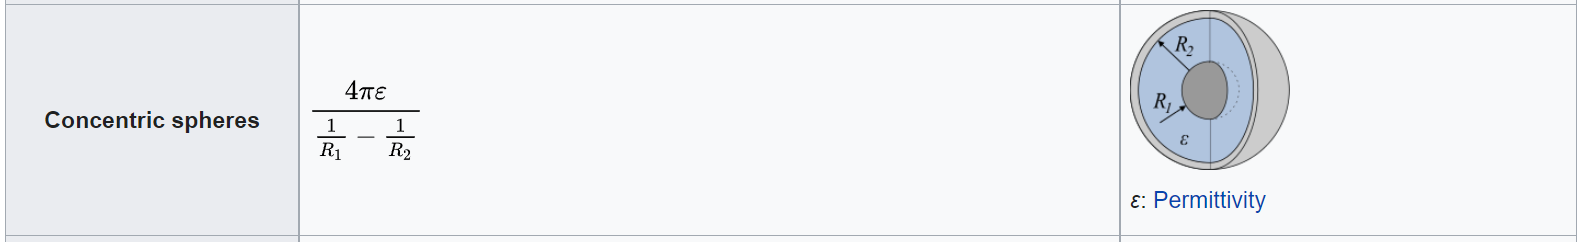
\includegraphics[width=.6\textwidth]{figures/cavity_capacitance.png}
\end{figure}
\begin{itemize}
    \item (Cavity Signal Manifold) 
    
        \begin{itemize}
            \item (AC Cavity) Let $M=N^3 \times T$ where $N^3$ is the cavity and $T$ is a signal. \colin{It would be interesting to combine both of these $T$? And earlier it would be good to work with them a bit. Will it be possible to show that $e_0^2=-1$ must be true? \url{https://math.stackexchange.com/questions/2542841/de-rham-cohomology-of-s1}}. We then have that 
\begin{equation}
    \partial M = \partial N^3 \times S^1
\end{equation}
since $\partial S^1 = \emptyset$. The homology for $S^1$ is then $H_0(S^1)\cong \R$, $H_1(S^1)\cong 0$, and for $k\geq 2$, $H_k(S^1)\cong 0$. We can now use the K\"unneth formula to find
\begin{align}
    H^k(M) &\cong \bigoplus_{i+j=k} H^i(N^3)\otimes H^j(S^1)\\
    H^k(\boundary) &\cong \bigoplus_{i+j=k} H^i(\partial N^3)\otimes H^j(S^1)\\
    H^k(M,\boundary) &\cong \bigoplus_{i+j=k} H^i(N^3,\partial N^3)\otimes H^j(S^1)
\end{align}
So we get the following (omitting those that are zero):
\begin{align*}
    H^0(M) &\cong \underbrace{\R \otimes \R}_{H^0(N^3)\otimes H^0(S^1)} \cong \R\\
    H^1(M) &\cong \underbrace{(\R \otimes \R)}_{H^0(N^3)\otimes H^1(S^1)} \oplus \underbrace{(0 \otimes \R)}_{H^1(N^3)\otimes H^0(S^1)} \cong \R\\
    H^2(M) &\cong \underbrace{(\R \otimes 0)}_{H^0(N^3)\otimes H^2(S^1)} \oplus \underbrace{(0 \otimes \R)}_{H^1(N^3)\otimes H^1(S^1)} \oplus \underbrace{(\R \otimes \R)}_{H^2(N^3)\otimes H^0(S^1)} \cong \R\\
    H^3(M) &\cong \underbrace{(\R \otimes 0)}_{H^0(N^3)\otimes H^3(S^1)} \oplus \underbrace{(0 \otimes 0)}_{H^1(N^3)\otimes H^2(S^1)} \oplus \underbrace{(\R \otimes \R)}_{H^2(N^3)\otimes H^1(S^1)} \oplus \underbrace{(0 \otimes \R)}_{H^3(N^3)\otimes H^0(S^1)} \cong \R\\
\end{align*}
hence on $M$ a nontrivial class $H^1(M)$ is generated by a vector field of the form $\epsilon e_0$ where $e_0$ is the generator of the nontrivial homology class of $S^1$ and $\rho$ is a constant scalar. In $H^2(M)$ we have a nontrivial class given by $q E$ where $q$ is a scalar and $E$ is an absolute second homology class (a generator can be given by $\frac{1}{r^2}e_\theta e_\phi$). Finally, the nontrivial class in $H^3(M)$ proves most interesting since we can put $E\wedge e_0$.
\begin{align*}
    H^0(\partial M) &\cong \underbrace{\R^2 \otimes \R}_{H^0(\partial N^3)\otimes H^0(S^1)} \cong \R^2 \\
    H^1(\partial M) &\cong \underbrace{(\R^2 \otimes \R)}_{H^0(\partial N^3)\otimes H^1(S^1)} \oplus \underbrace{(0 \otimes \R)}_{H^1(\partial N^3)\otimes H^0(S^1)} \cong \R^2 \\
    H^2(\partial M) &\cong \underbrace{(\R \otimes 0)}_{H^0(\partial N^3)\otimes H^2(S^1)} \oplus \underbrace{(0 \otimes \R)}_{H^1(\partial N^3)\otimes H^1(S^1)} \oplus \underbrace{(\R^2 \otimes \R)}_{H^2(\partial N^3)\otimes H^0(S^1)} \cong \R^2\\
    H^3(\partial M) &\cong \underbrace{(\R^2 \otimes 0)}_{H^0(\partial N^3)\otimes H^3(S^1)} \oplus \underbrace{(0 \otimes 0)}_{H^1(\partial N^3)\otimes H^2(S^1)} \oplus \underbrace{(\R^2 \otimes \R)}_{H^2(\partial N^3)\otimes H^1(S^1)} \oplus \underbrace{(0 \otimes \R)}_{H^3(\partial N^3)\otimes H^0(S^1)} \cong \R^2\\
\end{align*}
By Poincare duality it suffices to mention just $H^0$ and $H^1$. There are two constants to be defined for building the two classes of $H^0(\partial M)$, namely $\epsilon q_0$ and $\epsilon q_1$ for the inner and outer spheres respectively. In $H^1(\partial M)$ we have the classes $V_0 e_0$ and $V_1 e_0$
\begin{align*}
    H^1(M,\partial M) &\cong \underbrace{(0 \otimes \R)}_{H^0(N^3,\partial N^3)\otimes H^1(S^1)} \oplus \underbrace{(\R \otimes \R)}_{H^1(N^3,\partial N^3)\otimes H^0(S^1)} \cong \R \\
    H^2(M,\partial M) &\cong \underbrace{(0 \otimes 0)}_{H^0(N^3,\partial N^3)\otimes H^2(S^1)} \oplus \underbrace{(\R \otimes \R)}_{H^1(N^3,\partial N^3)\otimes H^1(S^1)} \oplus \underbrace{(0 \otimes \R)}_{H^2(N^3,\partial N^3)\otimes H^0(S^1)} \cong \R\\
    H_3(M,\partial M) &\cong \underbrace{(0 \otimes 0)}_{H^0(N^3,\partial N^3)\otimes H^3(S^1)} \oplus \underbrace{(\R \otimes 0)}_{H^1(N^3,\partial N^3)\otimes H^2(S^1)} \oplus \underbrace{(0 \otimes \R)}_{H^2(N^3,\partial N^3)\otimes H^1(S^1)} \oplus \underbrace{(\R \otimes \R)}_{H^3(\partial N^3)\otimes H^0(S^1)} \cong \R\\
    H_4(M,\partial M) &\cong \underbrace{(0 \otimes 0)}_{H^0(N^3,\partial N^3)\otimes H^4(S^1)} \oplus \underbrace{(\R \otimes 0)}_{H^1(\partial N^3)\otimes H^3(S^1)} \oplus \underbrace{(0 \otimes 0)}_{H^2(N^3,\partial N^3)\otimes H^2(S^1)} \oplus \underbrace{(\R \otimes \R)}_{H^3(N^3,\partial N^3)\otimes H^1(S^1)} \oplus \underbrace{(0 \otimes \R)}_{H^4(N^3,\partial N^3)\otimes H^0(S^1)} \cong \R.
\end{align*}
These above are all granted by Poincar\'e--Lefschetz but it is worth mentioning the $H^2(M)$ class is captured in the $H^2(M,\partial M)$ class by $\epsilon E = \frac{\rho}{r^2} e_r$ since $\grad \wedge E=0$ and $\normal \wedge E=0$. \colin{We can actually just do Hodge theory on both parts}

Finally the long exact sequence of homology
\[
\begin{tikzcd}
0 \arrow[r]                          & H_4(\partial M)\cong 0 \arrow[r, "\iota^*"]            & H_4(M)\cong 0 \arrow[r, "\jmath^*"]          & {H_4(M,\partial M)\cong \R} \arrow[r, "\partial"]          & \cdots \\
\cdots \arrow[r, "\partial"]                          & H_3(\partial M)\cong \R^2 \arrow[r, "\iota^*"]            & H_3(M)\cong \R \arrow[r, "\jmath^*"]          & {H_3(M,\partial M)\cong \R} \arrow[r, "\partial"]          & \cdots \\
\cdots \arrow[r, "\partial"] & H_2(\partial M)\cong \mathbb{R}^2 \arrow[r, "\iota^*"]   & H_2(M) \cong \R \arrow[r, "\jmath^*"]         & {H_2(M,\partial M)\cong \R} \arrow[r, "\partial"] & \cdots \\
\cdots \arrow[r, "\partial"] & H_1(\partial M)\cong \mathbb{R}^2 \arrow[r, "\iota^*"] & H_1(M)\cong \mathbb{R} \arrow[r, "\jmath^*"] & {H_1(M,\partial M)\cong\R} \arrow[r, "\partial"]          & \cdots \\
\cdots \arrow[r, "\partial"] & H_0(\partial M)\cong \mathbb{R}^2 \arrow[r, "\iota^*"]   & H_0(M)\cong \mathbb{R} \arrow[r, "\jmath^*"] & {H_0(M,\partial M)\cong 0} \arrow[r, "\partial"]          & 0     
\end{tikzcd}
\]
\colin{I want to get the AC behavior of a capacitor out of this just from topology. Not sure if it is actually possible. Could also treat this like a resistor.}

            \item (DC Cavity) Let $M=N^3 \times T$ where $N^3$ is the cavity and $T=[0,\infty]$ is a DC signal \colin{Okay this is annoying. Probably just use $[0,\infty)$ and look at compactly supported homology}. We then have that 
\begin{equation}
    \partial M = \partial N^3 \times T \cup N^3 \times \{0,1\} \cup \partial N^3 \times \{\infty\} = (N^3 \times T) \cup (\partial N^3 \sqcup \partial N^3)
\end{equation}
since $\partial [0,\infty]$. 
\begin{align}
    H^k(M) &\cong \bigoplus_{i+j=k} H^i(N^3)\otimes H^j(T)\\
    H^k(\boundary) &\cong H^k(\partial N^3) \oplus H^k(\partial N^3)\\
    H^k(M,\boundary) &\cong \bigoplus_{i+j=k} H^i(N^3,\partial N^3)\otimes H^j(T,\partial T)
\end{align}
Noting that the cohomology of a disjoint union $\sqcup$ is the sum of cohomologies. 

So we get the following (omitting those that are zero):
\begin{align*}
    H^0(M) &\cong \underbrace{\R \otimes \R}_{H^0(N^3)\otimes H^0(T)} \cong \R\\
    H^1(M) &\cong \underbrace{(\R \otimes 0)}_{H^0(N^3)\otimes H^1(T)} \oplus \underbrace{(0 \otimes \R)}_{H^1(N^3)\otimes H^0(T)} \cong 0\\
    H^2(M) &\cong \underbrace{(\R \otimes 0)}_{H^0(N^3)\otimes H^2(T)} \oplus \underbrace{(0 \otimes 0)}_{H^1(N^3)\otimes H^1(T)} \oplus \underbrace{(\R \otimes \R)}_{H^2(N^3)\otimes H^0(T)} \cong \R\\
    H^3(M) &\cong \underbrace{(\R \otimes 0)}_{H^0(N^3)\otimes H^3(T)} \oplus \underbrace{(0 \otimes 0)}_{H^1(N^3)\otimes H^2(T)} \oplus \underbrace{(\R \otimes 0)}_{H^2(N^3)\otimes H^1(T} \oplus \underbrace{(0 \otimes \R)}_{H^3(N^3)\otimes H^0(T)} \cong 0\\
\end{align*}
\colin{Redo this paragraph for DC}
hence on $M$ a nontrivial class $H^1(M)$ is generated by a vector field of the form $\rho e_0$ where $e_0$ is the generator of the nontrivial homology class of $S^1$ and $\rho$ is a constant scalar. In $H^2(M)$ we have a nontrivial class given by $\rho E$ where $\epsilon$ is a scalar and $J$ is an absolute second homology class (a generator can be given by $\frac{1}{r^2}e_\theta e_\phi$). Finally, the nontrivial class in $H^3(M)$ proves most interesting since we can put $E\wedge e_0$.
\begin{align*}
    H^0(\partial M) &\cong \underbrace{\R^2 \otimes \R}_{H^0(\partial N^3)\otimes H^0(S^1)} \cong \R^2 \\
    H^1(\partial M) &\cong \underbrace{(\R^2 \otimes \R)}_{H^0(\partial N^3)\otimes H^1(S^1)} \oplus \underbrace{(0 \otimes \R)}_{H^1(\partial N^3)\otimes H^0(S^1)} \cong \R^2 \\
    H^2(\partial M) &\cong \underbrace{(\R \otimes 0)}_{H^0(\partial N^3)\otimes H^2(S^1)} \oplus \underbrace{(0 \otimes \R)}_{H^1(\partial N^3)\otimes H^1(S^1)} \oplus \underbrace{(\R^2 \otimes \R)}_{H^2(\partial N^3)\otimes H^0(S^1)} \cong \R^2\\
    H^3(\partial M) &\cong \underbrace{(\R^2 \otimes 0)}_{H^0(\partial N^3)\otimes H^3(S^1)} \oplus \underbrace{(0 \otimes 0)}_{H^1(\partial N^3)\otimes H^2(S^1)} \oplus \underbrace{(\R^2 \otimes \R)}_{H^2(\partial N^3)\otimes H^1(S^1)} \oplus \underbrace{(0 \otimes \R)}_{H^3(\partial N^3)\otimes H^0(S^1)} \cong \R^2\\
\end{align*}
By Poincare duality it suffices to mention just $H^0$ and $H^1$. There are two constants to be defined for building the two classes of $H^0(\partial M)$, namely $\epsilon \rho_0$ and $\epsilon \rho_1$ for the inner and outer spheres respectively. In $H^1(\partial M)$ we have the classes $V_0 e_0$ and $V_1 e_0$
\begin{align*}
    H^1(M,\partial M) &\cong \underbrace{(0 \otimes \R)}_{H^0(N^3,\partial N^3)\otimes H^1(S^1)} \oplus \underbrace{(\R \otimes \R)}_{H^1(N^3,\partial N^3)\otimes H^0(S^1)} \cong \R \\
    H^2(M,\partial M) &\cong \underbrace{(0 \otimes 0)}_{H^0(N^3,\partial N^3)\otimes H^2(S^1)} \oplus \underbrace{(\R \otimes \R)}_{H^1(N^3,\partial N^3)\otimes H^1(S^1)} \oplus \underbrace{(0 \otimes \R)}_{H^2(N^3,\partial N^3)\otimes H^0(S^1)} \cong \R\\
    H_3(M,\partial M) &\cong \underbrace{(0 \otimes 0)}_{H^0(N^3,\partial N^3)\otimes H^3(S^1)} \oplus \underbrace{(\R \otimes 0)}_{H^1(N^3,\partial N^3)\otimes H^2(S^1)} \oplus \underbrace{(0 \otimes \R)}_{H^2(N^3,\partial N^3)\otimes H^1(S^1)} \oplus \underbrace{(\R \otimes \R)}_{H^3(\partial N^3)\otimes H^0(S^1)} \cong \R\\
    H_4(M,\partial M) &\cong \underbrace{(0 \otimes 0)}_{H^0(N^3,\partial N^3)\otimes H^4(S^1)} \oplus \underbrace{(\R \otimes 0)}_{H^1(\partial N^3)\otimes H^3(S^1)} \oplus \underbrace{(0 \otimes 0)}_{H^2(N^3,\partial N^3)\otimes H^2(S^1)} \oplus \underbrace{(\R \otimes \R)}_{H^3(N^3,\partial N^3)\otimes H^1(S^1)} \oplus \underbrace{(0 \otimes \R)}_{H^4(N^3,\partial N^3)\otimes H^0(S^1)} \cong \R.
\end{align*}
These above are all granted by Poincar\'e--Lefschetz but it is worth mentioning the $H^2(M)$ class is captured in the $H^2(M,\partial M)$ class by $\epsilon E = \frac{\rho}{r^2} e_r$. \colin{We can actually just do Hodge theory on both parts. Maybe worth showing how this aligns with Poincare lefshetz?}
\colin{left off here}
Finally the long exact sequence of homology
\[
\begin{tikzcd}
0 \arrow[r]                          & H_4(\partial M)\cong 0 \arrow[r, "\iota^*"]            & H_4(M)\cong 0 \arrow[r, "\jmath^*"]          & {H_4(M,\partial M)\cong \R} \arrow[r, "\partial"]          & \cdots \\
\cdots \arrow[r, "\partial"]                          & H_3(\partial M)\cong \R^2 \arrow[r, "\iota^*"]            & H_3(M)\cong \R \arrow[r, "\jmath^*"]          & {H_3(M,\partial M)\cong \R} \arrow[r, "\partial"]          & \cdots \\
\cdots \arrow[r, "\partial"] & H_2(\partial M)\cong \mathbb{R}^2 \arrow[r, "\iota^*"]   & H_2(M) \cong \R \arrow[r, "\jmath^*"]         & {H_2(M,\partial M)\cong \R} \arrow[r, "\partial"] & \cdots \\
\cdots \arrow[r, "\partial"] & H_1(\partial M)\cong \mathbb{R}^2 \arrow[r, "\iota^*"] & H_1(M)\cong \mathbb{R} \arrow[r, "\jmath^*"] & {H_1(M,\partial M)\cong\R} \arrow[r, "\partial"]          & \cdots \\
\cdots \arrow[r, "\partial"] & H_0(\partial M)\cong \mathbb{R}^2 \arrow[r, "\iota^*"]   & H_0(M)\cong \mathbb{R} \arrow[r, "\jmath^*"] & {H_0(M,\partial M)\cong 0} \arrow[r, "\partial"]          & 0     
\end{tikzcd}
\]
\colin{I want to get the DC behavior of a capacitor out of this just from topology or just treat it like a resistor.}
\colin{Also do alexander duality}
        \end{itemize}





\item Let $N^3$ be the solid torus from before and let us consider the 4-manifold $M=N^3 \times S^1$. Note that this manifold admits global coordinates $(x,y,z,t)$ where $t$ is the angular coordinate on $S^1$. Moreover, $M$ is metrizable with a semi-Riemannian metric of signature $(+,+,+,-)$. In other words, $M$ is a valid spacetime. 
\colin{I think on a general spacetime foliated manifold, the Dirac operator restricted to the spatial leaves of the foliation is still elliptic. Can this be leveraged into something? Something like a time varying Hodge theory?}

We then have that 
\begin{equation}
    \partial M = \partial N^3 \times S^1
\end{equation}
since $\partial S^1 = \emptyset$. The homology for $S^1$ is then $H_0(S^1)\cong \R$, $H_1(S^1)\cong 0$, and for $k\geq 2$, $H_k(S^1)\cong 0$. We can now use the K\"unneth theorem to see that
\begin{equation}
    \bigoplus_{i+j=k} H_i(N^3)\otimes H_j(S^1) \cong H_k(M).
\end{equation}
So we get
\begin{align*}
    H_0(M) &\cong \underbrace{\R \otimes \R}_{H_0(N^3)\otimes H_0(S^1)} \cong \R\\
    H_1(M) &\cong \underbrace{(\R \otimes \R)}_{H_0(N^3)\otimes H_1(S^1)} \oplus \underbrace{(\R \otimes \R)}_{H_1(N^3)\otimes H_0(S^1)} \cong \R^2\\
    H_2(M) &\cong \underbrace{(\R \otimes 0)}_{H_0(N^3)\otimes H_2(S^1)} \oplus \underbrace{(\R \otimes \R)}_{H_1(N^3)\otimes H_1(S^1)} \oplus \underbrace{(0 \otimes \R)}_{H_2(N^3)\otimes H_0(S^1)} \cong \R\\
    H_3(M) &\cong \underbrace{(\R \otimes 0)}_{H_0(N^3)\otimes H_3(S^1)} \oplus \underbrace{(\R \otimes 0)}_{H_1(N^3)\otimes H_2(S^1)} \oplus \underbrace{(0 \otimes \R)}_{H_2(N^3)\otimes H_1(S^1)} \oplus \underbrace{(0 \otimes \R)}_{H_3(N^3)\otimes H_0(S^1)} \cong \R\\
    H_4(M) &\cong \underbrace{(\R \otimes 0)}_{H_0(N^3)\otimes H_4(S^1)} \oplus \underbrace{(\R \otimes 0)}_{H_1(N^3)\otimes H_3(S^1)} \oplus \underbrace{(0 \otimes 0)}_{H_2(N^3)\otimes H_2(S^1)} \oplus \underbrace{(0 \otimes \R)}_{H_3(N^3)\otimes H_1(S^1)} \oplus \underbrace{(0 \otimes \R)}_{H_4(N^3)\otimes H_0(S^1)} \cong 0
\end{align*}
\colin{In $H_3(M)$ I think this corresponds to Faraday's law (in a vacuum?) somehow. This is also seemingly the only ``interesting'' case in here. The rest all come from scalar functions in some way. Please read this comment with a hefty grain of salt}
and similarly 
\begin{align*}
    H_0(\partial M) &\cong \underbrace{\R \otimes \R}_{H_0(\partial N^3)\otimes H_0(S^1)} \cong \R \\
    H_1(\partial M) &\cong \underbrace{(\R \otimes \R)}_{H_0(\partial N^3)\otimes H_1(S^1)} \oplus \underbrace{(\R^2 \otimes \R)}_{H_1(\partial N^3)\otimes H_0(S^1)} \cong \R^3 \\
    H_2(\partial M) &\cong \underbrace{(\R \otimes 0)}_{H_0(\partial N^3)\otimes H_2(S^1)} \oplus \underbrace{(\R^2 \otimes \R)}_{H_1(\partial N^3)\otimes H_1(S^1)} \oplus \underbrace{(\R \otimes \R)}_{H_2(\partial N^3)\otimes H_0(S^1)} \cong \R^3\\
    H_3(\partial M) &\cong \underbrace{(\R \otimes 0)}_{H_0(\partial N^3)\otimes H_3(S^1)} \oplus \underbrace{(\R^2 \otimes 0)}_{H_1(\partial N^3)\otimes H_2(S^1)} \oplus \underbrace{(\R \otimes \R)}_{H_2(\partial N^3)\otimes H_1(S^1)} \oplus \underbrace{(0 \otimes \R)}_{H_3(\partial N^3)\otimes H_0(S^1)} \cong \R\\
    H_4(\partial M) &\cong \underbrace{(\R \otimes 0)}_{H_0(\partial N^3)\otimes H_4(S^1)} \oplus \underbrace{(\R^2 \otimes 0)}_{H_1(\partial N^3)\otimes H_3(S^1)} \oplus \underbrace{(\R \otimes 0)}_{H_2(\partial N^3)\otimes H_2(S^1)} \oplus \underbrace{(0 \otimes \R)}_{H_3(\partial N^3)\otimes H_1(S^1)} \oplus \underbrace{(0 \otimes \R)}_{H_4(\partial N^3)\otimes H_0(S^1)} \cong 0.
\end{align*}
\colin{Not only does the kunneth formula tell us where solutions may come from, it also tells us where we are killing them off.}
\[
\begin{tikzcd}
0 \arrow[r]                          & H_4(\partial M)\cong 0 \arrow[r, "\iota^*"]            & H_4(M)\cong 0 \arrow[r, "\jmath^*"]          & {H_4(M,\partial M)\cong \R} \arrow[r, "\partial"]          & \cdots \\
\cdots \arrow[r, "\partial"]                          & H_3(\partial M)\cong \R \arrow[r, "\iota^*"]            & H_3(M)\cong \R \arrow[r, "\jmath^*"]          & {H_3(M,\partial M)\cong \textcolor{red}{????}} \arrow[r, "\partial"]          & \cdots \\
\cdots \arrow[r, "\partial"] & H_2(\partial M)\cong \mathbb{R}^3 \arrow[r, "\iota^*"]   & H_2(M) \cong \R \arrow[r, "\jmath^*"]         & {H_2(M,\partial M)\cong \textcolor{red}{????}} \arrow[r, "\partial"] & \cdots \\
\cdots \arrow[r, "\partial"] & H_1(\partial M)\cong \mathbb{R}^3 \arrow[r, "\iota^*"] & H_1(M)\cong \mathbb{R}^2 \arrow[r, "\jmath^*"] & {H_1(M,\partial M)\cong\textcolor{red}{????}} \arrow[r, "\partial"]          & \cdots \\
\cdots \arrow[r, "\partial"] & H_0(\partial M)\cong \mathbb{R} \arrow[r, "\iota^*"]   & H_0(M)\cong \mathbb{R} \arrow[r, "\jmath^*"] & {H_0(M,\partial M)\cong \textcolor{red}{????}} \arrow[r, "\partial"]          & 0     
\end{tikzcd}
\]
\colin{Honestly $\partial$ is really just $\partial$ so I should stop that}
\end{itemize}


\end{example}







\subsection{Homotopy invariance}


%---------------------------------------------------------------------------------------------------------------------------
\subsection{Maxwell' Equations}
\colin{I want to do now build from the example before and integrate analysis. Specifically, it would be good to relate differential laws to integral laws by integration over loops and spheres and what not. This is where I think it will be pertinent to lay out maxwell's equations! The space time split should somehow correspond to the Kunneth theorem. I mean, the Clifford algebra is just a quotient of tensors.}

\colin{I am putting this after currents now because I think the conservation laws are THE way to derive this.}

For this example, let $M$ be a Lorentz 4-manifold and for simplicity assume $M$ supports global coordinates. Moreover, take the Minkwoski metric $\eta$ and assume that each $\G_xM = \clifford(T_xM,\eta)$ so we can put $\G_xM\cong \G_{1,3}$. We let the set of multivector fields on $M$ be given by $\G_{1,3}(M)$ to mimic our earlier example. 

Due to this metric signature, it will be pertinent to factor the Hodge-Dirac operator by
\begin{equation}
    \grad = \vect + \vecgrad
\end{equation}
and we refer to $\vect$ as the \emph{temporal gradient} and $\vecgrad$ as the \emph{spatial gradient} and define them as
\begin{align}
    \vect \coloneqq \blade{e}^0 \nabla_{\blade{e}_0} \qquad \textrm{and} \qquad \vecgrad \coloneqq \sum_{i=1}^3 \blade{e}^i \nabla_{\blade{e}_i}.
\end{align}
The notation will become clear momentarily. 

Let $F\in \G^2_{1,3}(M)$, then we can be split into constituent bivectors $E$ and $B$ by
\begin{align}
	F = E+B.
\end{align}
where
\begin{equation}
    E \coloneqq E^1 \blade{e}_0 \blade{e}_1 + E^2 \blade{e}_0 \blade{e}_2 + E^3 \blade{e}_0 \blade{e}_3 \qquad \textrm{and} \qquad B \coloneqq B^{3} \blade{e}_1 \blade{e}_2 + B^{2} \blade{e}_3 \blade{e}_1 + B^{1} \blade{e}_2 \blade{e}_3.
\end{equation}
As mentioned, this $F$ cannot in general be written as the wedge of two vector fields. Visually, this is because there are 2-dimensional subspaces in $\R^4$ that meet only in a point. For instance, the purely spatial subspace $\blade{E}_{23}$ meets the spatio-temporal subspace $\blade{E}_{01}$ only at the origin. This leads to a dramatic difference in how we would percieve the physics of bivector fields. Of course, we know the physical differences between $E$ and $B$.

If we apply the Hodge-Dirac operator to $F$ we get $\grad F = \grad \wedge F + \grad \contract F$ \colin{It would be interesting to see if $F$ links with $J = \grad \contract F$}. The grade-3 components are
\begin{align}
\label{eq:gauss_faraday}
	\grad \wedge F ~\implies~ \underbrace{\vecgrad \wedge B}_{\textrm{spatial}} + \underbrace{\vecgrad \wedge E + \vect \wedge B}_{\textrm{spatio-temporal}}.
\end{align}
Notice that we split these into components that are purely spatial and those that are spatio-temporal. If we force $\grad \wedge F=0$, then we find
\begin{align}
    \vecgrad \wedge B &= 0 &&\textrm{Gauss's law for magnetism}\\
    \vecgrad \wedge E + \vect \wedge B &= 0 &&\textrm{Faraday's law of induction.}
\end{align}
Notice that these are both homogeneous expressions since we took $\grad \wedge F=0$. To see this more explicitly, let $\blade{E}_{123}$ be the spatial trivector, then we can use this as the spatial dual by 
\begin{equation}
    \vec{B}=B\blade{E}_{321}= B^1\blade{e}_1+B^2\blade{e}_2+B^3\blade{e}_3
\end{equation}
and so we find that $\vecgrad \wedge B=0$ is equivalent to
\begin{equation}
    \vecgrad \cdot \vec{B}=0,
\end{equation}
which we recognize.

In 3 dimensions we have the cross product. It turns out we can write $\times$ between two spatial vectors $\blade{v},\blade{w}$ by
\begin{equation}
    \blade{v}\times \blade{w} = (\blade{v}\wedge \blade{w})\blade{E}_{321}.
\end{equation}
We can also define
\begin{equation}
    \vec{E}\coloneqq \blade{e}_0 \contract E = E^1 \blade{e}_1 + E^2 \blade{e}_2 + E^3 \blade{e}_3.
\end{equation}
Furthermore, if we identify $\frac{\partial}{\partial t}\coloneqq \nabla_{\blade{e}_0}=\blade{e}_0 \contract \vect$, then we can left contract Faraday's law by $\blade{e}_0$ and right multiply by $\blade{E}_{321}$ to get
\begin{equation}
    \vecgrad \times \vec{E} + \frac{\partial}{\partial t} \vec{B} = 0.
\end{equation}
Which is the more recognizable form of Faraday's law.

Onto the 
\begin{align}
\label{eq:spacetime_split}
	\grad \cdot F=\blade{J}~\implies~ \underbrace{\blade{e}^0 \cdot \vec{\grad} \cdot B = \blade{e}^0 \cdot \blade{J}}_{\textrm{spatial}} +  \underbrace{\blade{e}^0 \wedge (\vec{\boldsymbol{\partial_t}} \cdot E + \vec{\grad} \cdot E) = \blade{e}^0 \wedge \blade{J}}_{\textrm{spatio-temporal}}
\end{align}
are Gauss's law for electricity and Ampere's law respectively. Multiplication by $\blade{e}^0$ seen in \cref{eq:spacetime_split} is often called the spacetime split and since \cref{eq:gauss_faraday} is homogeneous, we do not see this as a necessary step. The equations for the electric and magnetic potential can be found this way as well.


$\grad F = \blade{J}$ or, as is typical
\begin{align}
	\grad \wedge F &= 0  &&\textrm{(homogeneous)}\\
	\grad \cdot F &= \blade{J} && \textrm{(inhomogeneous)}.
\end{align}
The equation $\grad F = \blade{J}$ is manifestly Lorentz invariant due to the spin invariance of $\grad$. \colin{Show the Lorentz transformation on $F$ and the $E$ and $B$ factors. That will be pertinent. Really only the lorentz boosts matter. I have stuff on this in my final report. Showing the reflections are invariants for $E$ but not $B$ would be cool, so that motivates why we need $Spin$ not $Pin$ and we have to use bivectors in $\mathfrak{spin}$.}

Supposing as well that $F$ has a potential $\blade{A}$, we can choose the Lorenz gauge so that $\grad \cdot \blade{A} = 0$ to get
\begin{equation}
\Delta \blade{A} = \blade{J}.
\end{equation}



% The space $\contfields{M}{\G}$ comes with the \emph{uniform norm}
% \begin{equation}
% \|f\|_\infty \coloneqq \sup_{x\in M} |f(x)|.
% \end{equation}
% Recall that at any point $x\in M$ we have that $|f(x)|^2=(f(x),f(x))$ is nothing but the Euclidean vector norm on $\R^{2n}$, so $\|f\|_\infty$ really is a norm on $\contfields{M}{\G}$. Furthermore:

% \begin{proposition}
% If $M$ is a compact Riemannian manifold, then the space $\contfields{M}{\G}$ is a Banach algebra.
% \end{proposition}
% \begin{proof}
% Note that $\G$ is a real $2^n$ dimensional Banach space with the multivector inner product. Since $M$ is a compact Hausdorff space, it follows that the space $\contfields{M}{\G}$ is a Banach space (see \cite{saab_integral_1990}). Taking $f,g \in \contfields{M}{\G}$ note that at each point
% \begin{align}
% (fg,fg) = \proj{}{(fg)^\dagger fg}=\proj{}{g^\dagger f^\dagger f g} = \proj{}{gg^\dagger f^\dagger f} = (gg^\dagger, f^\dagger f),
% \end{align}
% by the cyclic property (see \cite{chisolm_geometric_2012}). Using the Cauchy--Schwarz inequality
% \begin{align}
% |fg|^2 = (fg,fg) \leq (f^\dagger f, f^\dagger f) (gg^\dagger,gg^\dagger) = |f|^2 |g|^2.
% \end{align}
% Taking suprema, it follows that $\|fg\|_\infty\leq \|f\|_\infty\|g\|_\infty$.
% \end{proof}

% We topologize the Banach algebra $\contfields{M}{\G}$ with the uniform norm topology. Dually, we construct $\G$ valued functionals on this space which assume the name currents \emph{\`a la} de Rham.

\subsection{Currents of $k$-vectors}

To study the theory in application, we will focus on the two canonical notions of currents introduced before, namely the current of a $k$-vector and the current of a $k$-chain. We begin with the $k$-vector fields meaning that both homology and cohomology are Working solely with fields. This simplifies some of the computations but is arguably less geometrical in content. The geometric multiplication has two primary components to the product that are most important. This is the (left) interior product (or contraction) $\contract$ and the exterior product $\wedge$. We have already mentioned the wedge product is the cup product on the cohomology ring $H^\bullet(M)$, but we have yet to discuss the contraction. The dual map $\perp$ also plays a role in the relationships between $\wedge$ and $\contract$ and this extends nicely to homology and cohomology.

\subsubsection{Hodge Theory}

The study of fields leads us directly to Hodge theory which, more or less, uses analysis as a link to topology. Our notion of de Rham cohomology was built upon this. We took the cochain complex
\begin{equation}
\cdots \to \G^{k-1}(M) \xrightarrow{\grad \wedge_{k-1}} \G^k(M) \xrightarrow{\grad \wedge_{k}} \G^{k+1}(M) \to \cdots
\end{equation}
and defined the de Rham cohomology as $H^k_{\mathrm{dR}}(M)$ as the quotient $H^k_{\mathrm{dR}}(M) = \ker \grad \wedge_k ~ / ~ \im \grad \wedge_{k-1}$. But there exists a dual chain complex with the dual boundary map $\grad \contract$ given by
\begin{equation}
\cdots \to \G^{k-1}(M) \xleftarrow{\grad \contract_{k}} \G^k(M) \xleftarrow{\grad \contract_{k+1}} \G^{k+1}(M) \to \cdots
\end{equation}
\colin{In Schwarz they call this a cohomology}
If we take $H_k(M,\grad \contract)\coloneqq \ker \grad \contract_k ~ / ~ \im \grad \contract_{k+1}$, then we may ask about what relationships there between the above chain and cochain complex? Similarly, Hodge theory asks about the field structure of fields in homology classes that become most interesting in the case of manifolds with nonempty boundary. In that realm, we can solve elliptic boundary value problems which, perhaps unsurprisingly, are tied to topology.

\noindent \textbf{Monogenic Fields}

Given $M$ is a manifold with nonempty boundary $\partial M$, we can attempt to solve the following elliptic \colin{$\Delta$ isn't always elliptic, for example in spacetime} boundary value problem for a $k$-vector field. Let $\varphi \in \G(\partial M)$ then we wish to find $A \in \G(M)$ satisfying
\begin{equation}
    \label{eq:dirichlet_problem}
    \begin{cases}
    \Delta A = 0 & \textrm{in $\mathrm{int} M$}\\
    A\vert_{\partial M} = \varphi.
    \end{cases}
\end{equation}
In this case, we call $A$ \emph{harmonic} with boundary value $\varphi$ and $A$ exists uniquely for any $\varphi$ (see \cite[Theorem 3.4.6]{schwarz_hodge_1995} for a proof). In the case of electromagnetism, a harmonic $A_0 \in \G^0(M)$ corresponds to a vacuum solution for the scalar potential. To include source charges, we no longer solve a homogeneous expression (\emph{Laplace's equation} $\Delta A_0 = 0$) and would instead require $\Delta A_0 = \rho$ where $\rho$ is a distribution of charge. This inhomogeneous equation is often referred to as the \emph{Poisson equation}. In order to solve this problem, we must consider two boundary conditions. We have:
\begin{enumerate}[1.]
    \item the Dirichlet condition $\projection_{\pseudoscalar_{\partial}}(A)=0$. Also called the \emph{relative boundary conditions}.
    \item the Neumann condition $\projection_{\pseudoscalar_\partial}(A^\perp)=0$. Also called the \emph{absolute boundary conditions}.
\end{enumerate}
As a reminder, the map $\projection_{\pseudoscalar_\partial}$ acts as pointwise projection onto the tangent space to the boundary. In this sense, the Dirichlet condition forces the tangential component of the multivector field $A$ to vanish. The Neumann condition on $A$ is requires that $A$ has no components normal to the boundary\colin{I need to work out what this means on here}. These could, if need be, be imposed on $\grad \wedge A$ or $\grad \contract A$ as well. \cite[Proposition 1.2.6]{schwarz_hodge_1995} may be of insight.

Exploring solutions to the Poisson equation leads us to sub-problems. Recall that $\Delta = \grad^2$, then it may be just as illuminating to consider first order equations in terms of the Dirac operator $\grad$. The homogeneous equations turn out to carry a wealth of information with them.
\begin{definition}
Let $A \in \G(M)$, then we say $A$ is a \emph{monogenic} if $\grad A = 0$. We put $\monogenics(M)$ as the \emph{space of monogenic fields}.
\end{definition}
In the realm of Hodge theory, $k$-forms fields $\alpha_k \in \Omega^k(M)$ are called to be \emph{harmonic fields} if $(d+\delta)\alpha_k = 0$. The space of monogenic $k$-vector fields $\monogenics^k(M)$ is isomorphic to the space of $k$-forms that are harmonic fields. 

\begin{remark}
For $A_+\in \G^+(M)$ a spinor field, the equation $\grad A_+ = 0$ becomes a key point of study in Clifford analysis. The reason why is due to the grade mixing property of grad. For instance, if $M$ is dimension 2 and $g$ is positive definite, then if $A_+=A_0+A_2$ and $\grad A_+=0$ we have the Cauchy--Riemann equations
\begin{equation}
    \grad \wedge A_0 = \grad \contract A_2
\end{equation}
and $A_+$ is equivalent to a complex holomorphic function.
\end{remark}

\begin{definition}
The \emph{monogenic Dirichlet $k$-vector fields} are monogenic $k$-vector fields satisfying the Dirichlet condition
\begin{equation}
\monogenics_D^k(M) \coloneqq \{ A_k \in \G^k(M) ~\vert~ \grad A_k = 0, ~ \projection_{\pseudoscalar_{\partial}}(A)=0\}
\end{equation}
and the \emph{monogenic Neumann $k$-vector fields} are monogenic $k$-vector fields satisfying the Neumann condition
\begin{equation}
\monogenics_N^k(M) \coloneqq \{ A_k \in \G^k(M) ~\vert~ \grad A_k = 0, ~\projection_{\pseudoscalar_\partial}(A^\perp)=0 \}.
\end{equation}
\end{definition}

\subsubsection{Hodge Isomorphism and Hodge Duality}

This detour was taken to let us reach the following theorem.

\begin{theorem}[Hodge Isomorphisms]
When $g$ is definite (i.e., for Riemann manifolds) we have that $H^k(M) \cong \monogenics^k_N(M)$ and $H_k(M;\grad \contract) \cong \monogenics^k_D(M)$. Moreover $\monogenics^k_D(M) \cong H^k(M,\partial M)$.
\end{theorem}
For proof, see \cite[Theorem 2.6.1 and Corollary 2.6.2]{schwarz_hodge_1995}.

\begin{proposition}[Hodge Duality]
The (Hodge) dual $\perp$ is an isomorphism between $\monogenics^k_N(M)$ and $\monogenics^{n-k}_D(M)$. 
\end{proposition}
\begin{proof}
Let $A_k \in \monogenics^k_N(M)$ then $\grad A_k = 0$ and $\projection_{\pseudoscalar_\partial}(A_k^\perp)=0$. Applying $\perp$ we see
\begin{align}
    \grad A_k^\perp &= \grad \contract A_k^\perp + \grad \wedge A_k^\perp\\
        &= (\grad \wedge A_k)^\perp + (\grad \contract A_k)^\perp\\
        &=0
\end{align}
and similarly $\projection_{\pseudoscalar_\partial}(A_k^\perp)=0$ implies that the field $A_k^\perp$ satisfies the Dirichlet condition and hence $A_k^\perp \in \monogenics^{n-k}_D(M)$. 
\end{proof}

Moreover, using the Hodge isomorphisms (Hodge), the Hodge duality isomorphism ($\perp$), and the Poincar\'e-Lefschsetz (PL) duality isomorphism we have the following equivalences in the commutative diagram:
\[
% https://tikzcd.yichuanshen.de/#N4Igdg9gJgpgziAXAbVABwnAlgFyxMJZAJgBpiBdUkANwEMAbAVxiRAAkA9AawAoBZANwAlAJQgAvqXSZc+QigCs5KrUYs2XYGAC03CQNIAdI2joAnPIwAEQ62MnSQGbHgJEyAFlX1mrRBwA+tp6Bvyk1iZmllg2Qg5SMq7yRMre1L4aAeyBfOEJTi5y7kqkAAw+6v4gJgC2dDgAFgDGjMD8Epwh+oEAIgLiic6ybgok5ZV+bHUNLW0dPIEAcgOOScVjZaQAjJNZHDwCgiYARhAMUHAAnrVnDMAmYHQnDHQSkUYA7jBQAOYwg0KIxSKAA7Ds9tUtLp9EdTudLjc7g8jE8Xm8TAxzM0IOYwDBzINVD9-ggUKAAGbmCC1JBbEA4CBIADM1FeJxgDAACsCSiAGDAKTgQGysPi2FA6HBGj81iAqTSkGQGUzENtReKApLpbK2c9OTzknyxdhYCK1FMAiYcDAAB44cy1YAAEmEzusdGsFKwnKgEjlCtpiHpjKVGSq0yMNvtjuAXIAMv69RzubyFCATVgzUNA0h1SqWcmDWm2JmzeHLTUo3aHU6E-6c9SgyHVcoLftrTXY5yGFg0Hhmkn+frU0b02XWBrqlAIDgbVAA0289RQ4hPBWO9WY06e32B0P2cWx6WwKbJ-yxdPZ-PF4q1SvVeD29VhNYALwfepNE4nYDCKQfNGtbAFAr4ACoyriMC1AeI6GhsJ5nuavaaiA2oygujZ3i2SAAGxFqOCEBBO5qZC+76frMP5-gBnbbiB4GQeY0EHpeEpShhkgUBIQA
\begin{tikzcd}
                                  &  & \mathcal{M}^k_N(M)                                                                                                                                                                                &  &  & \mathcal{M}^{n-k}_D(M)                                                                                                                                                                        &  &                                         \\
H^k(M;\boldsymbol{\nabla} \wedge) &  &                                                                                                                                                                                                   &  &  &                                                                                                                                                                                               &  & H^{n-k}(M;\boldsymbol{\nabla}\lrcorner) \\
                                  &  & H^k(M;R) \arrow[rrrdd, leftrightarrow, dashed] \arrow[dd,leftrightarrow, "\textrm{PL}" description] \arrow[uu, leftrightarrow,"\textrm{elliptic}" description, dotted] \arrow[llu, leftrightarrow,"{R = \mathbb{R}, \textrm{dR Theorem}}" description, dashed] &  &  & {H^{n-k}(M,\partial M; R)} \arrow[dd, leftrightarrow,"\textrm{PL}" description] \arrow[uu, leftrightarrow,"\textrm{elliptic}" description, dotted] \arrow[rru, leftrightarrow,"{R = \mathbb{R}, \textrm{dR Theorem}}" description, dashed] &  &                                         \\
                                  &  &                                                                                                                                                                                                   &  &  &                                                                                                                                                                                               &  &                                         \\
                                  &  & {H_{n-k}(M, \partial M;R)} \arrow[rrruu,leftrightarrow, "\textrm{$R$ a field}" description, dashed]                                                                                                              &  &  & {H_k(M,R)}                                                                                                                                                                                    &  &                                        
\end{tikzcd}
\]
\colin{Hodge star still takes you from $H^k(M;\grad \wedge)$ to $H^{n-k}(M;\grad \contract)$}

\textcolor{red}{I'm a bit confused. Current $J$ must flow in loops since $\grad \contract J=0$. In other words, $J$ is in $H_1(M)$ But, this diagram seems to suggest that $J$ would be in $H_1(M,\partial M)$. All the books I find seem to say this diagram is correct, but this doesn't make physical sense. This paper \url{http://neo-classical-physics.info/uploads/3/4/3/6/34363841/topological_electromagnetism.pdf} seems to suggest that the HOMOLOGY (not cohomology) of $\grad \contract$ is isomorphic to the absolute homology. At any rate, the above diagram should be modified to show $H^k(M;\grad \wedge ) \cong H^{n-k}(M;\grad \wedge)$ by the Hodge star. But also a current could flow between two regions of different charge as in the cavity example and that would be a relative class. Maybe I'm just confusing currents inside of conductors with the induced currents you would find outside them?}

\begin{remark}
Please do note that the above isomorphisms to the monogenic fields require the metric $g$ to be definite otherwise we lose the elliptic properties of $\grad$!
\end{remark}

\begin{definition}
\label{def:monogenic_field_dual_to_current}
The \emph{monogenic field $A_k$ dual to the homological current $A^k$} is given by the chain of isomorphisms $PL \circ Hodge \circ \perp$.
\end{definition}

The monogenic field $A_k$ dual to a homological current $A^k$ is given explicitly by taking a smooth oriented manifold $K$ in the homology class of $A^k$ with tangent pseudoscalar $\pseudoscalar_K$.
\begin{enumerate}[i.]
    \item If $A^k \in H_k(M)$ then $A_k\in \monogenics^k_N(M)$ where $(A_k,\pseudoscalar_K)>0$ (so $A_k$ is oriented along $K$ and $\|A_k\|=1$;
    \item If $A^k \in H_k(M,\partial M)$, then $A_k \in \monogenics^k_D(M)$ where $(A_k,\pseudoscalar_K)>0$ and $\|A_k\|=1$.
\end{enumerate}

\colin{This is probably worth talking about}
\begin{theorem}
\[
H^k(M,\partial M) = H^k_{cpt}(M\setminus \partial M)
\]
\end{theorem}

\begin{figure}
    \centering
    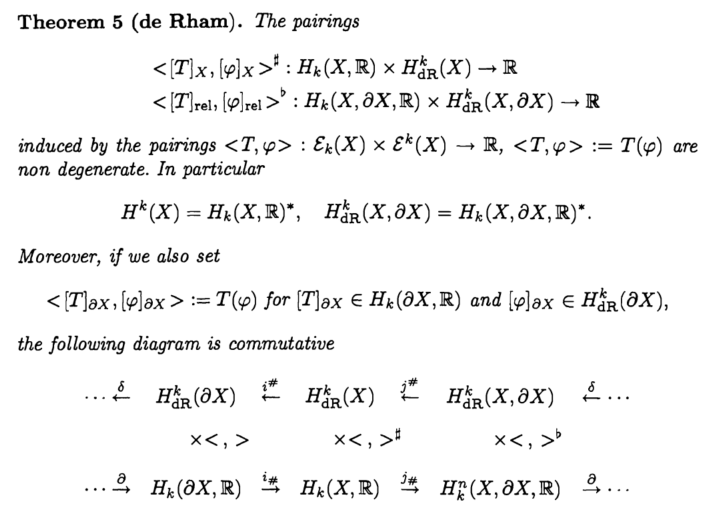
\includegraphics[width=.8\textwidth]{figures/de_rham_theorem.png}
    \caption{I think this figure goes to show that the perp maps above work even without Hodge theory.}
\end{figure}




\subsubsection{Periods}

A relevant question to ask about fields is whether a field is exact (i.e., in the image of $\grad \wedge$, or perhaps whether is is coexact (i.e., in the image of $\grad \contract$). When we constructed the de Rham cohomology, we took a look at the fields that were closed ($\grad \wedge f = 0$) and quotiented out by those that are exact $g = \grad \wedge h$. If the absolute cohomology $H^k(M)$ vanishes, then all closed $k$-vector fields are exact $k$-vector fields. 

A similar story is true for the coexact case. Recall that the homology $H_k(M;\grad \contract)\cong H^k(M,\partial M)$. To find $H_k(M;\grad \contract)$ we quotiented coclosed fields ($\grad \contract f = 0$) by the coexact fields ($g=\grad \contract h$) so if $H_k(M;\grad \contract)$ vanishes, all coclosed $k$-vector fields are coexact. By the Hodge isomorphisms, the same is true if the relative cohomology $H^k(M,\partial M)$ vanishes. 

By Poincar\'e--Lefschetz duality, the absolute and relative homology of $M$ tell the same story, just on currents with dual grade. All closed $k$-vector fields are exact if $H^k(M)\cong H_{n-k}(M,\partial M)$ vanish and all coclosed $k$-vector fields are coexact if $H^k(M, \partial M) \cong H_{n-k}(M)$ vanish.

\begin{example}
Consider two 3-manifolds the closed ball $\ball^3$ and the solid torus $S^1 \times \ball^2$. 
\begin{itemize}
    \item In $\ball^3$, if the curl of a vector field $\blade{E}$ vanishes, i.e, $\grad \wedge \blade{E}=0$, then it must be that $\blade{E}=\grad \wedge \phi$ for a scalar field $\phi\in \G^0(M)$. How do we know this?
    
    Note that $\ball^3$ has no relative or absolute homology other than $H_0(\ball^3)$ and $H_3(\ball)$, so all closed vector fields are exact. The typical theorem states that if for all closed curves (1-cycles) $\gamma \subset \ball^3$ if $\gamma(\blade{E})=0$, then $\blade{E}=\grad \wedge \phi$. \colin{These are theorem 6 and 7 on page 598 and 599 of giaquinta}. The pairing $\gamma(\blade{E})$ is invariant over homology classes of $\gamma$ \colin{Cite something} and since the only class is the trivial class, i.e., $[\gamma](\blade{E})=\gamma(\blade{E})$ it must be that $\gamma(\blade{E})=0$. In fact, this implies that $\gamma = \partial \Sigma$ where $\Sigma$ is a surface! \colin{This is theorem 7}
    
    \item In $S^1\times \ball^2$, this is no longer the case. Take the vector field $\blade{j}$ that constantly flows around the meridional direction of the solid torus. Then take a curve $\gamma$ that is an integral curve of this flow and it is clear that $\gamma(\blade{j})\neq 0$. Though $\blade{j}$ is closed, $\blade{j}$ is not exact. We see this since $H^1(M)$ does not vanish -- there are closed fields that are not exact. Dually, there exists nontrivial relative homology classes $H_2(M,\partial M)$ and these classes intersect with $\blade{j}$ \colin{We say this later}. Since $\blade{j}$ is constant it is also coclosed and moreover since $H_2(M)$ vanishes, it must be that $\blade{j}$ is coexact and $\blade{j}=\grad \contract B$ for $B\in \G^2(M)$. Since $H_1(M,\partial M)\cong 0$, all relative 1-cycles of the solid torus are in the trivial class and so for any $\gamma \in Z_1(M,\partial M)$, $\gamma(\blade{j})=0$. This means that $\gamma=B_1(M,\partial M)$ is a relative boundary a 2-chain. \colin{I don't think I have as good of an understanding of this example compared to the previous.}
\end{itemize}
\end{example}
The above work motivates the following definition.
\begin{definition}
Let $T_i^k \in Z_k(M)$ be a collection of closed $k$ currents (cycles) so that the homology classes $[T_i^k]$ are a basis for $H_k(M)$. Let $A_k \in Z^k(M)$ be a closed field, then the numbers
\begin{equation}
    T_i^k[A_k]
\end{equation}
are \emph{periods of the field $A_k$}. 
\end{definition}


The pairing between closed currents and closed forms captured through integration is a (co)homological invariant that has ramifications in analysis as follows. 
\begin{proposition}
\label{def:period}
For any closed $k$-vector $A_k$ and each co-closed $k$-current $B^k$, a the pairing $B^k[A_k]$ is invariant over both the homology class of $B^k$ and cohomology class of $A_k$.
\end{proposition}
\begin{proof}
Given closed $A_k$, exact $\partial \tilde{A}_{k-1}$, co-closed $B^k$, and co-exact $\grad \wedge \tilde{B}^{k-1}$
\begin{align}
(B^k+\partial \tilde{B}^{k-1})[A_k + \grad \wedge \tilde{A}_{k-1}] &= B^k[A_k]+B^k[\grad \wedge \tilde{A}_{k-1}]+\partial B^k[A_{k-1}]+\partial B^k[\grad \wedge \tilde{A}_{k-1}]\\
&= B^k[A_k] + \partial B^{k-1}[\tilde{A}_{k-1}] + B^k[\grad \wedge A_{k-1}]+\partial^2 B^{k-1}[\tilde{A}_{k-1}]\\
&=0.
\end{align}
\end{proof}
\begin{proposition}
\label{prop:periods}
    If all periods of a field $A_k$ vanish, then $A_k$ has a potential $\phi_{k-1}$ such that $\grad \wedge \phi_{k-1}=A_k$.
\end{proposition}
\colin{This appears in Hehl's text and probably elsewhere. It was also mostly used for the EM stuff which I'm not sure we want to include any of. Maybe it could fit in a Hodge section.}
We can see that the topology of the domain is intimately connected with solutions to certain partial differential equations. In the case that we are looking at locally star shaped regions, the Poincar\'e lemma guarantees a closed form is exact \cite[Proposition 5]{giaquinta_cartesian_1998}. If we worked with non-compactly supported multivectors we would have to take into account boundary conditions which adds many more complications \cite{schwarz_hodge_1995}.

How exactly should we think of this? In some sense, it seems that the Betti numbers of the manifold have an immediate impact on the solvability of the potential problem. Equivalently, homology rank seems to mark the failure of the fundamental theorem of calculus \colin{Tau says this}. 

Consider the solid torus, in this case there is one interesting class $H_1(M)$ other than the trivial class. It is clear that for the a representative of trivial class $[T_0^1][A_1]=0$ for any closed $A_1$. However, there are fields $A_1$ that are not gradients. The field that circulates through the torus will not vanish on the nontrivial class $[T_1^1][A_1]\neq 0$ and it is exactly the introduction of this homology class that prevents all such closed $A_1$ from being gradient fields. \colin{This is where Keenan Crane's illustration with Escher's staircase becomes pertinent}

\colin{This next arguments need more to be completely convincing}
Let $A_1$ be a closed vector field defined in a neighborhood of a point $x\in M \subset \R^3$, then let $\gamma_1$ be a closed curve encircling $x$ with radius $\epsilon$ and tangent to the plane $\bivector_{23}$, let $\gamma_2$ be the same but tangent to $\bivector_{31}$, and $\gamma_3$ be the same but in $\bivector_{12}$. Then \textcolor{red}{I claim}
\begin{equation}
\label{eq:local_def_for_curl}
    \grad \wedge A_1(x) = \lim_{\epsilon \to 0}  \left( \bivector_{23} \int_{\gamma_1} (A_1,\pseudoscalar_{\gamma_1})\mu_{\gamma_1} + \bivector_{31} \int_{\gamma_2} (A_1,\pseudoscalar_{\gamma_2})\mu_{\gamma_2} + \bivector_{12} \int_{\gamma_3} (A_1,\pseudoscalar_{\gamma_3})\mu_{\gamma_3} \right) 
\end{equation}
The intuition here is that the curl of a vector field is an infinitesimal circulation in some plane. So, it is true that if $\grad \wedge A_1=0$, then the above integrals all vanish, however, it becomes clear that the contrary statement that this implies $A_1 = \grad \wedge \phi_0$ is not guaranteed. Sure, if the only $H_1(M)$ class is trivial, then the only way is for all integrals over closed curves to be zero and that implies the curl is zero, but in the case where there is a nontrivial class, the integrals in \cref{eq:local_def_for_curl} will still vanish but we will not be able to solve the potential problem \colin{Again Escher's staircase is the visual}.

But the same is true for divergence. Let $A_2$ be a bivector field, and let $S$ be a sphere of radius $\epsilon$ encircling $x$, then the divergence
\begin{equation}
    \label{eq:local_def_for_div}
    \grad \wedge A_2(x) = \lim_{\epsilon \to 0} \int_S (A_2, \pseudoscalar_S) \mu_S = \lim_{\epsilon \to 0} \int_S (A_2^\perp,\normal_S)\mu_S
\end{equation}
so the divergence at a point is a flux through an infinitesimal sphere about that point. So, it is clear that if $\grad \wedge A_2=0$, then integrals over the trivial class in $H_2(M)$ all vanish. However, if there is a nontrivial $H_2(M)$ class, it is not clear that $A_2 = \grad \wedge \phi_1$.

\textcolor{red}{In fact, the infinitesimal limits require the curves/spheres to be in trivial homology classes since local neighborhoods are always trivial (convex even). The typical definition for these derivatives just does not take the other homology classes into account.}


\colin{I think you could probably define a gradient in this way, but it would basically just come down to finite differences essentially}

\subsubsection{Cap Product}

The contraction product $\contract$ on $\G(M)$ extends to a product on homology and cohomology. Typically, the cap product $\frown$ is a map $\frown \colon H^\ell(M) \times H_k(M) \to H_{k-\ell}(M)$ which pairs together a cohomology class with a homology class. It turns out that when thinking of homology and cohomology in terms of fields, the contraction is the cap product.

\begin{theorem}
\label{thm:cap}
Let $A_\ell \in H^\ell(M)$ and $B^k \in H_k(M)$. Then if $B_k$ is a $k$-vector field representative of the homology class of $B^k$, then $A_\ell \frown B^k = A_\ell \contract B_k$.
\end{theorem}
\begin{proof}
Take $A_\ell\in H^\ell(M)$ and $B^k \in H_k(M)$. Using the Hodge isomorphism, there exists a field $B_k \in \monogenics^k_N(M)$ representing $B^k \in H_k(M)$. We wish to show that $A_\ell \contract B_k \in H_{k-\ell}(M)$ which, by the Hodge isomorphisms again, means it suffices to show $A_\ell \contract B_k \in \monogenics^{k-\ell}_N(M)$. First,
\begin{align}
    \grad \contract (A_\ell \contract B_k) &= \grad \contract (A_\ell \wedge B_k^\perp)^\perp\\
    &= [\grad \wedge (A_\ell \wedge B_k^\perp)]^\perp\\
    &= [(\grad \wedge A_\ell)\wedge B_k^\perp +(-1)^\ell A_\ell \wedge (\grad \wedge B_k^\perp)]^\perp\\
    &= 0.
\end{align}
Next,
\begin{align}
    \grad \wedge (A_\ell \contract B_k) &= \grad \wedge (A_\ell \wedge B_k^\perp)^\perp\\
    &= (-1)^{(n-k)\ell}\grad \wedge (B_k^\perp \wedge A_\ell^\perp)\\
    &= (-1)^{(n-k)\ell}(\grad \wedge B_k^\perp)\wedge A_\ell^\perp +(-1)^{(n-k)(n-\ell)\ell} A_\ell^\perp \wedge (\grad \wedge B_k^\perp)\\
    &= 0.
\end{align}
Then we have
\begin{align}
    \projection_{\pseudoscalar_\partial}((A_\ell \contract B_k)^\perp)&= \projection_{\pseudoscalar_\partial}(A_\ell \wedge B_k^\perp)\\
    &=0,
\end{align}
since $\projection_{\pseudoscalar_\partial}(B_k^\perp)=0$ and the exterior product $A_\ell \wedge B_k^\perp$ must contain only multivectors that do not project onto $\pseudoscalar_\partial$.
\end{proof}

To see the action of the cap product on the level of currents, let $A_\ell \in \G^\ell(M)$ and $B_k \in \G^k(M)$ then $A_\ell \contract B_k$ is a $k-\ell$-vector field. Let $T^{k-\ell}$ be the current of the $k-\ell$-vector $A_\ell \contract B_k$ then
\begin{equation}
T^{k-\ell}[-] = \int_M (A_\ell \contract B_k, -)\mu.
\end{equation}
Take a $k-\ell-1$-vector $C_{k-\ell-1}$ and 
\begin{align}
    \partial T^{k-\ell}[C_{k-\ell-1}] &= \int_M (A_\ell \contract B_k, \grad \wedge C_{k-\ell-1})\mu\\
    &= \int_M (\grad \contract (A_\ell \contract B_k),C_{k-\ell-1})\mu + (-1)^p\int_{\partial M} \left((C_{k - \ell -1} \contract (A_\ell \contract B_k)^\dagger,\normal\right)\mu_\partial && \textrm{Green's formula}\\ 
    &= 0
\end{align}
since we have shown $\grad \contract (A_\ell \contract B_k)=0$ in the previous proof and since $B_k$ must have no components normal (meaning no blades with a $\normal$ in them) to $\partial M$ since it is a Neumann field we know the boundary integral vanishes.

\colin{I left off here for this section but it is worth mentioning the cap product can be extended to relative (co)homology using the dual}
For posterity, by letting $\ell = k$ we see that $X^0 = B^k \frown A_k = X^0 \in H_0(M)$ so that $X^0$ is a $0$-current, i.e., a collection of points $\partial X^0 = 0$ so that each $x\in X^0$\colin{This is probably horrific notation but I really think $X^0$ is really just a "discrete" set of points.}. For some smooth scalar field $C_0$,
\begin{equation}
X^0[C_0] = \sum_{x\in X} C_0(x).
\end{equation}
Since $B_0$ is closed, it is constant on each connected component. The cap product above leads us to an important duality theorem of the $\R$ homology and cohomology of smooth manifolds.



Poincar\'e duality essentially builds the isomorphism by using the cap product by taking the fundamental class $\delta_M$ and a $k$-form $\alpha_k \in H^k(M)$ to get the Poincar\'e dual $\overline{\alpha_k} \in H_{n-k}(M)$
\begin{equation}
\overline{\alpha_k} = (\delta_M \frown \alpha_k)[-] = \int_M (-,A_k \rfloor \blade{I})\mu
\end{equation}
which we see is well-defined since
\begin{align}
\partial \overline{\alpha_k}[\beta_{k-1}] = \int_M (B_{k-1}, \grad \cdot (A_k \rfloor \blade{I}))\mu = \int_M (B_{k-1},(\grad \wedge A_k)\blade{I}) \mu =0,
\end{align}
since $A_k$ is a closed $k$-vector field. It is a worthy remark to mention that the $(n-k)$-vector associated to $\overline{\alpha_k}$ is given by $A_k \rfloor \blade{I}$ which is often referred to as the dual and we can put $A_k^\perp = A_k \rfloor \blade{I}$. If we allow ourselves to work with distributional multivectors, then we can realize the cap product and Poincar\'e duality via typical multivector operations.
\colin{This is the poincare dual that Hatcher uses since we cap with the fundamental class. So it literally does align with the pseudoscalar dual.}

\subsubsection{Other products?}

From \cite{delphenich_axioms_2005} we also find that the Lie bracket gives a product structure on homology.
\begin{theorem}
The Lie bracket of vector fields is a map on the first homology classes
\[
[-,-] \colon H_1(M) \times H_1(M) \to H_1(M).
\]
\end{theorem}
\begin{proof}
Take $\blade{u}, \blade{v} \in H_1(M)$ as smooth vector fields, then 
\begin{align}
\grad \cdot [\blade{u},\blade{v}] &= \grad \cdot (\mathcal{L}_{\blade{u}} \blade{v})\\
&= \grad \cdot (\grad \wedge (\blade{u}\cdot \blade{v}) + \blade{u}\cdot (\grad \wedge \blade{v})) &&\textrm{by Cartan formula}\\
&= \grad \cdot \left( (\grad \wedge \blade{u})\wedge \blade{v}^\perp - \blade{u} \wedge (\grad \wedge \blade{v}^\perp) + \blade{u} \cdot (\grad \wedge \blade{v})\right)\\
&= \grad \cdot \left( (\grad \wedge \blade{u}) \wedge \blade{v}^\perp + \blade{u}\cdot (\grad \wedge \blade{v})\right) && \textrm{by Poincar\'e duality}\\
&= \grad \cdot \left( (\grad \wedge \blade{u}) \cdot \blade{v}\right)^\perp  + \grad \cdot \left( \blade{u} \cdot (\grad \wedge \blade{v} ) \right)\\
&= \left( \grad \wedge ((\grad \wedge \blade{u})\wedge \blade{v}^\perp)\right)^\perp +\left( \grad \wedge ((\grad \wedge \blade{v}) \wedge \blade{u}^\perp)\right)^\perp \\
&= (-1)^{n-1}\left( (\grad \wedge \blade{u})\wedge (\grad \wedge \blade{v}^\perp)\right)^\perp + (-1)^{n-1} \left( (\grad \wedge \blade{v}) \wedge (\grad \wedge \blade{u}^\perp)\right)^\perp\\
&= 0 && \textrm{by Poincar\'e duality}
\end{align}
\end{proof}
\colin{What about relative homology? I should double check this theorem is written correctly since I am using $\grad \cdot$ it may actually be a product on relative homology.}

\begin{proposition}
\textcolor{red}{Does the commutator product $\times$ give some map on second homology or cohomology classes?}
\end{proposition}


\colin{Giaquinta theorem 5 on page 598 looks good. The pairings for both absolute and relative homology are really used to prove a lot of stuff.}

\subsubsection{Poincar\'e Pairing and Intersection Homology}

\noindent \textbf{Poincar\'e pairing on cohomology}

The cap product is a product between homology and cohomology $\frown H^\ell(M) \times H_k(M) \to H_{k-\ell}(M)$, but by Poincar\'e--Lefschetz duality we expect that we can perhaps dualize this in some way. Moreover, \cref{eq:contract_dual,eq:wedge_dual}. For instance, in the case $k=\ell$ we have the isomorphism $H_k(M)\cong H^{n-k}(M,\partial M)$. Using our Hodge isomorphisms $H^k(M) \cong \monogenics^k_N(M)$ and $H^{n-k}(M,\partial M) \cong \monogenics^{n-k}_D(M)$. We then have the nondegenerate bilinear pairing (\cite[Theorem 3]{giaquinta_cartesian_1998-1}) for $A_k \in \monogenics^k_N(M)$ and $B_{n-k} \in \monogenics^{n-k}_D(M)$
\begin{equation}
M[ A_k \wedge B_{n-k}] = \int_M A_k \wedge B_{n-k} \contract d X_n
\end{equation}
where $M$ is the current for the $n$-chain $M$. But we can take the dual of $B_{n-k}^\perp = B_k \in \monogenics^k_{N}$ and note that
\begin{equation}
    M[A_k \wedge B_{n-k}] = M\left[(A_k \contract B_k)^\perp\right] = \int_M A_k \contract B_k \mu = \multivecinnerproduct{A_k}{B_k}.
\end{equation}
Of course, this extends to the pairing between Dirichlet harmonic fields too (just take the dual of $A_k$ before).

We see that $A_k \contract B_k \in H_0(M)$ is the cap product and so $(A_k \contract B_k)^\perp \in H^n(M,\partial M)$ and moreover we see the duality between the cap and cup product as $A_k \wedge B_k^\perp = (A_k \contract B_k)^\perp$ where $\wedge \colon H^k(M) \times H^{n-k}(M)\to H^n(M)$. Note that the top relative homology of a compact connected manifold is 1-dimensional so $H_n(M, \partial M)\cong \R$ in that case and it is given by the fundamental class $M$. 

\begin{proposition}
The multivector field inner product is invariant over cohomology.
\end{proposition}
\begin{proof}
Let $A_k, B_k \in H^k(M) \cong \monogenics^k_N(M)$, then
\begin{align}
    \multivecinnerproduct{A_k + \grad \wedge a_{k-1}}{B_k + \grad \wedge b_{k-1}} &= \multivecinnerproduct{A_k}{B_k} + \multivecinnerproduct{A_k}{\grad \wedge b_{k-1}} + \multivecinnerproduct{\grad \wedge a_k}{B_k} + \multivecinnerproduct{\grad \wedge a_k}{\grad \wedge b_k}.
\end{align}
The proof is by Green's formula since
\begin{align}
    \multivecinnerproduct{A_k}{\grad \wedge b_{k-1}} &= \int_M (A_k,\grad \wedge b_{k-1})\mu\\
    &= \int_M (\grad \contract A_k, b_{k-1})\mu + (-1)^p \int_{\partial M} (b_{k-1}\contract A_k,\normal)\mu_\partial 
\end{align}
where the first integral is zero since $\grad A_k = 0$ and the second since $\projection_{\pseudoscalar_\partial}(A^\perp)=0$. By the same logic, the terms $\multivecinnerproduct{\grad \wedge a_k}{B_k}$ and $\multivecinnerproduct{\grad \wedge a_k}{\grad \wedge b_k}$ vanish as well and
\begin{equation}
    \multivecinnerproduct{A_k + \grad \wedge a_{k-1}}{B_k + \grad \wedge b_{k-1}} = \multivecinnerproduct{A_k}{B_k}
\end{equation}
shows the intended result.
\end{proof}

\noindent \textbf{Intersection index on homology}

By applying Poincar\'e--Lefschets to the Poincar\'e pairing on cohomology, we get the \emph{intersection index} on homology. In particular $i(-,-)\colon H_k(M)\times H_{n-k}(M,\partial M) \to \R$. In particular, let $A^k \in H_k(M)$ and $B^{n-k} \in H_{n-k}(M,\partial M)$ with $A_k \in \monogenics^k_N(M)$ as the the $PL \circ Hodge \circ \perp$ isomorphism \colin{This is what I call the harmonic or monogenic mollification. But I don't think this name is that great. I also called this the monogenic field dual to the current in \cref{def:monogenic_field_dual_to_current}} and $B_{k} \in \monogenics^{k}_N(M)$ as the $PL \circ Hodge$ isomorphism of $B^k$. Then
\begin{equation}
    i(A^k, B^{n-k}) = \multivecinnerproduct{A_k}{B_k}.
\end{equation}

But, if we take the cap product $\wedge \colon H^k(M) \times H^\ell(M) \to H^{k+\ell}(M)$ we can dualize to a map
\begin{equation}
    \wedge^\perp \colon H_{n-k}(M,\partial M) \times H_{n-\ell}(M) \to H_{2n-k-\ell}
\end{equation}
That is, if $A_k \in H^k(M)$ and $B_\ell \in H^\ell(M)$ then $A_k \wedge B_\ell \in H^{k-\ell}(M)$. But taking $A_k^\perp$ and $B_\ell^\perp$ and
\begin{align}
    A_k^\perp \wedge B_\ell^\perp = (A_k^\perp \contract B_\ell)^\perp \in H_{2n-k-\ell}.
\end{align}
This just dualizes the first component of the cap product as seen in \cref{thm:cap}.

\colin{Add the stuff about Kronecker index on manifolds. Giaquinta page 606. Smooth manifolds are rectifiable so this should all be fine when talking about those.}


\section{Examples}

\textcolor{red}{It would also be good to take 3 manifolds and product with $N^3 \times [0,\infty]$ and you can look at the boundary here too. One is the start config, and the other would be the steady state. Also, accelerating charges and light would probably be good to get in this seeing as light is still a solution to $\grad F=0$.}

\begin{figure}[H]
    \centering
    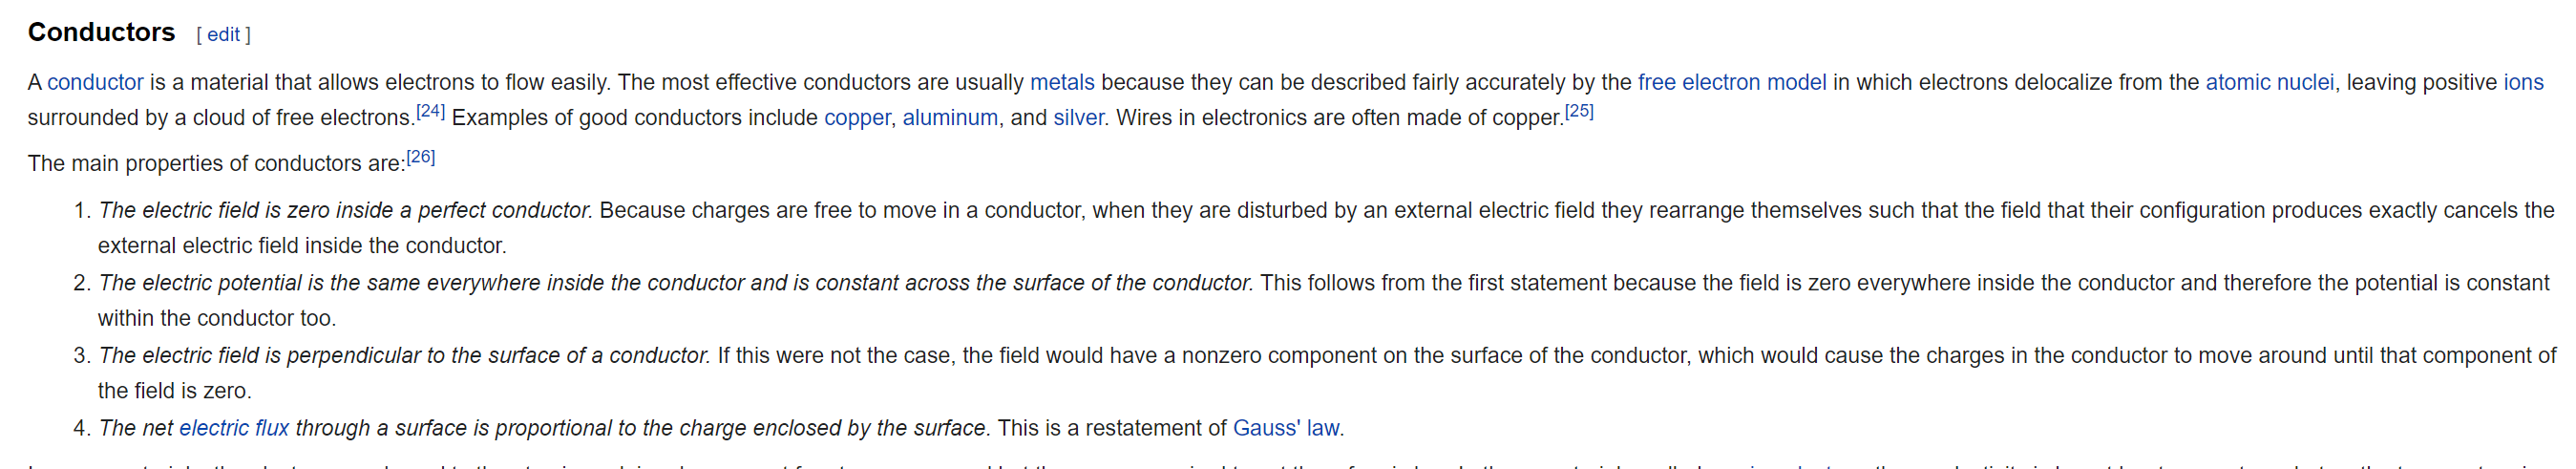
\includegraphics[width=\textwidth]{figures/conductors.png}
    \caption{\textcolor{red}{This may be nice to include in this discussion}}
\end{figure}

\colin{In all of these examples it seems to look like we get that the media have constant permativity, capacitiance, permeability, or inductance. This is really just an artifact of choice. The non-constant and even potentially anisotropic behavior of a media is definitely interesting, but it is all geometric and literally comes from the Riemannian metric. Something should probably be said about this in a more exact way.}

\subsection{3-Dimensional Cavity}

\colin{Giaquinta pg 599 starts intersection}

Let $M$ be the 3-dimensional manifold with boundary given by taking a ball of radius 2 centered at the origin and removing a ball of radius 1 centered at the origin. We refer to $M$ as a spherical cavity.
\begin{figure}[H]
	\centering
	%\def\svgwidth{\columnwidth}
	%\resizebox{.35\columnwidth}{!}{\input{figures/cavity.pdf_tex}}
	\includesvg[width=.35\textwidth]{svg/cavity.svg}
\end{figure}
This space and its boundary has the following absolute and relative homology given by the long exact sequence:
% \begin{align*}
%     H_0(M) &\cong \R &&& H_0(M,\partial M) &\cong 0 &&& H_0(\partial M) &\cong \R^2\\
%     H_1(M) &\cong 0 &&& H_1(M,\partial M) &\cong \R &&& H_1(\partial M) &\cong 0\\
%     H_2(M) &\cong \R &&& H_2(M,\partial M) &\cong 0 &&& H_2(\partial M) &\cong \R^2\\
%     H_3(M) &\cong 0 &&& H_3(M,\partial M) &\cong \R &&& H_3(\partial M) &\cong 0.
% \end{align*}

\[
% https://tikzcd.yichuanshen.de/#N4Igdg9gJgpgziAXAbVABwnAlgFyxMJZAJgBoBGAXVJADcBDAGwFcYkQAJAfWIAoBZAJQACADqiAxgQDmY0QFt6OABYAjVcABKAXxDbS6TLnyEUAZgrU6TVu259+pcWnoAnPE2FDxUsLIAMegYgGNh4BETkljQMLGyInDy8zm4ejF6CPjJyiirqWtoAesRBhmEmRGT+VrG2CdxmApmS2YH6ZcYR5qTVMTbxiY2OKe5Ynt4tfjlKaho6pSFG4abIUb3WcXZcjSNpGVlTbcGhnSv+PTX97Ecdy0TnVH2bCT5QEDgI7YvlXcgALBcnnUQK93p9jksKigAY8NsDQR8Fic7ihzsRLs8QZI3oivsioatSOigQNuORkqIXKNxs1fLJxLlZgUkZDfmRiXDSVxyRM6cIbt9TkQLBzalyeU5KakxuledkGTN8vM8ayVgDRVcXtiwSyfmdSGYMfDtbiIXrIgajVz-BSqXs5VMFXk5kUSirzSgyIaSVsbQ76QpFS7dULut7Ob6BJK7TL9pMAiGUf9LT6Em0rDAoNJ4ERQAAzVwQeRIABsNBwECQAFYvgWi9Xy5XEBYI1r8Dh6IUAFQLOvF5uNpAA1tYgBWjO7vcL-eHFaQAA5U1i8IxYMBdjLdLXp0gAOyDxBkEfiFdrjdMLfBPtIKIgOeIACcS5PWFXMHXUupjEv+Z3iHI5x3k25C3mK7Avm+H4xheU71v+VYHuQZbHqIp7vue36wf25CLkBN5PihaFQdKMHbnB5Atve5DDmBWpERhP4gNeh4HoBtFYu2nY9mR2G3lRR7seInGTjxN7IVR+4ocJ3FXn+gFUc+ojjjMImyeRR5US2glKROMm-uRklUbh2nKSoImUNoQA
\begin{tikzcd}
0 \arrow[r]                          & H_3(\partial M)\cong 0 \arrow[r, "\iota^*"]            & H_3(M)\cong 0 \arrow[r, "\jmath^*"]           & {H_3(M,\partial M)\cong \mathbb{R}} \arrow[r, "\tilde{\partial}"] & \cdots \\
\cdots \arrow[r, "\tilde{\partial}"] & H_2(\partial M)\cong \mathbb{R}^2 \arrow[r, "\iota^*"] & H_2(M) \cong \mathbb{R} \arrow[r, "\jmath^*"] & {H_2(M,\partial M)\cong 0} \arrow[r, "\tilde{\partial}"]          & \cdots \\
\cdots \arrow[r, "\tilde{\partial}"] & H_1(\partial M)\cong 0 \arrow[r, "\iota^*"]   & H_1(M)\cong 0 \arrow[r, "\jmath^*"]           & {H_1(M,\partial M)\cong \mathbb{R}} \arrow[r, "\tilde{\partial}"] & \cdots \\
\cdots \arrow[r, "\tilde{\partial}"] & H_0(\partial M)\cong \mathbb{R}^2 \arrow[r, "\iota^*"] & H_0(M)\cong \mathbb{R} \arrow[r, "\jmath^*"]  & {H_0(M,\partial M)\cong 0} \arrow[r, "\tilde{\partial}"]          & 0     
\end{tikzcd}
\]
\colin{These short exact sequences are dual}
\begin{figure}
    \centering
    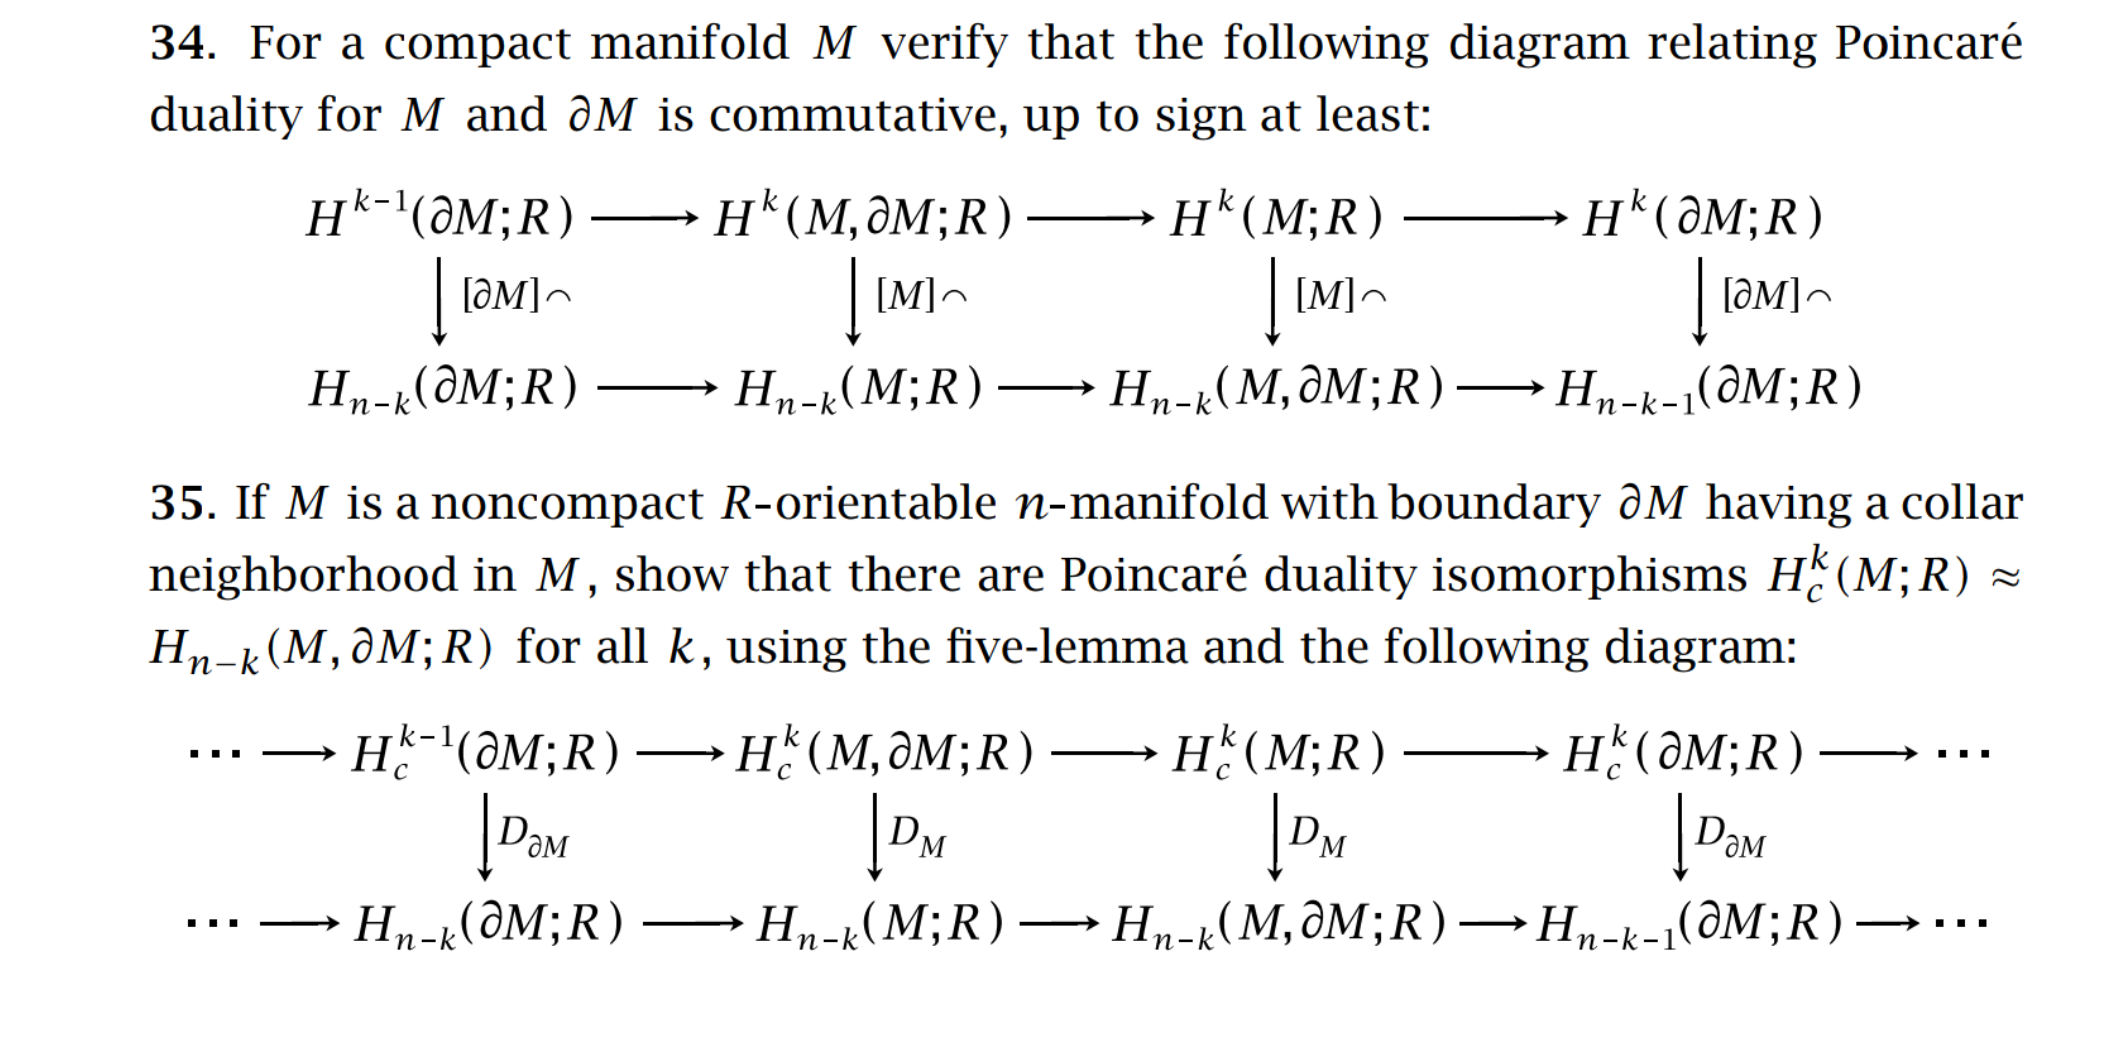
\includegraphics[width=\textwidth]{figures/cap_fundamental_class.png}
    \caption{\textcolor{red}{This will be really useful. Cap with the fundamental class is also a really good way of looking at poincare duality. Is that not just the pseudoscalar dual?? Also, it will be interesting to align the absolute cohomology with $\grad \wedge$ and the relative cohomology with $\grad \cdot$.}}
\end{figure}
We can extract the following short exact sequences from this long exact sequence
\[
% https://tikzcd.yichuanshen.de/#N4Igdg9gJgpgziAXAbVABwnAlgFyxMJZARgBoAGAXVJADcBDAGwFcYkQAJAfQGYAKALKkAOsLT0ATniYACAQEpRAYwIBzGaIC29HAAsARvuAAlAL4hTpdJlz5CKchWp0mrduQtWQGbHgJEAJicaBhY2RE4uAL5RcSksWQVlNQ1hbT1DE1MAPQDPa187Ih5glzD2bmik4RUwdS0dAyMzfO8bP3tkABZS0LcIj1NnGChVeCJQADMJCE0kMhAcCCRySymZucRHReXEILL+kFE8RlhgWMlpRnM1kGnZpH2lpBKD8KPhfBx6bIAqVvum1ez0QPTe7FEACt0ro-hZKKYgA
\begin{tikzcd}
0 \arrow[r] & {H_3(M,\partial M)\cong \mathbb{R}} \arrow[r, "\tilde{\partial}"] & H_2(\partial M)\cong \mathbb{R}^2 \arrow[r, "\iota^*"] & H_2(M)\cong \mathbb{R} \arrow[r, "\jmath^*"] & 0
\end{tikzcd}
\]
\[
% https://tikzcd.yichuanshen.de/#N4Igdg9gJgpgziAXAbVABwnAlgFyxMJZARgBoAGAXVJADcBDAGwFcYkQAJAfWIAoBZUgB0haegCc8TAAT8AlCIDGBAObSRAW3o4AFgCM9wAEoBfECdLpMufIRTkK1Ok1bty5yyAzY8BIgCZHGgYWNkROLnJeETFJLBl5JVV1IS1dA2MTAD1-DysfWyIAZiDnUPZuKMShZTA1TW19Q1M8r2tfO2QAFlKQ13D3EycYKBV4IlAAM3EIDSQyEBwIJHILKZm5xAdF5cRAsv6QETxGWGAYiSlGMzWQadmkfaWkEoOwo6F8HHosgCpW+6bV7PRA9N7sEQAKzSOj+5koJiAA
\begin{tikzcd}
0 \arrow[r] & {H_1(M,\partial M)\cong \mathbb{R}} \arrow[r, "\tilde{\partial}"] & H_0(\partial M)\cong \mathbb{R}^2 \arrow[r, "\iota^*"] & H_0(M)\cong \mathbb{R} \arrow[r, "\jmath^*"] & 0
\end{tikzcd}.
\]

\subsection{Gradients}
If we take the second sequence, we note that since this is short and exact,
\begin{equation}
    H_0(M) \cong H_0(\partial M) ~ / ~ \im \tilde{\partial}
\end{equation}
Noting that $H_0(M)\cong \monogenics^0_N(M)$ we realize that $H_0(M)$ consists solely of classes of constant functions parameterized by $\R$. The same argument shows that since $\partial M$ is closed and is two connected components, $H_0(\partial M)$ is consists of pairs of constant functions each defined on the two connected components. \textcolor{red}{It must be that $\im \tilde{\partial}\cong \ker \iota^*$ represents the diagonal, i.e., for $(c_1,c_2)\in H_0(\partial M)$ we have $\iota^*(c_1,c_2) = c_2-c_1$ so that the pairs of identical constant functions $(c,c)$ are in the kernel and so that the quotient makes sense. But any such constant times this map yields the same kernel, i.e. $\lambda(c_2-c_1)$.} Recall that $H_1(M,\partial M)\cong \monogenics^1_D(M)$ and note that since $H_1(M)\cong 0$ all periods of fields in $\monogenics^1_D(M)$ vanish and by \cite[Theorem 6, pg. 598]{giaquinta_cartesian_1998-1}, it must be that any $\blade{E}\in H_1(M,\partial M)$ is of the form $\blade{E} = \grad \wedge \phi$ for $\phi \in \G^0(M)$. In particular, in order for $\blade{E}$ to be nontrivial, $\phi\vert_{\partial M} \in H_0(\partial M)$ must not be in the kernel of $\iota^*$ so $\phi\vert_{\partial M_1}=\lambda c_1$ and $\phi\vert_{\partial M_2}=\lambda c_2$ with $c_1 \neq c_2$ and so the difference between the boundary values is $\lambda(c_2-c_1)$ and still lies in the kernel of $\iota^*$. Any $\phi \in \G^0(M)$ satisfying these boundary constraints works (including where $c_1=c_2$), but there is a unique representative satisfying $\Delta \phi = 0$ (see \cref{eq:dirichlet_problem} and \cite[Theorem 3.4.6]{schwarz_hodge_1995}) which is the minimal energy $\phi$ or the minimal mass current \colin{I also should explain this}. This is exactly the the scalar potential! One can see that if $c_1=c_2=c$, then this forces $\phi=\lambda c$ on all of $M$ whereas if $c_1\neq c_2$, $\phi(r)=c_1+\lambda (c_2-c_1)(r-1)$ satisfies $\Delta \phi = 0$ since it is a field dependent linear in the radial variable $r$. \textcolor{red}{It even seems that $\iota^*$ appears in the ``slope" term. The ratio $(c_2-c_1)/(\grad \phi) = \lambda$ is the permittivity (or polarization or capacitance) of the cavity itself.} 
\colin{There are some secret backward arrows that are probably showing up here for the relative cohomology story. For example, the $E\in H_1(M,\partial M)$ is of the form $E=\grad \wedge \phi$ is backwards from $ \tilde{\partial} \colon H_1(M,\partial M) \to H_0(\partial M)$. Can we take the Poincare--Lefschetz dual of the whole LES? I believe it will give you what Hatcher has on page 200.}
\colin{Probably mention the fact that $curl\circ grad = 0$ is always true but we are extracting more. All of this really has to do with the solvability of finding a potential for any electric field.}

\subsubsection{Divergences}
\textcolor{red}{The other sequence should tell us about when scalar fields are divergences? This should relate to the charge density! It is that grad div = 0?}
If we look at the first short exact sequence
\[
% https://tikzcd.yichuanshen.de/#N4Igdg9gJgpgziAXAbVABwnAlgFyxMJZARgBoAGAXVJADcBDAGwFcYkQAJAfQGYAKALKkAOsLT0ATniYACAQEpRAYwIBzGaIC29HAAsARvuAAlAL4hTpdJlz5CKchWp0mrduQtWQGbHgJEAJicaBhY2RE4uAL5RcSksWQVlNQ1hbT1DE1MAPQDPa187Ih5glzD2bmik4RUwdS0dAyMzfO8bP3tkABZS0LcIj1NnGChVeCJQADMJCE0kMhAcCCRySymZucRHReXEILL+kFE8RlhgWMlpRnM1kGnZpH2lpBKD8KPhfBx6bIAqVvum1ez0QPTe7FEACt0ro-hZKKYgA
\begin{tikzcd}
0 \arrow[r] & {H_3(M,\partial M)\cong \mathbb{R}} \arrow[r, "\tilde{\partial}"] & H_2(\partial M)\cong \mathbb{R}^2 \arrow[r, "\iota^*"] & H_2(M)\cong \mathbb{R} \arrow[r, "\jmath^*"] & 0
\end{tikzcd}
\]
we arrive at 
\begin{equation}
    H_2(M) \cong H_2(\partial M) ~/~ \im \tilde{\partial}
\end{equation}
and again we can replace $\im \tilde{\partial}$ with the equivalent $\ker \iota^*$. The analysis of this short exact sequence will feel extremely similar to the previous one. Really it is due to the fact that the connected components of the boundary of $M$ are spheres, so $H_0(\partial M)$ and $H_2(\partial M)$ feel similar. In particular, the map $\iota^*$ includes the homological chains from $H_2(\partial M)$ into $H_2(M)$ and kills off by the diagonal. In particular, we can write a class $(c_1,c_2) \in H_2(\partial M)$ and let $\iota^*(c_1,c_2)=\lambda (c_2-c_1)$; the inclusion of $\lambda$ since this does not change $\ker \iota^*$. One could also consider $c_2+c_1$ and the inclusion would kill of chains oriented in opposite directions, which is perhaps more sensible.

We realize $H_2(M)\cong H^1(M,\partial M)$ by Poincar\'e--Lefschetz and moreover that $H^1(M,\partial M)\cong \monogenics^1_D(M)$ by the Hodge isomorphism. So, in reality, our analysis here is only different in $H_2(\partial M)$, but since $\partial M$ is closed, $H_2(\partial M)\cong H_0(\partial M)$, so the content of this short exact sequence seems to be the same as the other. We can still draw a new conclusion.

Thinking of $H_2(\partial M)$ as being flux through the boundary as opposed to thinking of $H_0(\partial M)$ as a scalar field, we have the relationship through Stokes' theorem. Let $\blade{E}$ be a vector field then
\begin{equation}
    \int_M (\grad \wedge \blade{E}^\perp)\contract dX_3 = \int_M \grad \contract \blade{E} \mu= \int_{\partial M} (\blade{E}^\perp,\pseudoscalar_\partial) \mu_\partial 
\end{equation}
which first of all lets us see that the exterior derivative of a bivector in 3-dimensions is the divergence just and the dual is the interior derivative of a vector field. If $\blade{E}^\perp \in \ker \grad \wedge$, then $\blade{E}^\perp$ must also have no tangential components along the boundary, i.e., no flux. In particular, if $\blade{E}^\perp \in \monogenics^2_D(M)$. In fact, since $H_3(M)$ vanishes, all periods of $\rho \in H^3(M)$ vanish, and since there is only the trivial class of $M$, 
\begin{equation}
    \int_M \rho \contract dX_3 = 0.
\end{equation}
But, we see that this means $\rho = \grad \wedge \blade{E}^\perp$ for some $\blade{E}^\perp$ and hence any trivector $\rho$ is the divergence of some bivector field $\blade{E}^\perp$. Of course, we could have dualized using $\perp$ all along and note that any $\rho_0 \in H^0(M,\partial M)$ is of the form $\rho_0 = \grad \contract \blade{E}$ for a vector field $\blade{E}$.
\colin{Probably mention the fact that $div\circ curl = 0$ is always true but we are extracting more. All of this really has to do with the solvability of finding an electric field from a charge distribution $\rho$} 


\colin{It is probably going to be useful to use this LES to probe deeper into where these things come from and relate them to boundary value problems. E.g., charging the boundary spheres with opposite charge or something. This deserves more of a discussion.}\colin{It is probably worth explaining exactly what these classes are and how you can arrive at some of these conclusions via duality and stuff. It also becomes quite clear in the table above.}



\subsubsection{Intersection Product}

\colin{The intersection product tells us which currents provide the same (albeit dual) measurements! For example, you measure electric field (and therefore charge) by using an $H_2(M)$ or an $H_1(M,\partial M)$ class. To measure (or even have) free current, you need an $H_1(M)$ or $H_2(M,\partial M)$ class. If two currents intersect, then they're capable of measuring the same properties of the same type of field. These examples show that. I also think this is some of the purpose of using homology. The intersection in homology gives us integer valued results and I don't know if there is an example of this in cohomology.}
The intersection product on currents is given by the map
\begin{equation}
i\colon H_k(M,\partial M) \times H_{n-k}(M) \to \Z.
\end{equation}
\colin{Giaquinta shows this maps into $\Z$} To interpret this mapping concretely, let us take $S\in H_1(M,\partial M)$ and $T\in H_2(M)$ as in the figure below.
\begin{figure}[H]
	\centering
	%\def\svgwidth{\columnwidth}
	%\resizebox{.35\columnwidth}{!}{\input{figures/cavity_homology.pdf_tex}}
	\includesvg[width=.35\textwidth]{svg/cavity_homology.svg}
    \caption{The second homology class $T$ and first relative homology class $S$.}
\end{figure}
It is quite clear that we should see $i(S,T)=1$. \colin{I can do this explicitly in coordinates.}

There are a few possible interpretations of this intersection granted to us by Lefschetz duality and the Hodge isomorphisms 
\begin{align*}
    H_{n-k}(M) &\mycong{P} H^k(M,\partial M) \mycong{H} \harmonic^k_D(M) \mycong{$\star$} \harmonic^{n-k}_N(M)\\
    H_k(M,\partial M) &\mycong{P} H^{n-k}(M) \mycong{H} \harmonic^{n-k}_N(M) \mycong{$\star$} \harmonic^{k}_D(M),
\end{align*}\colin{I should also include the dual chain with $\grad \cdot$ in here.}
where P denotes the Poincar\'e-Lefschetz duality isomorphism, H denotes the Hodge isomorphism, and $\star$ denotes the Hodge star isomorphism.

\subsubsection{Intersection as flux}
If we again consider the intersection map on $H_1(M,\partial M) \times H_{2}(M)$, we can replace the first factor with $\harmonic^1_D(M)$ and so there is a harmonic vector field $\blade{E}$ corresponding to the relative 1-current $S$ by virtue of
\begin{align*}
i(S,T) = T[\blade{E}^\perp] = \int_T(\blade{I}_T,\blade{E}^\perp)= \int_T (\blade{\nu},\blade{E}) \mu_T = 1. && \textrm{(Flux)}
\end{align*}
\colin{$\perp$ here is acting as the Hodge star so you can see what the Neumann form is as well.}
In other words, intersections can be computed by fluxes.\colin{In fact, this is just one type of flux one may call "capacitive". The "inductive" flux would come in the torus example.} In order for this to be a homological invariant, it must be that the flux of $\blade{E}$ through any 2-cycle is invariant and since $H_1(M)$ vanishes, we see that $\blade{E}$ is a gradient field $\blade{E}=\grad \wedge \phi$. But, this is in fact given to us through the LES of relative homology. Note that for this case, we have a short exact sequence 
\[
H_1(M) \cong 0 \xrightarrow{~\jmath_*~} H_1(M,\partial M)\cong \mathbb{R} \xrightarrow{~\tilde{\partial}~} H_0(\partial M) \cong \mathbb{R}^2 \xrightarrow{~\iota_*~} H_0(M)\cong \mathbb{R} \xrightarrow{~\jmath_*~} H_0(M, \partial M)\cong 0.
\]
\[
\begin{tikzcd}
H_1(M)\cong 0 \arrow[rr, "\jmath_*"] &  & {H_1(M,\partial M)\cong \mathbb{R}} \arrow[rr, "\tilde{\partial}"] &  & H_0(\partial M) \cong \mathbb{R}^2 \arrow[rr, "\iota_*"] &  & H_0(M)\cong \mathbb{R} \arrow[rr, "\jmath_*"] &  & {H_0(M,\partial M)\cong 0}
\end{tikzcd}
\]
Hence $H_0(M)\cong H_0(\partial M)~/~ \tilde{\partial}(H_1(M,\partial M))$. Thinking dually, $H_0(M)\cong\harmonic^0_D(M)$ and $H_0(\partial M)\cong \harmonic^2(\partial M)$; since $\partial M$ is closed we need not account for boundary conditions. \colin{Okay, I'm not sure how this sequence gives some kind of intuitive answer but I'll explain the intuitive thing now. It is probably worth thinking about what we are quotienting by in terms of $\grad \wedge$.} The topology is giving us the physical insight that we can consider a scalar field $\phi \colon \partial M \to \R$ with $\phi=1$ on the inner shell and $\phi=0$ on the outer. Extend $\phi$ to $M$ by smoothly by radially interpolating, then $\grad \wedge \phi \in H^1_D(M)$. 

We can think of $\blade{E}$ as a harmonic mollification of the current (relative 1-cycle) $S$ to be distributed in such a way that the intersection is preserved. In particular, if we chose unit speed rays emanating from the origin in all possible directions, the tangent vectors would give us this field.

\subsubsection{Intersection as work}
We have the second factor of $H_1(M,\partial M) \times H_{2}(M)$ to consider isomorphisms of. For this case, take $H_2(M)\cong \harmonic^1_D(M)$. Then we have, again, a Dirichlet harmonic vector field $\blade{E}$ corresponding to $T$ satisfying
\begin{align*}
i(S,T) = S[\blade{E}] = \int_S (I_S,\blade{E}) \mu_S = 1 && \textrm{(Work)}.
\end{align*}
Here we see that we can think of $\blade{E}$ as being a harmonic mollification of the normal field to $T$ distributed in $M$. One could think of this as taking normal fields to all the spheres increasing from radius 1 to 2.

So there is a natural duality between flux and work familiar to us from a multivariate calculus course.


\subsection{Solid Torus}
\colin{I think it may be worth thinking about this more as two linked circles, in a way. I know it isn't literally two linked circles, but I think that is closer to an inductor}
Let $M$ be the 3-dimensional manifold with boundary given by taking a solid torus with inner radius 1 and outer radius 2 centered at the origin. We refer to $M$ as the solid torus.
\begin{figure}[H]
	\centering
	%\def\svgwidth{\columnwidth}
	%\resizebox{.35\columnwidth}{!}{\input{figures/torus.pdf_tex}}
	\includesvg[width=.35\textwidth]{svg/torus.svg}
\end{figure}

This space and its boundary has the following absolute and relative homology (noting that the boundary has no relative homology) \colin{Am I missing an SES passing through the fundamental class $H_3(M,\partial M)$??}\colin{Could get this homology using Kunneth formula? Also homotopy equivalent to $S^1$}:
% \begin{align*}
%     H_0(M) &\cong \R &&& H_0(M,\partial M) &\cong 0 &&& H_0(\partial M) &\cong \R\\
%     H_1(M) &\cong \R &&& H_1(M,\partial M) &\cong 0 &&& H_1(\partial M) &\cong \R^2\\
%     H_2(M) &\cong 0 &&& H_2(M,\partial M) &\cong \R &&& H_2(\partial M) &\cong \R\\
%     H_3(M) &\cong 0 &&& H_3(M,\partial M) &\cong 0 &&& H_3(\partial M) &\cong 0.
% \end{align*}
\[
% https://tikzcd.yichuanshen.de/#N4Igdg9gJgpgziAXAbVABwnAlgFyxMJZAJgBoBGAXVJADcBDAGwFcYkQAJAfWIAoBZAJQACADqiAxgQDmwgAwgAvqXSZc+QigDMFanSat23Pv1Li09AE54mwoeKlhZ4gLb0cACwBGX4ACVFJRUQDGw8AiJyXRoGFjZETh5ecysbRjtBBxkxUTdPH39A5VUwjSIyOT1YwwTuLQFMyWyFYpC1cM1kHUqYg3jE+tMU6yxbeyaneSCS9QiUKJ79OKMueuG0jKzJluDQ2c65UkXq-p2ZjqJDql7lhIcoCBwEVr2LlAAWI6q+9nvH5927TKH2iSxqID+T2mbVKc2Qh2I31uEMkDyhLyBcKiiJu4O45GSogsIzGjUczly7m8vgCAD1iNDXsCSKQcWD+viGlsKXlqYVGZjOjo2ScVgShkTUqN0uNyVMMbDOp8RT87qj-gLFZdSFokeDIQDzsyorrcRyuHJCcSNrLsq4qQUApr9uUdXrzZbbZN7fkaUVAVrtG6zStPWZJSSZWTms63shPqb2ewWnoYFBpPAiKAAGaWCAuJAANhoOAgSAArK1c-mKyWy4gdEm1fgcPRaQAqaHVgsNutIT5NlEAK15Ha7eZ7A9LSAAHCG1XhGLBgOtpf6cxOkAB2PuIMiD8SL5erpjrkDdpBREDTxAATnnKKPMBXEbSZ4viHIh2v9fIV9FC5YEuz4now76bp+5a7uQxYHqIT4vtaa7jjWn5zj+l73nBCGgeBqHkI2N7kAOAGPkBx6vshVYQfuN7fqR4gtm2nbUfhV5EfuDGiExY6sT2MHQTucE8SxwQft+REPuII5UrxYkQeQtG-o2XEyZ4ckbvhQlEehqmjixlCKEAA
\begin{tikzcd}
0 \arrow[r]                          & H_3(\partial M)\cong 0 \arrow[r, "\iota^*"]            & H_3(M)\cong 0 \arrow[r, "\jmath^*"]          & {H_3(M,\partial M)\cong \R} \arrow[r, "\tilde{\partial}"]          & \cdots \\
\cdots \arrow[r, "\tilde{\partial}"] & H_2(\partial M)\cong \mathbb{R} \arrow[r, "\iota^*"]   & H_2(M) \cong 0 \arrow[r, "\jmath^*"]         & {H_2(M,\partial M)\cong \mathbb{R}} \arrow[r, "\tilde{\partial}"] & \cdots \\
\cdots \arrow[r, "\tilde{\partial}"] & H_1(\partial M)\cong \mathbb{R}^2 \arrow[r, "\iota^*"] & H_1(M)\cong \mathbb{R} \arrow[r, "\jmath^*"] & {H_1(M,\partial M)\cong 0} \arrow[r, "\tilde{\partial}"]          & \cdots \\
\cdots \arrow[r, "\tilde{\partial}"] & H_0(\partial M)\cong \mathbb{R} \arrow[r, "\iota^*"]   & H_0(M)\cong \mathbb{R} \arrow[r, "\jmath^*"] & {H_0(M,\partial M)\cong 0} \arrow[r, "\tilde{\partial}"]          & 0     
\end{tikzcd}
\]
\colin{It is probably worth explaining exactly what these classes are and how you can arrive at some of these conclusions via duality and stuff. It also becomes quite clear in the table above.}
\[
\begin{tikzcd}
\cdots \arrow[r] & H_k(\partial M) \arrow[r, "\iota_*"] & H_k(M) \arrow[r, "\jmath_*"] & {H_k(M,\partial M)} \arrow[r, "\tilde{\partial}"] & H_{k-1}(\partial M) \arrow[r] & \cdots
\end{tikzcd}
\]
There are two short exact sequences in the above long exact sequence. First is 
\[
% https://tikzcd.yichuanshen.de/#N4Igdg9gJgpgziAXAbVABwnAlgFyxMJZABgBpiBdUkANwEMAbAVxiRAAkB9AJgAoBZAJQAdYQGMCAcwAExEAF9S6TLnyEUARnJVajFmy59+pUWjoAnPI2lDREsDNEBbOjgAWAIw-AASvIVKIBjYeARE3NrU9MysiBycGrymFlYMNiLiUtLOrp7efgB63AHKIWpEAMyRujEGCQIZ9o7CLu5evv6KpaphKAAs1dH6cVyJxsmWWNZC2ZkOcvI6MFCS8ESgAGbmEE5IZCA4EEgaXSBbO8fUh0gRNcMgongMsMATqZ2B57uIt9eIVXdYg9hPgcHQCgAqEpnbbfAF-AaAtiiABWrTckIUFHkQA
\begin{tikzcd}
0 \arrow[r] & {H_2(M,\partial M)\cong \mathbb{R}} \arrow[r, "\tilde{\partial}"] & H_1(\partial M)\cong \mathbb{R}^2 \arrow[r, "\iota^*"] & H_1(M)\cong \mathbb{R} \arrow[r] & {0}
\end{tikzcd}
\]
and the second
\[
\begin{tikzcd}
0 \arrow[r] & {H_3(M,\partial M)\cong \mathbb{R}} \arrow[r, "\tilde{\partial}"] & H_2(\partial M)\cong \mathbb{R} \arrow[r, "\iota^*"] & {0}
\end{tikzcd}
\]
In the first sequence we see that
\[
H_1(M) \cong H_1(\partial M) ~/~ \im \tilde{\partial}
\]
and we can again note that $\im \tilde{\partial} = \ker \iota^*$. Using the same isomorphisms as the cavity (just with different grades now), we have $H_1(M)\cong \monogenics^1_N(M)$ and $H_2(M,\partial M) \cong M^1_N(M)$. Now, $H_2(M)\cong 0$ leaving no second absolute homology classes and so it must be that there exists $\blade{j} \in M^1_N(M)$ that is the curl $\grad \cdot B =\blade{j}$ for $B\in \G^2(M)$. Moreover, there exists a unique such a $B$ where $\Delta B=0$ which implies that the divergence $\grad \wedge B = 0$. This $B$ is exactly the magnetic bivector field and $\blade{j}$ is the current vector field. Inherently, our choices for the grades of $\blade{j}$ and $B$ were artifacts of intuition from knowledge of the relativistic theory (which we will approach soon). Applying $\perp$ to all of the logic above, we see Ampere's law $\blade{j}^\perp = \grad \wedge B^\perp$ and Gauss's law $\grad \cdot B^\perp = 0$ via the vector divergence. \colin{Ampere's law also show us that current chains must have no boundary. The example of an infinite line current is really a closed loop on $S^3$.}

The short exact sequence tells us more. Indeed, it really says that our $\blade{j}\in H_1(M) \cong \monogenics^1_N(M)$ arises via an absolute homology class on the boundary $\blade{j}\vert_{\partial M} \in H_1(\partial M)$. There are two such classes and we write $(c_1,c_2)\in H_1(\partial M)$ as a pair of such classes where the first component $c_1$ represents the solenoidal (or toroidal) class tangent to the boundary $\partial S$ and the second component $c_2$ the circulating class we achieve by homotoping $T$ to $\partial M$. If we prescribe a homology class for $\blade{j}\vert_{\partial M} = (c_1,0)$, then the corresponding $B$ must be solely in the absolute homology class of $M$, i.e., $B\in H_1(M) \cong \monogenics^2_D(M)$ which when homotoped to the boundary represents the circulating homology class $B\vert_{\partial M}(0,c_2)\in H_1(\partial M)$ and is Poincar\'e--Lefschetz dual to the class $B\in H_2(M,\partial M)$. \textcolor{red}{The ratio $c_2/c_1$ we get from this process is the permeability (or magnetization or inductance) of the solid torus itself.}


In the second SES
\[
\begin{tikzcd}
0 \arrow[r] & {H_3(M,\partial M)\cong \mathbb{R}} \arrow[r, "\tilde{\partial}"] & H_2(\partial M)\cong \mathbb{R} \arrow[r, "\iota^*"] & {0}
\end{tikzcd}
\]
we see that $H_2(\partial M) \cong H_3(M,\partial M)$ and moreover the map $\tilde{\partial}$ is an isomorphism. \colin{I have no clue what this means as far as fields. I honestly almost forgot the fundamental class in this example.}

\subsubsection{Intersection}

The intersection product on currents is given by the map
\begin{equation}
i\colon H_k(M,\partial M) \times H_{n-k}(M) \to \Z.
\end{equation}
\colin{Giaquinta shows this maps into $\Z$} To interpret this mapping concretely, let us take $S\in H_1(M,\partial M)$ and $T\in H_2(M)$ as in the figure below.
\begin{figure}[H]
	\centering
	%\def\svgwidth{\columnwidth}
	%\resizebox{.35\columnwidth}{!}{\input{figures/cavity_homology.pdf_tex}}
	\includesvg[width=.35\textwidth]{svg/torus_homology.svg}
    \caption{The first homology class $T$ and second relative homology class $S$.}
\end{figure}
It is quite clear that we should see $i(S,T)=1$. \colin{I can do this explicitly in coordinates.}

\colin{Okay, I'm not sure how this sequence gives some kind of intuitive answer but I'll explain the intuitive thing now. It is probably worth thinking about what we are quotienting by in terms of $\grad \wedge$.} The topology is giving us the physical insight that we can consider a vector field $\blade{j} \in \G^1(\partial M)$ that is in the same homology class as $\partial S$. This surface current would give rise to a magnetic bivector $\blade{B}$ field tangent to $S$ or with $\blade{B}^\perp=T$. \colin{It is worth thinking about what the other homology class does. It should give a magnetic field that is a Neumann field that looks like a vortex on each $S$}

We can think of $\blade{B}$ as a harmonic mollification of the current (relative 2-cycle) $S$ to be distributed in such a way that the intersection is preserved. \colin{It is like distributing those surfaces of $S$ around the whole solid torus}

\subsubsection{Intersection as flux}
We have the intersection map on $H_2(M,\partial M) \times H_{1}(M)$ to consider isomorphisms of. For this case, take $H_1(M)\cong \monogenics^2_D(M)$. Then we have a Dirichlet monogenic bivector field $\blade{B}\in \monogenics^2_D(M)$ corresponding to $T$ satisfying
\begin{align*}
i(S,T) = S[\blade{B}] = \int_S (\pseudoscalar_S,\blade{B}) \mu_S = \int_S (\normal_S,\blade{B}^\perp) \mu_S  = 1 && \textrm{(Flux)}.
\end{align*}
\colin{This may look a bit different than how I have the integrals over chains. THose really need a pullback in them and that pullback corresponds to taking tangential components}
Here we see that we can think of $\blade{B}$ as being a harmonic mollification of the normal field to $T$ distributed in $M$. If you'd like, $\blade{B}^\perp \in \monogenics^1_N(M)$ is the vector field corresponding to harmonic flow around the interior of the torus.  

\textcolor{red}{So it seems like "minimal mass $k$-currents" have a direct correspondence to two unique monogenic fields of grade $k$ and $n-k$. For instance, the curve (current) $T$ corresponds to a vector field that has $T$ as a flow, but it is distributed evenly inside of $M$. Is there some way of writing this down very explicitly? Giaquinta's existence of minimal mass currents stuff could be really nice.}

\subsubsection{Intersection as work}
If we consider the intersection map on $H_2(M,\partial M) \times H_{1}(M)$, we can replace the first factor with $\monogenics^1_N(M)$ and so there is a monogenic vector field $\blade{B}^\perp\in \monogenics^1_N(M)$ corresponding to the relative 2-current $S$ by virtue of
\begin{align*}
i(S,T) = T[\blade{B}^\perp] = \int_T(\blade{I}_T,\blade{B}^\perp)\mu_T= 1. && \textrm{(Work)}
\end{align*}
\colin{In fact, this is just one type of flux one may call "inductive". } In order for this to be a homological invariant, it must be that the flux of $\blade{B}^\perp$ through any relative 2-cycle is invariant and since $H_2(M)$ vanishes, we see that $\blade{B}$ is a curl field $\blade{B}=\grad \wedge \blade{j}$. But, this is in fact given to us through the LES of relative homology. Note that for this case, we have a short exact sequence 
\colin{I need to redo this sequence}
\[
H_1(M) \cong 0 \xrightarrow{~\jmath_*~} H_1(M,\partial M)\cong \mathbb{R} \xrightarrow{~\tilde{\partial}~} H_0(\partial M) \cong \mathbb{R}^2 \xrightarrow{~\iota_*~} H_0(M)\cong \mathbb{R} \xrightarrow{~\jmath_*~} H_0(M, \partial M)\cong 0.
\]
\[
\begin{tikzcd}
H_1(M)\cong 0 \arrow[rr, "\jmath_*"] &  & {H_1(M,\partial M)\cong \mathbb{R}} \arrow[rr, "\tilde{\partial}"] &  & H_0(\partial M) \cong \mathbb{R}^2 \arrow[rr, "\iota_*"] &  & H_0(M)\cong \mathbb{R} \arrow[rr, "\jmath_*"] &  & {H_0(M,\partial M)\cong 0}
\end{tikzcd}
\]
\colin{I need to rewrite this}
Hence $H_0(M)\cong H_0(\partial M)~/~ \tilde{\partial}(H_1(M,\partial M))$. Thinking dually, $H_0(M)\cong\harmonic^0_D(M)$ and $H_0(\partial M)\cong \harmonic^2(\partial M)$; since $\partial M$ is closed we need not account for boundary conditions. \colin{Okay, I'm not sure how this sequence gives some kind of intuitive answer but I'll explain the intuitive thing now. It is probably worth thinking about what we are quotienting by in terms of $\grad \wedge$.} The topology is giving us the physical insight that we can consider a scalar field $\phi \colon \partial M \to \R$ with $\phi=1$ on the inner shell and $\phi=0$ on the outer. Extend $\phi$ to $M$ by smoothly by radially interpolating, then $\grad \wedge \phi \in H^1_D(M)$. 

We can think of $\blade{E}$ as a harmonic mollification of the current (relative 1-cycle) $S$ to be distributed in such a way that the intersection is preserved. In particular, if we chose unit speed rays emanating from the origin in all possible directions, the tangent vectors would give us this field.



\colin{I think this is really interesting stuff that could come in with plasmas too \url{https://cseweb.ucsd.edu/~alchern/notes/GeometricFluidDynamics/} I'm thinking of it because the pictures we're making here seem to be the same as this.}

\subsection{Periodic Cavity}

\colin{It seems like Kotuiga in his thesis \cite{kotiuga_hodge_nodate} basically talks about how these next parts here could be interesting but doesn't do it and I haven't found anyone else who has. Also he has an excellent more modern book we need to cite \cite{gross_electromagnetic_2004}}
Let $N^3$ be the cavity from before and let us consider the 4-manifold $M=N^3 \times S^1$. Note that this manifold admits global coordinates $(x,y,z,t)$ where $t$ is the angular coordinate on $S^1$. Moreover, $M$ is metrizable with a semi-Riemannian metric of signature $(+,+,+,-)$. In other words, $M$ is a valid spacetime. 
\colin{I think on a general spacetime foliated manifold, the Dirac operator restricted to the spatial leaves of the foliation is still elliptic. Can this be leveraged into something? Something like a time varying Hodge theory?}

We then have that 
\begin{equation}
    \partial M = \partial N^3 \times S^1
\end{equation}
since $\partial S^1 = \emptyset$. The homology for $S^1$ is then $H_0(S^1)\cong \R$, $H_1(S^1)\cong 0$, and for $k\geq 2$, $H_k(S^1)\cong 0$. We can now use the K\"unneth theorem to see that
\begin{equation}
    \bigoplus_{i+j=k} H_i(N^3)\otimes H_j(S^1) \cong H_k(M).
\end{equation}
So we get
\begin{align*}
    H_0(M) &\cong \underbrace{\R \otimes \R}_{H_0(N^3)\otimes H_0(S^1)} \cong \R\\
    H_1(M) &\cong \underbrace{(\R \otimes \R)}_{H_0(N^3)\otimes H_1(S^1)} \oplus \underbrace{(0 \otimes \R)}_{H_1(N^3)\otimes H_0(S^1)} \cong \R\\
    H_2(M) &\cong \underbrace{(\R \otimes 0)}_{H_0(N^3)\otimes H_2(S^1)} \oplus \underbrace{(0 \otimes \R)}_{H_1(N^3)\otimes H_1(S^1)} \oplus \underbrace{(\R \otimes \R)}_{H_2(N^3)\otimes H_0(S^1)} \cong \R\\
    H_3(M) &\cong \underbrace{(\R \otimes 0)}_{H_0(N^3)\otimes H_3(S^1)} \oplus \underbrace{(0 \otimes 0)}_{H_1(N^3)\otimes H_2(S^1)} \oplus \underbrace{(\R \otimes \R)}_{H_2(N^3)\otimes H_1(S^1)} \oplus \underbrace{(0 \otimes \R)}_{H_3(N^3)\otimes H_0(S^1)} \cong \R\\
    H_4(M) &\cong \underbrace{(\R \otimes 0)}_{H_0(N^3)\otimes H_4(S^1)} \oplus \underbrace{(0 \otimes 0)}_{H_1(N^3)\otimes H_3(S^1)} \oplus \underbrace{(\R \otimes 0)}_{H_2(N^3)\otimes H_2(S^1)} \oplus \underbrace{(0 \otimes \R)}_{H_3(N^3)\otimes H_1(S^1)} \oplus \underbrace{(0 \otimes \R)}_{H_4(N^3)\otimes H_0(S^1)} \cong 0
\end{align*}
\colin{In $H_3(M)$ I think this corresponds to Faraday's law (in a vacuum?) somehow. This is also seemingly the only ``interesting'' case in here. The rest all come from scalar functions in some way. Please read this comment with a hefty grain of salt}
and similarly 
\begin{align*}
    H_0(\partial M) &\cong \underbrace{\R^2 \otimes \R}_{H_0(\partial N^3)\otimes H_0(S^1)} \cong \R^2 \\
    H_1(\partial M) &\cong \underbrace{(\R^2 \otimes \R)}_{H_0(\partial N^3)\otimes H_1(S^1)} \oplus \underbrace{(0 \otimes \R)}_{H_1(\partial N^3)\otimes H_0(S^1)} \cong \R^2 \\
    H_2(\partial M) &\cong \underbrace{(\R \otimes 0)}_{H_0(\partial N^3)\otimes H_2(S^1)} \oplus \underbrace{(0 \otimes \R)}_{H_1(\partial N^3)\otimes H_1(S^1)} \oplus \underbrace{(\R^2 \otimes \R)}_{H_2(\partial N^3)\otimes H_0(S^1)} \cong \R^2\\
    H_3(\partial M) &\cong \underbrace{(\R^2 \otimes 0)}_{H_0(\partial N^3)\otimes H_3(S^1)} \oplus \underbrace{(0 \otimes 0)}_{H_1(\partial N^3)\otimes H_2(S^1)} \oplus \underbrace{(\R^2 \otimes \R)}_{H_2(\partial N^3)\otimes H_1(S^1)} \oplus \underbrace{(0 \otimes \R)}_{H_3(\partial N^3)\otimes H_0(S^1)} \cong \R^2\\
    H_4(\partial M) &\cong \underbrace{(\R^2 \otimes 0)}_{H_0(\partial N^3)\otimes H_4(S^1)} \oplus \underbrace{(0 \otimes 0)}_{H_1(\partial N^3)\otimes H_3(S^1)} \oplus \underbrace{(\R^2 \otimes 0)}_{H_2(\partial N^3)\otimes H_2(S^1)} \oplus \underbrace{(0 \otimes \R)}_{H_3(\partial N^3)\otimes H_1(S^1)} \oplus \underbrace{(0 \otimes \R)}_{H_4(\partial N^3)\otimes H_0(S^1)} \cong 0.
\end{align*}
\colin{The Kunneth theorem should also be helping us see WHERE the homology actually comes from. This may be useful. For example, it may let us use the fact that part of the Hodge-Dirac operator is elliptic and we can think of part of the homology as coming from monogenic fields on slices of time (which is true in some circumstances)}

Here is the LES for relative homology where the $H_4(M,\partial M)$ is the fundamental class which we get for free.
\[
\begin{tikzcd}
0 \arrow[r]                          & H_4(\partial M)\cong 0 \arrow[r, "\iota^*"]            & H_4(M)\cong 0 \arrow[r, "\jmath^*"]          & {H_4(M,\partial M)\cong \R} \arrow[r, "\tilde{\partial}"]          & \cdots \\
\cdots \arrow[r, "\tilde{\partial}"]                          & H_3(\partial M)\cong \R^2 \arrow[r, "\iota^*"]            & H_3(M)\cong \R \arrow[r, "\jmath^*"]          & {H_3(M,\partial M)\cong \textcolor{red}{\R}} \arrow[r, "\tilde{\partial}"]          & \cdots \\
\cdots \arrow[r, "\tilde{\partial}"] & H_2(\partial M)\cong \mathbb{R}^2 \arrow[r, "\iota^*"]   & H_2(M) \cong \R \arrow[r, "\jmath^*"]         & {H_2(M,\partial M)\cong \textcolor{red}{\R}} \arrow[r, "\tilde{\partial}"] & \cdots \\
\cdots \arrow[r, "\tilde{\partial}"] & H_1(\partial M)\cong \mathbb{R}^2 \arrow[r, "\iota^*"] & H_1(M)\cong \mathbb{R} \arrow[r, "\jmath^*"] & {H_1(M,\partial M)\cong\textcolor{red}{\R}} \arrow[r, "\tilde{\partial}"]          & \cdots \\
\cdots \arrow[r, "\tilde{\partial}"] & H_0(\partial M)\cong \mathbb{R}^2 \arrow[r, "\iota^*"]   & H_0(M)\cong \mathbb{R} \arrow[r, "\jmath^*"] & {H_0(M,\partial M)\cong \textcolor{red}{0}} \arrow[r, "\tilde{\partial}"]          & 0     
\end{tikzcd}
\]
\colin{We can get these missing factors from PL duality. Also the map $H_2(M)\to H_2(M,\partial M)$ is an isomorphism.}
Looking at the first unknown line of the LES 
\[
\begin{tikzcd}
\cdots \arrow[r, "\tilde{\partial}"]                          & H_3(\partial M)\cong \R^2 \arrow[r, "\iota^*"]            & H_3(M)\cong \R \arrow[r, "\jmath^*"]          & {H_3(M,\partial M)\cong \textcolor{red}{????}} \arrow[r, "\tilde{\partial}"]          & \cdots
\end{tikzcd}
\]
we see that we must know $\im \iota^*$, $\ker \iota^*$, $\im \jmath^*$, and $\ker \jmath^*$ but also $\ker \jmath^* = \im \iota^*$. Note that $H_3(\partial M) \cong H_2(\partial N^3) \otimes H_1(S^1)$ and $\im \iota^*$ just includes these classes into $H_3(M) \cong H_2(N^3)\otimes H_1(S^1)$ in the same way the for the 3-dimensional static cavity. So we have $\iota^*[(c_1,c_2)\otimes (c_3)] = (c_2-c_1)\otimes c_3$. Taking the trivial class $c_3$ yields a DC solution whereas any nontrivial class in $e^{i \omega t} \in H_1(S^1)$ for $\omega \in \R$ yields a periodic potential on the boundary components $(c_1 e^{i\omega t}, c_2 e^{i\omega t})$. \textcolor{red}{Actually we should see coupling between the two $H_2(N^3)$ classes  via the $H_1(S^1)$ class. For example, apply $c_1$ on the inner sphere as an alternating charge via $e^{i\omega t}$ then this yields the class $\left(c_1 e^{i\omega t}, kc_1 e^{i(\omega t-\psi)}\right)$.} \colin{Somehow I think this should capture the lagging behavior of a capacitor. If I apply a periodic potential on the inner sphere, it will take time for the field to permeate to the outer sphere, right? This should probably come alongside the $\lambda$ that showed up in the static case. Also should I really be thinking of charge not voltage?} \colin{Also this argument is completely analogous for the $H_0(\partial M)$ part of the sequence}

If we now look at the 2-dimensional part of the sequence
\[
\begin{tikzcd}
\cdots \arrow[r, "\tilde{\partial}"] & H_2(\partial M)\cong \mathbb{R}^2 \arrow[r, "\iota^*"]   & H_2(M) \cong \R \arrow[r, "\jmath^*"]         & {H_2(M,\partial M)\cong \textcolor{red}{????}} \arrow[r, "\tilde{\partial}"] & \cdots
\end{tikzcd}
\]
we can see that on the boundary we get the single contributor $H_2(\partial M) = H_2(\partial N^3)\otimes H_0(S^1)$. The $H_0(S^1)$ is simply a constant, so we arrive at the static DC solution in the previous case. \colin{I have confidence that this somehow corresponds to the DC level that the cavity can support.} \textcolor{red}{Can this DC level analysis retrieve the $k$ that showed up in the alternating voltage from before??}

\textcolor{red}{We still have that fact that in 4d, $\grad \contract \blade{J}=0$}

\subsubsection{Intersection}

\colin{From before, the intersection product should tell us about measurements! It will be particularly interesting in these cases since there is a lot more we can measure (e.g., AC freq and amplitude, DC level, for both voltage and current etc.) This may get to Michael's thoughts about real physical measurement devices. }
\textcolor{red}{First off, we need to get the relative homology classes and it will be worth trying to have some kind of visual for what these things are. E.g., in there is the $H_2(M)\cong H_2(N^3)\otimes H_0(S^1)$ class which should just look like the $H_2(N^3)$ class $[T]$ at some instant in time. Then we would have the $H_3(M)\cong H_2(N^3)\otimes H_1(S^1)$ class which perhaps looks like the $[T]\times [\omega]$ where $\omega$ is a class on $S^1$. Do these correspond to real world measurement devices? Is the direct product actually the right idea? I think this last one would correspond to the AC voltage frequency measurement.}


\subsection{Periodic Torus}


Let $N^3$ be the solid torus from before and let us consider the 4-manifold $M=N^3 \times S^1$. Note that this manifold admits global coordinates $(x,y,z,t)$ where $t$ is the angular coordinate on $S^1$. Moreover, $M$ is metrizable with a semi-Riemannian metric of signature $(+,+,+,-)$. In other words, $M$ is a valid spacetime. 
\colin{I think on a general spacetime foliated manifold, the Dirac operator restricted to the spatial leaves of the foliation is still elliptic. Can this be leveraged into something? Something like a time varying Hodge theory?}

We then have that 
\begin{equation}
    \partial M = \partial N^3 \times S^1
\end{equation}
since $\partial S^1 = \emptyset$. The homology for $S^1$ is then $H_0(S^1)\cong \R$, $H_1(S^1)\cong 0$, and for $k\geq 2$, $H_k(S^1)\cong 0$. We can now use the K\"unneth theorem to see that
\begin{equation}
    \bigoplus_{i+j=k} H_i(N^3)\otimes H_j(S^1) \cong H_k(M).
\end{equation}
So we get
\begin{align*}
    H_0(M) &\cong \underbrace{\R \otimes \R}_{H_0(N^3)\otimes H_0(S^1)} \cong \R\\
    H_1(M) &\cong \underbrace{(\R \otimes \R)}_{H_0(N^3)\otimes H_1(S^1)} \oplus \underbrace{(\R \otimes \R)}_{H_1(N^3)\otimes H_0(S^1)} \cong \R^2\\
    H_2(M) &\cong \underbrace{(\R \otimes 0)}_{H_0(N^3)\otimes H_2(S^1)} \oplus \underbrace{(\R \otimes \R)}_{H_1(N^3)\otimes H_1(S^1)} \oplus \underbrace{(0 \otimes \R)}_{H_2(N^3)\otimes H_0(S^1)} \cong \R\\
    H_3(M) &\cong \underbrace{(\R \otimes 0)}_{H_0(N^3)\otimes H_3(S^1)} \oplus \underbrace{(\R \otimes 0)}_{H_1(N^3)\otimes H_2(S^1)} \oplus \underbrace{(0 \otimes \R)}_{H_2(N^3)\otimes H_1(S^1)} \oplus \underbrace{(0 \otimes \R)}_{H_3(N^3)\otimes H_0(S^1)} \cong \R\\
    H_4(M) &\cong \underbrace{(\R \otimes 0)}_{H_0(N^3)\otimes H_4(S^1)} \oplus \underbrace{(\R \otimes 0)}_{H_1(N^3)\otimes H_3(S^1)} \oplus \underbrace{(0 \otimes 0)}_{H_2(N^3)\otimes H_2(S^1)} \oplus \underbrace{(0 \otimes \R)}_{H_3(N^3)\otimes H_1(S^1)} \oplus \underbrace{(0 \otimes \R)}_{H_4(N^3)\otimes H_0(S^1)} \cong 0
\end{align*}
\colin{In $H_3(M)$ I think this corresponds to Faraday's law (in a vacuum?) somehow. This is also seemingly the only ``interesting'' case in here. The rest all come from scalar functions in some way. Please read this comment with a hefty grain of salt}
and similarly 
\begin{align*}
    H_0(\partial M) &\cong \underbrace{\R \otimes \R}_{H_0(\partial N^3)\otimes H_0(S^1)} \cong \R \\
    H_1(\partial M) &\cong \underbrace{(\R \otimes \R)}_{H_0(\partial N^3)\otimes H_1(S^1)} \oplus \underbrace{(\R^2 \otimes \R)}_{H_1(\partial N^3)\otimes H_0(S^1)} \cong \R^3 \\
    H_2(\partial M) &\cong \underbrace{(\R \otimes 0)}_{H_0(\partial N^3)\otimes H_2(S^1)} \oplus \underbrace{(\R^2 \otimes \R)}_{H_1(\partial N^3)\otimes H_1(S^1)} \oplus \underbrace{(\R \otimes \R)}_{H_2(\partial N^3)\otimes H_0(S^1)} \cong \R^3\\
    H_3(\partial M) &\cong \underbrace{(\R \otimes 0)}_{H_0(\partial N^3)\otimes H_3(S^1)} \oplus \underbrace{(\R^2 \otimes 0)}_{H_1(\partial N^3)\otimes H_2(S^1)} \oplus \underbrace{(\R \otimes \R)}_{H_2(\partial N^3)\otimes H_1(S^1)} \oplus \underbrace{(0 \otimes \R)}_{H_3(\partial N^3)\otimes H_0(S^1)} \cong \R\\
    H_4(\partial M) &\cong \underbrace{(\R \otimes 0)}_{H_0(\partial N^3)\otimes H_4(S^1)} \oplus \underbrace{(\R^2 \otimes 0)}_{H_1(\partial N^3)\otimes H_3(S^1)} \oplus \underbrace{(\R \otimes 0)}_{H_2(\partial N^3)\otimes H_2(S^1)} \oplus \underbrace{(0 \otimes \R)}_{H_3(\partial N^3)\otimes H_1(S^1)} \oplus \underbrace{(0 \otimes \R)}_{H_4(\partial N^3)\otimes H_0(S^1)} \cong 0.
\end{align*}
\colin{Not only does the kunneth formula tell us where solutions may come from, it also tells us where we are killing them off.}
\[
\begin{tikzcd}
0 \arrow[r]                          & H_4(\partial M)\cong 0 \arrow[r, "\iota^*"]            & H_4(M)\cong 0 \arrow[r, "\jmath^*"]          & {H_4(M,\partial M)\cong \R} \arrow[r, "\tilde{\partial}"]          & \cdots \\
\cdots \arrow[r, "\tilde{\partial}"]                          & H_3(\partial M)\cong \R \arrow[r, "\iota^*"]            & H_3(M)\cong \R \arrow[r, "\jmath^*"]          & {H_3(M,\partial M)\cong \textcolor{red}{????}} \arrow[r, "\tilde{\partial}"]          & \cdots \\
\cdots \arrow[r, "\tilde{\partial}"] & H_2(\partial M)\cong \mathbb{R}^3 \arrow[r, "\iota^*"]   & H_2(M) \cong \R \arrow[r, "\jmath^*"]         & {H_2(M,\partial M)\cong \textcolor{red}{????}} \arrow[r, "\tilde{\partial}"] & \cdots \\
\cdots \arrow[r, "\tilde{\partial}"] & H_1(\partial M)\cong \mathbb{R}^3 \arrow[r, "\iota^*"] & H_1(M)\cong \mathbb{R}^2 \arrow[r, "\jmath^*"] & {H_1(M,\partial M)\cong\textcolor{red}{????}} \arrow[r, "\tilde{\partial}"]          & \cdots \\
\cdots \arrow[r, "\tilde{\partial}"] & H_0(\partial M)\cong \mathbb{R} \arrow[r, "\iota^*"]   & H_0(M)\cong \mathbb{R} \arrow[r, "\jmath^*"] & {H_0(M,\partial M)\cong \textcolor{red}{????}} \arrow[r, "\tilde{\partial}"]          & 0     
\end{tikzcd}
\]
\colin{Honestly $\tilde{\partial}$ is really just $\partial$ so I should stop that}

\begin{itemize}
    \item We can look at $H_3(\partial M) \cong H_2(\partial N^3)\otimes H_1(S^1)$ which maybe corresponds to appling alternating voltage on the surface of the torus?
    \item Then $H_2(\partial M) = (H_1(\partial N^3) \otimes H_1(S^1)) \oplus (H_2(\partial N^3)) \otimes H_0(S^1))$ which are the periodic currents on the boundary plus a DC level voltage on the boundary?
    \item With $H_1(\partial M) = (H_0(\partial N^3) \otimes H_1(S^1))\otimes (H_1(\partial N^3) \otimes H_0(S^1))$ which are the periodic voltage on boundary along with the constant currents on the boundary.
\end{itemize}



\subsection{Periodic Sun}

$(S^3-B^3)\times S^1$? Actually, it may be worth taking $(S^3-\textrm{discrete set of points})\times S^1$ too


\section{Circuits, Materials, and Measurement Devices}
All of the measurement devices should be currents. So they are integrals over chains.


\subsection{Conductors}
Probably best to work with ideal conductors that do not resist current.

\subsection{Ohmic materials}

Couple the electric field to the current proportionally. It actually takes the voltage $\phi$ and the magnetic bivector field $B$ and then the spinor field $S=\phi +B$ is monogenic. Let me show this. First, let us write down Maxwell's equations. \colin{I stole this from my final report}At this point, we nearly have a set of equations that can be worked with. However, we need to determine a relationship between the electromagnetic field $F$ and the electromagnetic excitation $H$. This relationship is referred to as the \emph{constitutive law} and the simplest possible choice is linear so that $F = H^\perp$. Thus, we note \cref{eq:current_from_excitation,eq:magnetic_flux_conservation} yield the relativistic Maxwell equations as $\grad F = \blade{J}$ or, as is typical
\begin{align}
	\grad \wedge F &= 0  &&\textrm{(homogeneous)}\\
	\grad \cdot F &= \blade{J} && \textrm{(inhomogeneous)}.
\end{align}
Supposing as well that $F$ has a potential $\blade{A}$, we can choose the Lorenz gauge so that $\grad \cdot \blade{A} = 0$ to get
\begin{equation}
\Delta \blade{A} = \blade{J}.
\end{equation}

Working locally, $F$ can be split into constituents $E$ and $B$ using superscripts to denote components
\begin{align}
	F = \underbrace{E^1 \blade{e}_0 \blade{e}_1 + E^2 \blade{e}_0 \blade{e}_2 + E^3 \blade{e}_0 \blade{e}_3}_{\textrm{electric field } E} + \underbrace{B^{3} \blade{e}_1 \blade{e}_2 + B^{2} \blade{e}_3 \blade{e}_1 + B^{1} \blade{e}_2 \blade{e}_3}_{\textrm{magnetic field } B}
\end{align}
Using this decomposition and noting that $\vec{\boldsymbol{\partial_t}}=\blade{e}^0 \nabla_{\blade{e}_0}$ is the (vector) time derivative and  $\vec{\grad} = \blade{e}^i \nabla_{\blade{e}_i}$ is the spatial gradient, we write the Heaviside's version of Maxwell's equations
\begin{align}
\label{eq:gauss_faraday}
	\grad \wedge F=0 ~\implies~ \underbrace{\vec{\grad} \wedge B = 0}_{\textrm{spatial}} ~~~\textrm{and}~~~ \underbrace{\vec{\grad} \wedge E + \vec{\boldsymbol{\partial_t}} \wedge B = 0}_{\textrm{spatio-temporal}}
\end{align}
are Gauss's law for magnetism and Faraday's law from the homogeneous Maxwell equations and
\begin{align}
\label{eq:spacetime_split}
	\grad \cdot F=\blade{J}~\implies~ \underbrace{\blade{e}^0 \cdot \vec{\grad} \cdot B = \blade{e}^0 \cdot \blade{J}}_{\textrm{spatial}}~~~\textrm{and}~~~ \underbrace{\blade{e}^0 \wedge (\vec{\boldsymbol{\partial_t}} \cdot E + \vec{\grad} \cdot E) = \blade{e}^0 \wedge \blade{J}}_{\textrm{spatio-temporal}}
\end{align}
are Gauss's law for electricity and Ampere's law respectively. Multiplication by $\blade{e}^0$ seen in \cref{eq:spacetime_split} is often called the spacetime split and since \cref{eq:gauss_faraday} is homogeneous, we do not see this as a necessary step. The equations for the electric and magnetic potential can be found this way as well.

Now, suppose that the material $M$ is ohmic. This means the spatial current $\vec{\blade{J}}=\blade{e}^0\contract (\blade{e}^0 \wedge \blade{J})$ is proportional to the (spatial) gradient of the potential $\phi$. In particular, we let $\phi$ be such that $\vec{\grad}\phi = \blade{e}^0 \cdot E$. For an isotropic material of constant resistance 1, $\vec{\grad} \phi = \vec{\blade{J}}$. This implies
\begin{equation}
    \vec{\grad} (\phi + B) = 0,
\end{equation}
since Ampere's law implies $\vec{\grad} \cdot B = \vec{\blade{J}}$ and Gauss's law implies $\vec{\grad} \wedge B = 0$ (remember here that $B$ is a bivector not a vector!).

\subsection{Capacitors}
I think we could just use the cavity as a capacitor.
One lead on the inner boundary and one on the outer boundary. 
Of course, this couldn't be a "real life" circuit element, but maybe it is worth thinking about how our real life capacitors are just trying to mimic this behavior.

\subsection{Inductors}
Similar story. 
I think we can just use the solid torus or something like it as an inductor. 
Really, I think an inductor is just a link on a circuit. 
In fact, this really is just alexander duality: \url{https://math.stackexchange.com/questions/1653975/relation-between-alexander-duality-and-linking-numbers}

\begin{figure}[H]
    \centering
    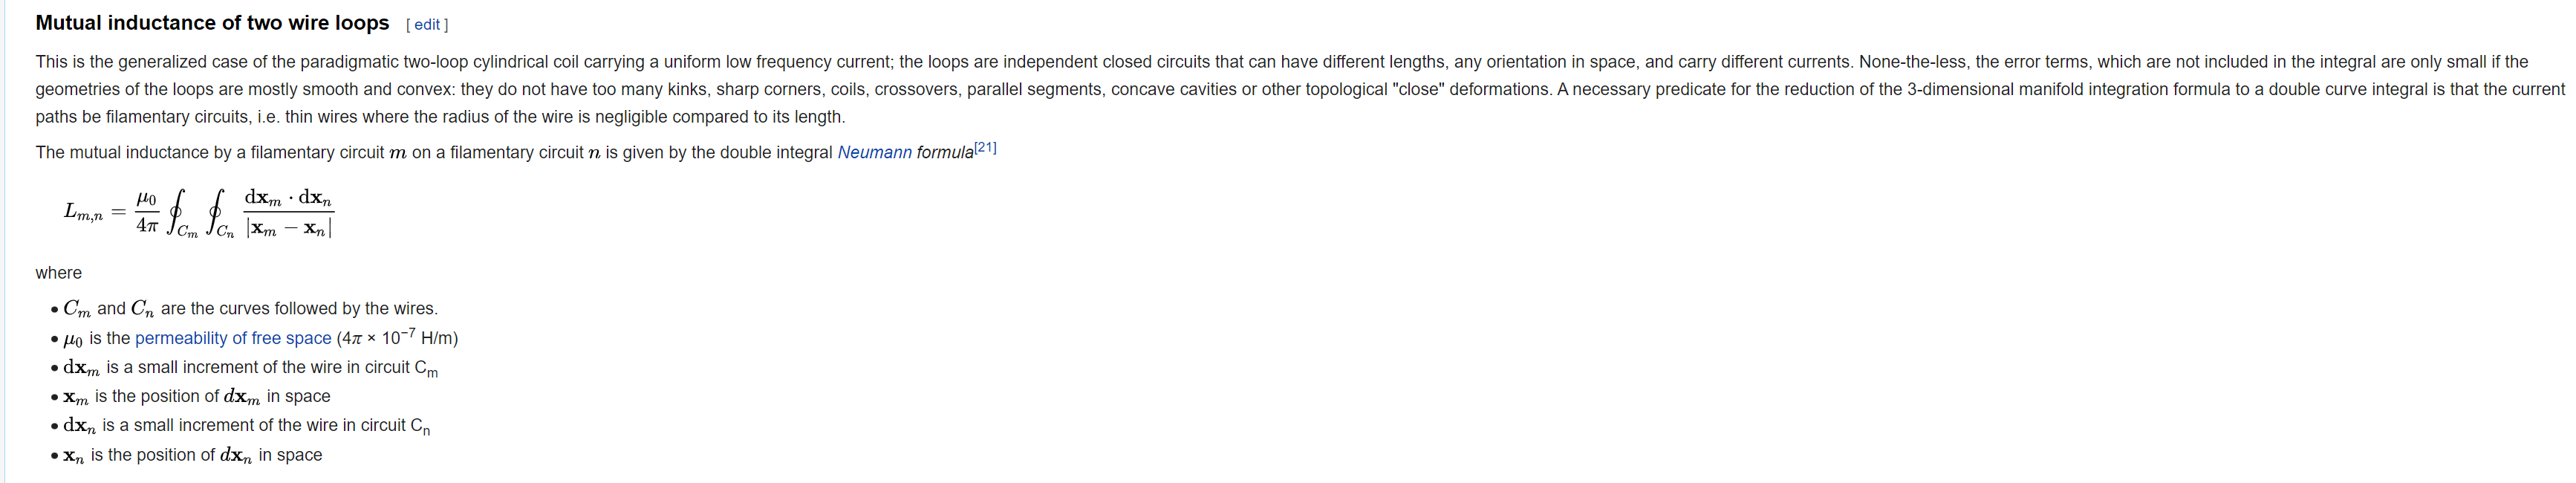
\includegraphics[width=\textwidth]{figures/mutual_inductance.png}
    \caption{\textcolor{red}{Here is an integral that computes mutual inductance. I think it would be worth comparing this to the Gauss linking integral which can also be computed via Alexander duality. That and the intersection product. Using alexander duality there are probably some more interesting products that can be computed. Examples with coils would be good since the magnetic field they generate will link the coils and drive current in the disconnected circuit components.}}
\end{figure}

\subsection{Circuits}
Need some notion of what the heck a circuit is. 
I guess we can define it as a collection of conductors? 
A conductor being a spatial 3-manifold we remove from $S^3$?

Series and parallel may be helpful to think about. 
Are things that are "in series" defined on the conductor and the "in parallel" as being defined on the complement? 
Alexander duality stuff?

\subsection{Ammeter}
Connected in series with the circuit. 
Low resistance so all current flows through this. 
It is only a first absolute (maybe relative???) homology class of the complement to the circuit? Dual to relative classes inside the conductor via Alexander and POincare duality. 
In essence, you split the conductor into two connected components and reglue them together with the ammeter.

Okay, but how does a real ammeter actually work? 
\begin{figure}
    \centering
    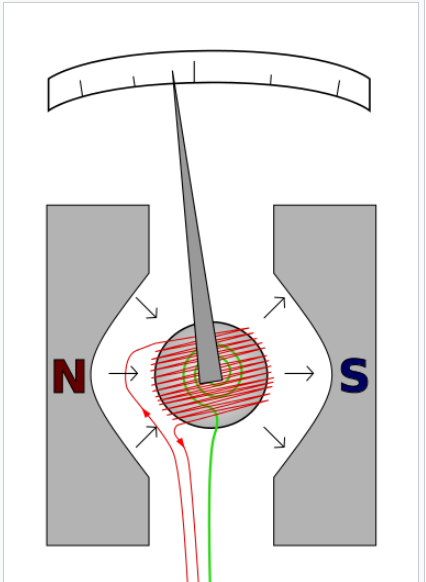
\includegraphics{figures/ammeter.png}
    \caption{Ammeter}
\end{figure}
Red wires are connected to the circuit and induce a force on the needle to overcome the spring. 
How much the needle is deflected is proportional to the current.
So actually you never measure current directly I guess. 
YOu just measure what magnetic fields do. 
I don't know if this is a philosophical distinction or what.

\subsection{Voltmeter}
Connected in parallel with the circuit. 
High resistance so it doesn't steal current from the circuit. 
So ours should probably be infinite resistance so no current flows along it.
In other words, it has no first absolute homology in the complete to the circuit?

If I'm not mistaken, a voltmeter uses an ammeter but places a Ohmic resistor in the red wire so that the current is proportional now to voltage difference. 
But maybe a better way to think about it is that it is a map of the zero sphere into the conductor where you then subtract the values at each point the zero sphere lands. 
That would also be like a "wire" with infinite resistance.
In that case, it is like you look at the image of the boundary map of a relative 1 cycle chain on the complement to the conductor and by integration and stokes theorem, you'd get the difference of the potential on the boundary of the relative 1 cycle.

\subsection{Ohmmeter}
Applies a current to the circuit and measures the resulting voltage. 
So it is a product of a voltmeter and current in some way.


\begin{figure}
    \centering
    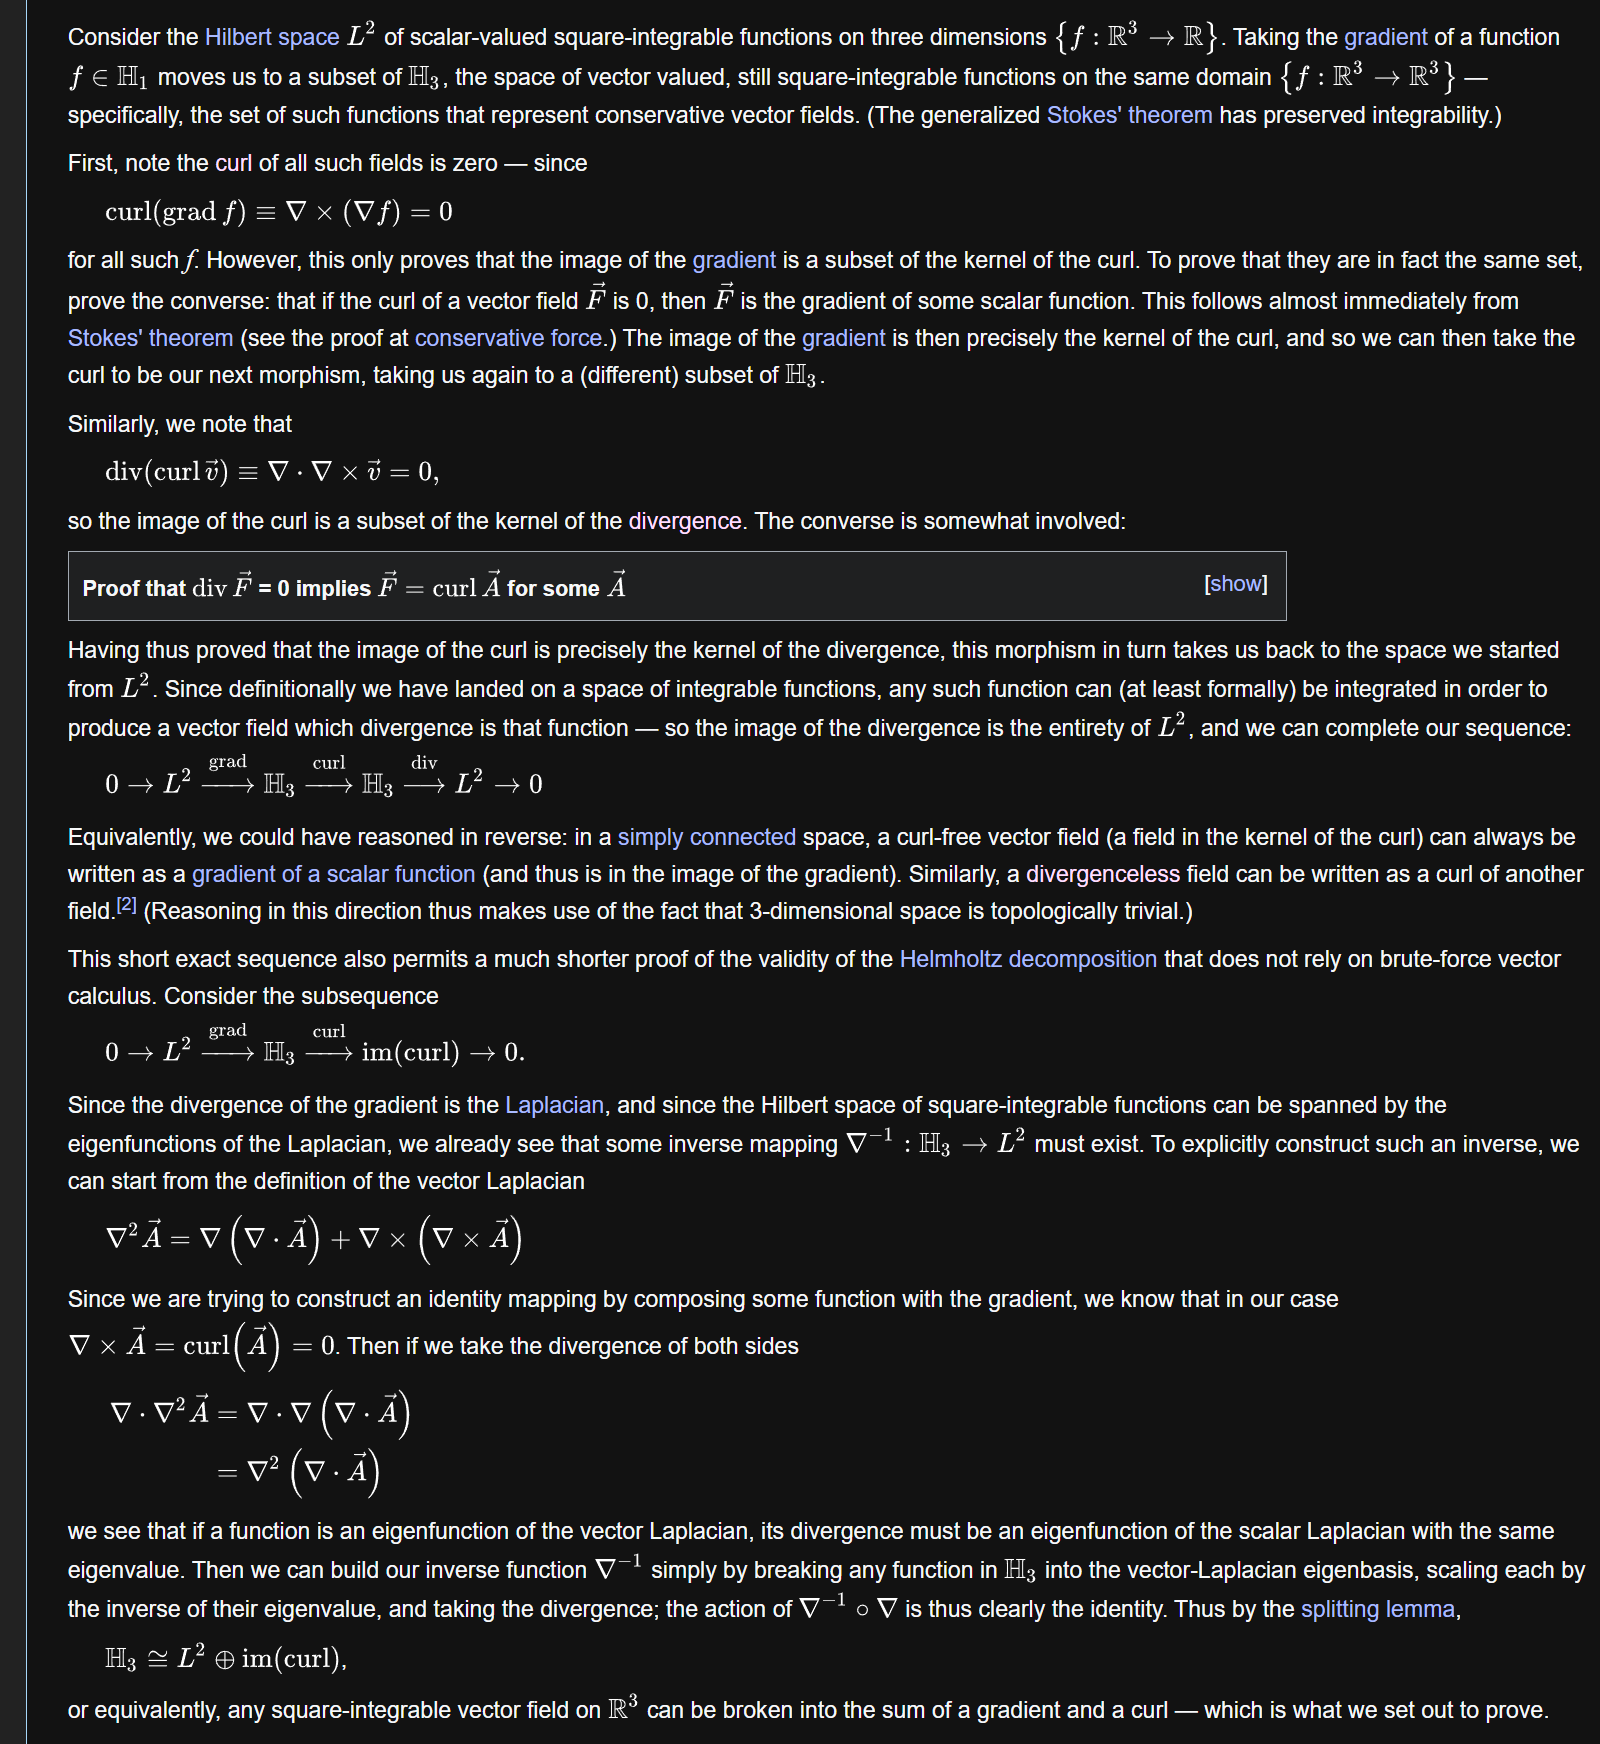
\includegraphics[width=\textwidth]{figures/splitting.png}
    \caption{I like this explanation on the Exact Sequence wikipedia page}
\end{figure}


\bibliographystyle{unsrt}
\bibliography{main}

\end{document}
%---------------------------------------------------------------------------------------------------------------------------